% -*- CODING:iso-8859-1; TeX-PDF-mode:t -*-

\RequirePackage[ngerman=ngerman-x-latest]{hyphsubst}
\documentclass[fontsize=11pt,listof=totoc,index=totoc]{scrartcl}
\usepackage[latin1]{inputenc}
\usepackage[T1]{fontenc}
\usepackage{%
  graphicx,
  longtable,
  fixltx2e,
  mparhack,
  url,
  xcolor,
  ragged2e,
  setspace,
  pifont,
  bera,
  fancyvrb,
}

\usepackage[english,ngerman]{babel}
\usepackage[neveradjust]{paralist}
%\usepackage[babel,german=guillemets-italics]{csquotes} 
\usepackage[babel,german=guillemets]{csquotes}
\MakeAutoQuote{�}{�}
\usepackage{microtype}

\usepackage{makeidx}
\makeindex

\definecolor{uibkorange}{HTML}{F89019} % Studium
\definecolor{uibkgruen}{HTML}{74A629} % Forschung
\definecolor{uibkblau}{HTML}{002241} % Uibkversit�t
\definecolor{uibkcyan}{HTML}{419AB9} % Fakult�ten
\definecolor{uibkviolett}{HTML}{5E4683} % Internationales
\definecolor{uibkrot}{HTML}{CB0900} % iPoint


\usepackage{float}
\usepackage{marginnote}
\renewcommand*{\marginfont}{\color{uibkrot}\sffamily\bfseries}

\newenvironment{Hinweis}
{\bigskip\reversemarginpar\marginnote[\raggedleft{Hinweis:}]{}\begin{em}\noindent\ignorespaces}
{\end{em}\hspace{\stretch{1}}\bigskip}
 
\newcommand{\ximsterm}[1]{\emph{#1}\index{#1@\emph{#1}}}
\newcommand{\ximstermdef}[1]{\emph{#1}\index{#1@\emph{#1}|textbf}}
\newcommand{\otherterm}[1]{#1\index{#1}}
\newcommand{\othertermdef}[1]{#1\index{#1|textbf}}

\addtokomafont{sectioning}{\color{uibkcyan}}
\addtokomafont{sectionentrypagenumber}{\color{black}}
\addtokomafont{caption}{\small}
\addtokomafont{captionlabel}{\small}

\setlength{\skip\footins}{1.05\baselineskip}
\setkomafont{footnotelabel}{\bfseries}
\deffootnote[0em]{0pt}{1.0em}{\thefootnotemark~}
\makeatletter
\renewcommand*\footnoterule{%
  \kern-4.9\p@% Platz unter der Linie + Liniendicke
  \ifx\@textbottom\relax\else\vskip \z@ \@plus.05fil\fi
  \hrule\@width.4\columnwidth
  \kern 4.5\p@}% Platz unter der Linie
\makeatother

\usepackage[%
breaklinks               % Links ��berstehen� Zeilenumbruch
,backref                 % Backlinks im Literaturverzeichnis
,colorlinks              % Links erhalten Farben statt K�sten
,citecolor=black      % Farbe f�r Zitate
,linkcolor=black     % beeinflusst Inhaltsverzeichnis und Seitenzahlen
,urlcolor=black         % Farbe f�r URLs
,citecolor=black       % Farbe f�r Zitate
,linkcolor=black       % beeinflusst Inhaltsverzeichnis und Seitenzahlen
,urlcolor=black 
,bookmarks               % Erzeugung von Bookmarks f�r PDF-Viewer
,bookmarksnumbered       % Nummerierung der Bookmarks
,hyperfootnotes=false    % Keine Links auf Fu�noten
%,hyperindex=false        % Vorerst keine Hyperlinks im Index, 
                         % siehe http://wwwmath.uni-muenster.de/u/mollerh/data/Hyper.pdf
,pdffitwindow
,pdflang=de
,pdfpagelabels 
%,pdfborder={0 0 0}
,pdfpagelayout=SinglePage
,pdftitle={XIMS Schritt f�r Schritt Anleitung}
,pdfauthor={xims-support@uibk.ac.at}
,pdfsubject={}
,pdfkeywords={}
,pdfcreator={pdfTeX}
,pdfstartview=FitV,      % Dokument wird �Fit Height� ge�ffnet
,pdfpagemode=UseOutlines % Bookmarks im Viewer anzeigen
,bookmarksopenlevel=2    % Gliederungstiefe der Bookmarks
] 
{hyperref}               % PDF automatisch mit Links versehen und weitere
% Hypertext-Funktionalit�t erm�glichen

\usepackage{ellipsis}

\title{XIMS Schritt f�r Schritt Anleitung}
\author{\href{mailto:XIMS-Support@uibk.ac.at}{\nolinkurl{XIMS-Support@uibk.ac.at}}}
\date{\today}

\widowpenalty=300
\clubpenalty=300

\hyphenation{De-part-ment-Root}
\hyphenation{De-part-ment-Links}
\hyphenation{Sup-port}

\begin{document}

\maketitle
\setcounter{tocdepth}{3}

\tableofcontents
\newpage


%\tableofcontents
%\newpage

\section{Allgemeines zum System}
\label{allgemeines}

\othertermdef{XIMS} (eXtensible Information Management System) ist ein
Web-Content-Management- und Informationssystem, das vor allem auf die
Anforderungen und Bed�rfnisse von Universit�ten und �hnlichen
Institutionen zugeschnitten ist.

Daraus ergeben sich unter anderem folgende Entwicklungsziele, die
\otherterm{XIMS} zu erf�llen versucht:
\begin{compactitem}
\item Einfache Einbringungsm�glichkeiten, um die Verwaltung der
  Inhalte m�glichst unabh�ngig von technischem Know-how zu
  erm�glichen.
\item Granulares Berechtigungssystem bzw. Rollenmanagement, um die
  Aufgaben und Verantwortungsbereiche verschiedener Benutzer zu
  verwalten.
\item Flexible Gestaltungsm�glichkeit der zu pr�sentierenden Inhalte
  durch Trennung von Formatierung und Inhalt (realisiert durch die
  Verwendung von XML in Zusammenhang mit \otherterm{XSLT}).
\item Delegierbarkeit von Berechtigungen f�r dezentrale Verwaltung von
  Inhalten und Benutzern.
\item Unterst�tzung mehrsprachiger Inhalte.
\end{compactitem}

Neben den genannten Entwicklungszielen bietet die folgende Liste eine Auswahl von
n�tzlichen \otherterm{XIMS} Features:
\begin{compactitem}
\item Klare Strukturierung von Inhalten durch sprechende, leicht
  merkbare Adressen (Stichwort \ximsterm{Kurznamen}).
\item �bersichtliche Navigation durch den Inhalt (Verwendung eines
  �Breadcrumb- Navigations-Pfades�).
%\item Flexible Suchm�glichkeiten unterst�tzt durch Google.
\item M�glichkeit der Generierung von Dublin Core Metadaten f�r
  \otherterm{XIMS} Inhalte und Objekte.
\end{compactitem}    

\otherterm{XIMS} wurde am Zentralen Informatikdienst der Universit�t
Innsbruck entwickelt und ist als freie Software ver�ffentlicht worden
(\url{http://xims.info/download}). F�r allgemeine Fragen und Fragen
zur Benutzung wenden Sie sich bitte an den \otherterm{XIMS}-Support,
f�r technische Fragen, Bug-Meldungen oder gew�nschte Features bitte an
\href{mailto:xims-devel@lists.sourceforge.net}{\nolinkurl{xims-devel@lists.sourceforge.net}}.


\subsection{Anmeldung}
\label{anmeldung}

\begin{figure}[H]
  \centering
  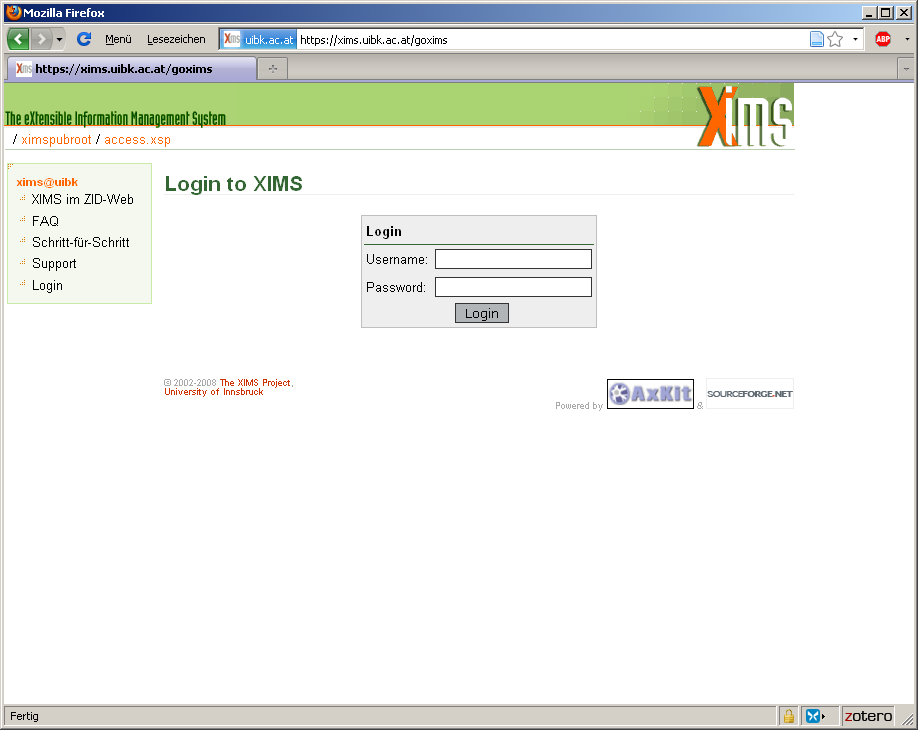
\includegraphics[width=1.00\textwidth]{./images/xims-login.png}
  \caption{\otherterm{XIMS} Anmeldemaske}
  \label{fig:xims-login}
\end{figure}

\otherterm{XIMS} ist an der Uni Innsbruck unter der Adresse
\url{https://xims.uibk.ac.at} zu erreichen. Um Inhalte �ber
\otherterm{XIMS} verwalten zu k�nnen, ben�tigt man einen g�ltigen
\otherterm{Benutzerzugang} (Account). UIBK"=Mitarbeiter/"=innen
erlangen mit der Akkreditierung �ber die Personalabteilung automatisch
einen Zugang zu \otherterm{XIMS}. Durch die Eingabe des Benutzernamens
(beginnt i.\,d.\,R. mit �c�) und des Passworts (normalerweise selbes
Passwort wie am Mail-System) in der \otherterm{XIMS}-Anmeldemaske
(siehe Abb.~\ref{fig:xims-login}) erlangen \otherterm{XIMS}-Benutzer
Zugang zum System.

\subsection{Schnelleinstieg -� \otherterm{XIMS} in 5 Seiten}
\label{schnelleinstieg}

Der folgende Schnelleinstieg in \otherterm{XIMS} soll Benutzer/-innen
in die Lage versetzen, einfache Ver�nderungen an Webseiten in
\otherterm{XIMS} vorzunehmen. Der Schnelleinstieg ist als gek�rzte
Darstellung der Grundfunktionen gedacht und kann die
Auseinandersetzung mit den restlichen Kapiteln der
Schritt"=f�r"=Schritt"=Anleitung nicht ersetzen.

\subsubsection{Startseite mit Lesezeichen}
\label{quick-startseite}

\begin{figure}[H]
  \centering
  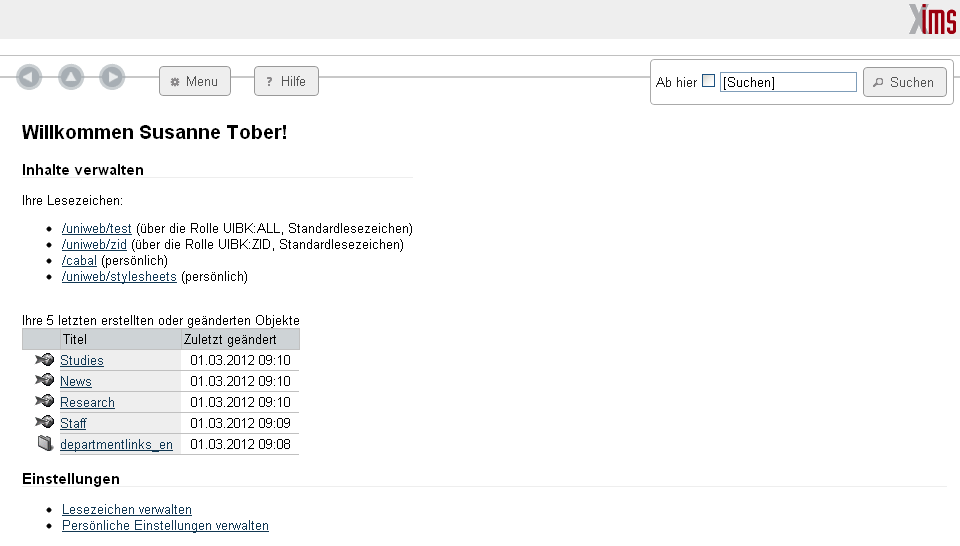
\includegraphics[width=1.00\textwidth]{./images/ximsstartseite.png}
  \caption{Benutzerspezifische \otherterm{XIMS} Startseite}
  \label{fig:ximsstartseite}
\end{figure}

Nach erfolgreicher Anmeldung wird die pers�nliche
\otherterm{XIMS}-Startseite angezeigt. Abh�ngig von den vergebenen
Rollen\footnote{Siehe Punkt \ref{rollenverwaltung}} stehen
verschiedene \otherterm{Lesezeichen} und Links auf eine Auswahl der
zuletzt erstellten oder ge�nderten Objekte zur Verf�gung.

\subsubsection{\ximsterm{Containeransicht}}
\label{quick-containeransicht}

\begin{figure}[H]
  \centering
  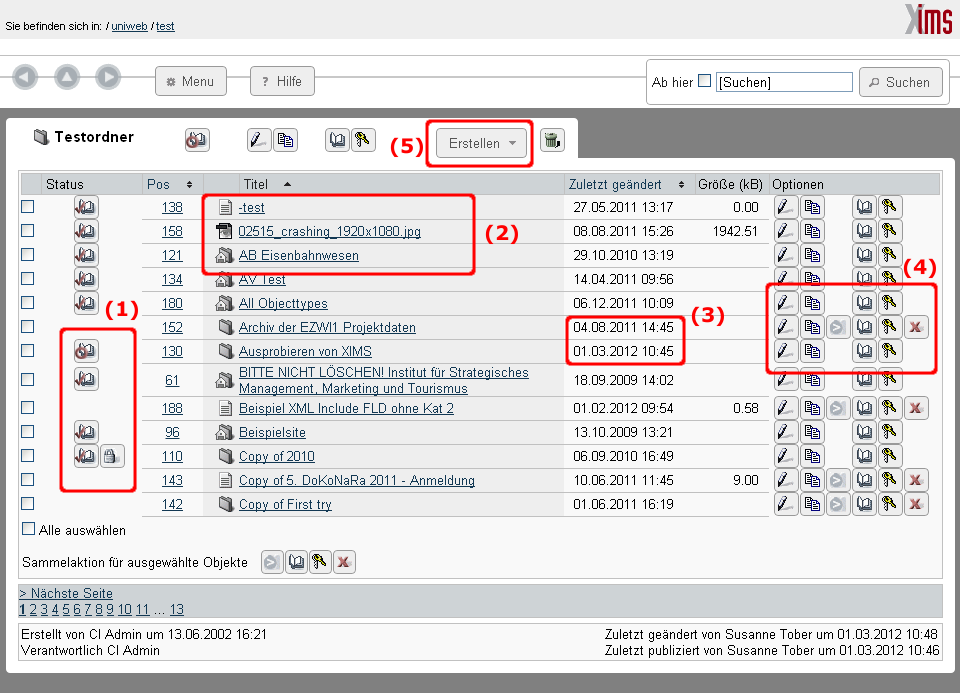
\includegraphics[width=1.00\textwidth]{./images/containeransicht1.png}
  \caption{\ximsterm{Containeransicht}}
  \label{fig:containeransicht}
\end{figure}

Die \ximstermdef{Containeransicht} gibt einen �berblick �ber die
vorhandenen Objekte und bietet verschiedene M�glichkeiten zu deren
Verwaltung an:
\begin{description}
\item[(1)] zeigt den derzeitigen \ximsterm{Objektstatus} an
  (publiziert, nicht publiziert, \dots)
\item[(2)] zeigt ein Icon f�r den \ximsterm{Objekttyp} sowie den Titel
  des Objekts
\item[(3)] zeigt das Datum der letzten �nderung
\item[(4)] zeigt m�glichen Operationen (editieren, kopieren,
  verschieben, publizieren, \dots)
\item[(5)] das Men� zum Erstellen neuer Objekte
\end{description}

\clearpage %XXX

Die unter (4) gezeigten \ximsterm{Verwaltungsoptionen} im Detail:

\begin{figure}[H]
  \centering
  
\includegraphics[width=0.4\textwidth]{./images/XI5S-optionsicons.png}
  \caption{Verwaltungsoptionen f�r Objekte}
  \label{fig:optionsicons}
\end{figure}

\begin{description}
\item[(A) \otherterm{Editieren}] �ffnet eine Bearbeitungsansicht
  (z.\,B. den Editor bei Dokumenten)
\item[(B) \otherterm{Kopieren}] Stellt vom gew�hlten Objekt eine Kopie
  her (Bsp: Copy~of~Test)
\item[(C) \otherterm{Verschieben}\footnote{Steht nur zur Verf�gung
    wenn das Objekt \emph{nicht} publiziert ist.}] �ffnet ein Men� zum
  Verschieben des Objekts
\item[(D) \otherterm{Publizieren}] �ffnet das Men� zum Ver�ffentlichen
  von Objekten
\item[(E) \otherterm{Rechte verwalten}] �ffnet die Rechteverwaltung
\item[(F) \otherterm{L�schen}\footnote{Steht nur zur Verf�gung wenn
    das Objekt \emph{nicht} publiziert ist.}] L�scht das Objekt (siehe
  Punkt \ref{delete}: Objekte l�schen und �Papierkorb�)
\end{description}

\subsubsection{Erstellen von Objekten}
\label{quick-erstellen}

Mit Hilfe des Erstellen-Men�s (5) k�nnen verschiedene
\ximstermdef{Objekttyp}en\footnote{Abh�ngig von den Benutzerrechten}
erstellt werden. Die Standardobjekttypen lauten:

Dokument (\ximsterm{Document}), Datei (\ximsterm{File}), Ordner
(\ximsterm{Folder}), Bild (\ximsterm{Image}), \ximsterm{Text} und
\ximsterm{URLLink}\footnote{Siehe Punkt \ref{urllinks}}.
\ximsterm{File} kann prinzipiell jede\footnote{Zumeist wird es sich um
  bin�re Dateitypen handeln. In Ausnahmef�llen kann es aber auch
  sinnvoll sein zu tricksen und z.\,B. HTML-Dateien als
  \ximsterm{File} mit der Endung \path{.htm} am System vorbeizumogeln}
Datei sein (z.\,B. eine PDF-Datei, eine MS-Word-Datei, ...) -- einzig
Bilder sollten stets �ber den Men�punkt Bild (Image) erstellt werden,
denn nur so ist sichergestellt, dass die Bilder sp�ter problemlos in
den verschiedenen Bild-Einf�gen-Dialogen aufgefunden werden k�nnen.

\begin{figure}[!ht] 
  \centering
  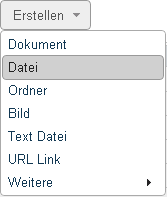
\includegraphics[width=0.25\textwidth]{./images/create-menu.png}
  \caption{Erstellen-Men�}
  \label{fig:erstellenmenu}
\end{figure}

Ein Klick auf den jeweiligen Men�punkt �ffnet den Dialog zum Erstellen
des Objekts. Dieser �hnelt dem Dialog zum Bearbeiten eines Dokuments
und wird im folgenden Abschnitt beschrieben.

\subsubsection{Editieren von Objekten}
\label{quick-editieren}

Jedes Objekt in Xims (mit wenigen Ausnahmen) hat einen \ximsterm{Titel} und 
%eine \ximsterm{Location}.
einen \ximsterm{Pfad}.

Der \ximsterm{Titel}, in unserem Beispiel �Schritt f�r Schritt�, wird
sp�ter in der Containeransicht aufscheinen. Beim \ximsterm{Objekttyp}
\ximsterm{Document} wird aus diesem Feld das HTML-Element
\texttt{<title>} erzeugt, der Titel erscheint im publizierten Dokument
in der Titelleiste des Browserfensters.

%Die \ximsterm{Location} 
Der Pfad 
ist der Dateiname eines Objekts. Wird das Dokument
ver�ffentlicht,\footnote{Siehe dazu Punkt \ref{quick-publizieren}.} so
findet man den Eintrag 
des Pfades
%der \ximsterm{Location} 
in der \otherterm{URL}
wieder. Deshalb sind in diesem Feld nur Kleinbuchstaben und keine
Umlaute, Sonder- oder Leerzeichen erlaubt. Die Dateiendung
(\path{.doc}, \path{.pdf}, \path{.html}, etc.) wird vom System beim
Speichern abh�ngig vom \ximsterm{Objekttyp} und Datenformat
automatisch hinzugef�gt.

Sobald Sie die Eingabe eines Titels abgeschlossen haben, wird automatisch 
%eine \ximsterm{Location} +
ein Pfad 
generiert, die diesen Vorgaben entspricht. Aus dem Titel �Schritt f�r Schritt� wird 
%die Location 
der Pfad 
�schritt-fuer-schritt.html�. 
%Diese Location 
Dieser Pfad 
ist als ein Vorschlag vom System zu sehen und kann von Ihnen noch ge�ndert werden. 

%Deshalb sollte zum einen eine m�glichst selbsterkl�rende und leicht zu merkende Bezeichnung der \ximsterm{Location} vergeben werden, zum anderen bestehen deshalb gewisse Beschr�nkungen f�r den Feldinhalt. So sind im Feld \ximsterm{Location} nur Kleinbuchstaben und keine Umlaute, Sonder- oder Leerzeichen erlaubt. Die Dateiendung (\path{.doc}, \path{.pdf}, \path{.html}, etc.) wird vom System beim Speichern abh�ngig vom \ximsterm{Objekttyp} und Datenformat automatisch hinzugef�gt.


\begin{figure}[!ht]
  \centering
  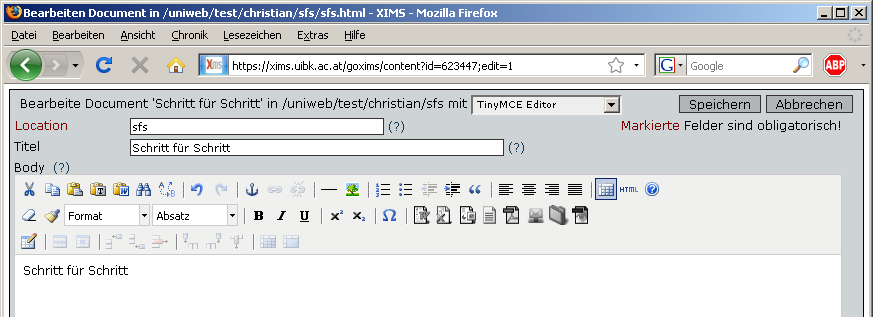
\includegraphics[width=1.00\textwidth]{./images/XI5S-dokument-tinymce.png}
  \caption{Dokument im TinyMCE Editor}
  \label{fig:XI5S-dokument-tinymce}
\end{figure}

Die Benutzeroberfl�che des \otherterm{TinyMCE}-Editor �hnelt jener von
MS-Word, Die verschiedenen Bedienelemente sind gr��tenteils analog
verwendbar. Ist der Editiervorgang abgeschlossen, so k�nnen die
�nderungen mit einem Klick auf den �Speichern�-Button gespeichert
oder mit �Abbrechen� verworfen werden.

\begin{Hinweis}
  Navigieren Sie nicht mit der �Vor�- und �Zur�ck�-Taste ihres
  Browsers aus dem Editor, weil das bearbeitete Objekt ansonsten f�r
  andere Benutzer gesperrt wird.\footnote{Siehe Punkt \ref{gesperrteobjekte}
  �Gesperrte Objekte�.}
\end{Hinweis}



\subsubsection{Ver�ffentlichen von Objekten}
\label{quick-publizieren}

Ein in \otherterm{XIMS} erstelltes Objekt ist der �ffentlichkeit nicht
sofort zug�nglich. Es befindet sich zuerst lediglich in
\otherterm{XIMS} selbst. Um es �ber den �ffentlichen Webserver
abrufbar zu machen, muss es zuerst in einem eigenen Schritt
ver�ffentlicht werden. Beim erstmaligen \otherterm{Publizieren} eines
neu erstellten Objekts erscheint folgendes \otherterm{Dialogfenster}
(siehe Abb.~\ref{fig:XI5S-publish}), das �Ver�ffentlichen� oder
�Abbrechen� zur Auswahl stellt.

\begin{figure}[ht!]
  \centering
  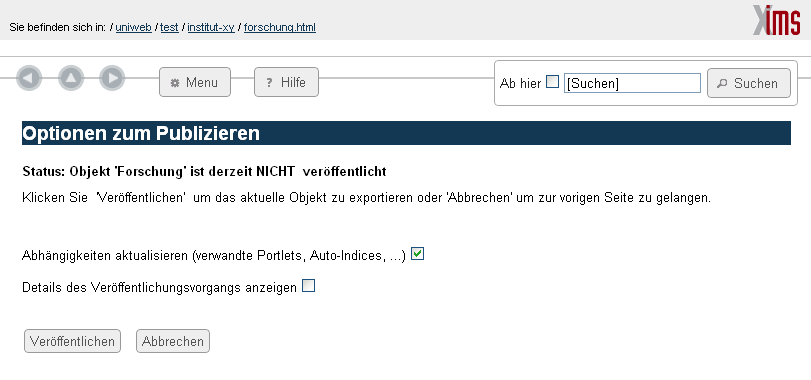
\includegraphics[width=\textwidth]{./images/XI5S-publish.png}
  \caption{Ver�ffentlichen eines Objekts}
  \label{fig:XI5S-publish}
\end{figure}

Wurden an einem ver�ffentlichten Objekt �nderungen vorgenommen, so
muss das Objekt �wiederver�ffentlicht� werden, um die aktualisierte
Version auf den Webserver zu schreiben. Die Operation �Ver�ffentlichen
r�ckg�ngig machen� nimmt ein Objekt wieder aus dem �ffentlichen
Bereich.\footnote{Nachdem die Ver�ffentlichung r�ckg�ngig gemacht
  wurde, stehen Optionen wie beispielsweise �verschieben� oder
  �l�schen� wieder zur Verf�gung.}.

\begin{figure}[H]
  \centering
  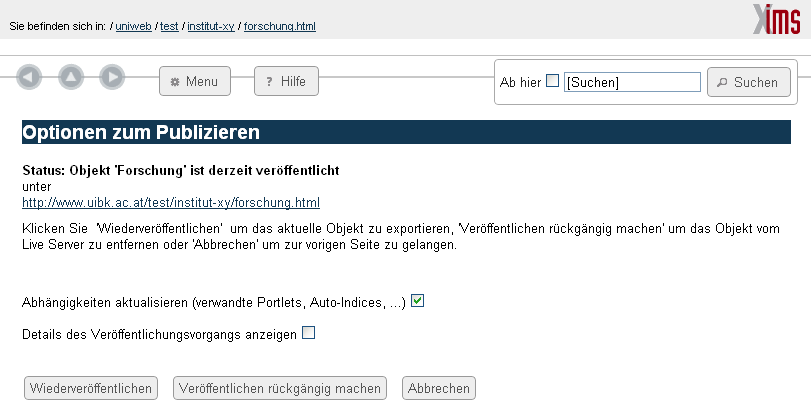
\includegraphics[width=\textwidth]{./images/XI5S-republish.png}
  \caption{Dialog Wiederver�ffentlichen/Ver�ffentlichen r�ckg�ngig machen}
  \label{fig:XI5S-republish}
\end{figure}


\clearpage
\section{Startseite und allgemeiner Aufbau}
\label{startseite}

Nach erfolgreicher Anmeldung gelangt man zur pers�nlichen Startseite
im \otherterm{XIMS} Content-Management-System.

\begin{figure}[!ht]
  \centering
  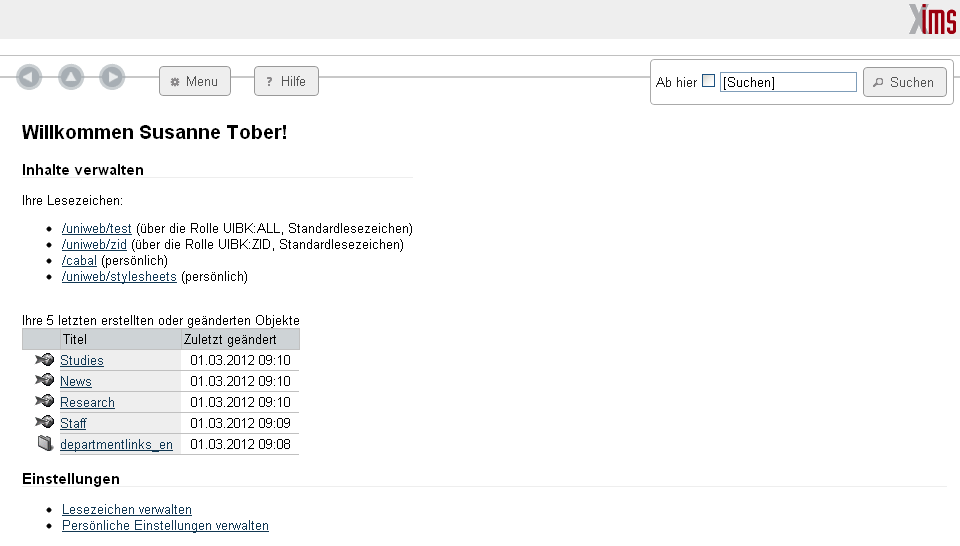
\includegraphics[width=0.90\textwidth]{./images/ximsstartseite.png}
  \caption{Benutzerspezifische \otherterm{XIMS} Startseite}
  \label{fig:ximsstartseite2}
\end{figure}

F�r alle Benutzer/-innen sind \otherterm{Lesezeichen} (Bookmarks)
konfiguriert.\footnote{Universit�ts-Mitarbeiter/-innen bekommen
  automatisch in eine Mitarbeiter/-innen-Rolle zugewiesen; �ber diese
  sind sie berechtigt, im {XIMS}-Testordner Objekte zu erstellen und
  erhalten ein entsprechendes Lesezeichen.} Diese Lesezeichen h�ngen
entweder von Rollen ab oder k�nnen oder k�nnen �ber �Lesezeichen
verwalten� gesetzt, gel�scht und ver�ndert werden. Dort kann auch das
\othertermdef{Standardlesezeichen} (default Bookmark) gew�hlt werden.
Das \otherterm{Standardlesezeichen} bewirkt eine automatische
Weiterleitung von der Einstiegsadresse
\url{https://xims.uibk.ac.at/goxims/defaultbookmark} aus auf das
gew�hlte Ziel.



\begin{Hinweis}
  Nutzen Sie den \otherterm{XIMS}-Testordner um sich mit dem System
  vertraut zu machen. Dort k�nnen Sie Objekte erstellen und das
  allgemeine Verhalten von \otherterm{XIMS} testen.
\end{Hinweis}

Typischerweise bekommen Sie �ber die Rolle Ihrer Organisationseinheit
automatisch ein \othertermdef{Lesezeichen} zu deren Verzeichnis. Unter �Lesezeichen
verwalten� k�nnen Sie beliebige weitere Lesezeichen erstellen, um
schnell und bequem auf oft ben�tigte Objekte zugreifen zu k�nnen.

Verzeichnisse erscheinen in der \ximsterm{Containeransicht}:

\begin{figure}[!ht]
  \centering
  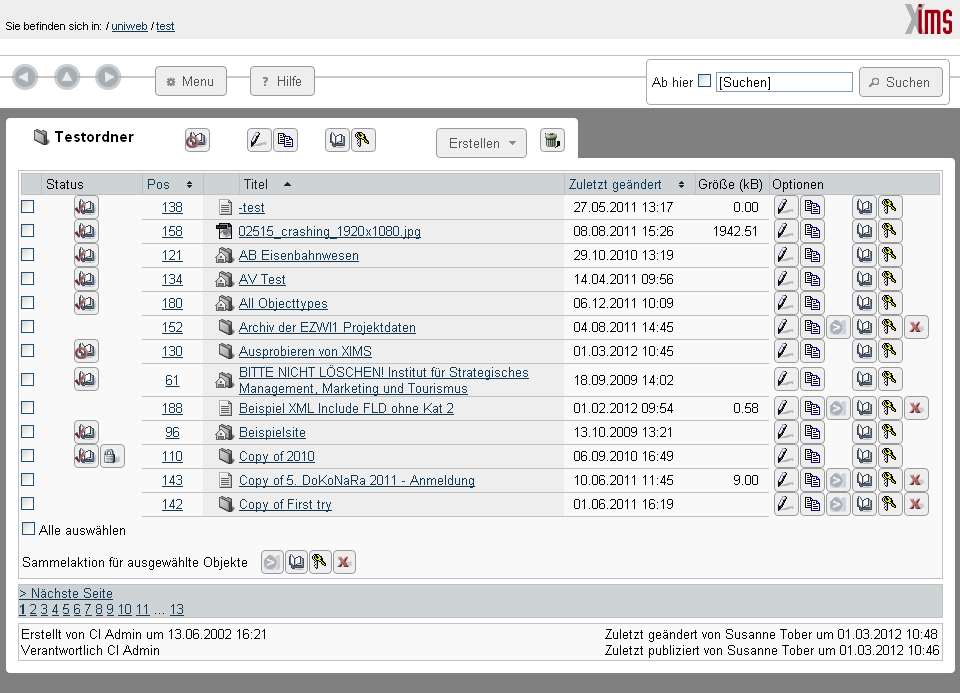
\includegraphics[width=0.90\textwidth]{./images/containeransicht.png}
  \caption{\otherterm{XIMS} \ximsterm{Containeransicht}}
  \label{fig:containeransicht2}
\end{figure}

\subsection{Navigation}
\label{navigation}

Der \otherterm{XIMS}-\ximsterm{Navigationsbereich} besteht unter anderem aus den folgenden Elementen:

\paragraph{Aktueller Pfad (Navigations-/Breadcrumb-Pfad)}
\label{breadcrumb}

\begin{figure}[!ht]
  \centering
  
\includegraphics[scale=0.7]{./images/navigationspfad.png}
  \caption{Navigations-/Breadcrumb-Pfad}
  \label{fig:navigationspfad}
\end{figure}


Der \ximstermdef{Navigationspfad} zeigt den Pfad vom
�\ximstermdef{SiteRoot}� (f�r \url{http://www.uibk.ac.at/} hei�t das
\ximsterm{SiteRoot} \path{uniweb}) bis zum aktuellen Objekt an. Das
Anklicken eines Teilpfades erm�glicht ein schnelles Wechseln in einen
�bergeordneten \ximsterm{Container}. Die Pfadfragmente (z.\,B.
\path{uniweb}) entsprechen dabei dem �\ximsterm{Location}�-Attribut
des \ximsterm{Container}s.

\paragraph{Navigationspfeile}
\label{navigationspfeile}

\begin{figure}[!ht]
  \centering
  
\includegraphics[scale=0.7]{./images/navigationspfeile.png}
  \caption{Navigationspfeile}
  \label{fig:navigationspfeile}
\end{figure}

Die \ximstermdef{Navigationspfeil}e erm�glichen ein schnelles Bewegen
innerhalb des Systems: einen Schritt zur�ck (back), eine Ebene h�her
im Verzeichnisbaum (one level up), oder einen Schritt vorw�rts
(forward).

\paragraph{Login-Informationen}
\label{logininfo}

\begin{figure}[!ht]
  \centering
  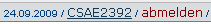
\includegraphics[scale=0.7]{./images/logininfo.png}
  \caption{Login-Informationen}
  \label{fig:logininfo}
\end{figure}

Die Login-Informationen beinhalten das aktuelle Datum, den Namen des
angemeldeten Benutzers und die M�glichkeit sich �ber �logout� vom
System abzumelden.

\paragraph{Element zum Erstellen von neuen Objekten}
\label{newobject}

\begin{figure}[!ht]
  \centering
  
\includegraphics[scale=0.7]{./images/button-create.png}
  \caption{Element zum Erstellen von neuen Objekten}
  \label{fig:erstellenbutton}
\end{figure}

Diese Option wird unter Punkt \ref{erstelleneditieren} ausf�hrlich
beschrieben.\footnote{Die Option ist nur sichtbar, wenn die n�tigen
  Rechte zum Erstellen (\ximsterm{Objekttypprivilegien}) vergeben
  wurden. Falls sie fehlt, wurde Ihnen m�glicherweise versehentlich
  keine Rolle zugewiesen; wenden Sie sich bitte an
  \href{mailto:XIMS-Support@uibk.ac.at}{\nolinkurl{XIMS-Support@uibk.ac.at}}}

\paragraph{\otherterm{Suchfunktion}}
\label{suche}

\begin{figure}[!ht]
  \centering
  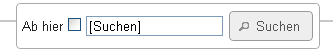
\includegraphics[scale=0.7]{./images/suche.png}
  \caption{Suchfunktion}
  \label{fig:suchfunktion}
\end{figure}

Ein Suchausdruck kann aus einem oder mehreren W�rtern bestehen und bis
zu 55 Zeichen lang sein. Begriffe k�nnen auch wie �blich mit Klammern
und Operatoren zu komplexeren Ausdr�cken zusammengef�gt werden:

\begin{itemize}
\item AND
\item OR
\item ()
\end{itemize}

\begin{Hinweis}
  Um beispielsweise nach einem Objekt, welches die Begriffe �zid�
  sowie einen der Begriffe �antrag� oder �dokument� beinhaltet zu
  finden, k�nnen Sie folgenden Suchausdruck verwenden: \texttt{zid AND
    (antrag OR dokument)}
\end{Hinweis}

Folgende Ausdr�cke d�rfen nur alleine stehen:

\begin{description}
\item[M:<Tage>] Finde Objekte, die in den letzen <Tagen> ver�ndert
  wurden. <Tage> muss nicht unbedingt angeben werden, der Vorgabewert
  ist 1.
\item[N:<Tage>] Finde Objekte, die in den letzen <Tagen> erstellt
  wurden. <Tage> muss nicht unbedingt angeben werden, der Vorgabewert
  ist 1.
\item[m:<Tage>, n:<Tage>] Wie oben, aber schr�nke die Suche zus�tzlich
  auf Objekte ein, die als neu markiert wurden.
\end{description}

Die Option �Ab hier� schr�nkt die Suche auf Objekte ein, die sich in
der Verzeichnishierarchie unterhalb des aktuellen Objektes befinden.

\subsection{Ansicht von Containerinhalten}
\label{containeransicht}

Die Ansicht �ber den Containerinhalt bietet einen �berblick der im
jeweiligen \ximstermdef{Container} enthaltenen Objekte. Die Objekte
(Dateien, Ordner, HTML-Seiten, etc.) werden tabellarisch aufgelistet
und k�nnen nach verschiedenen Kriterien auf und absteigend sortiert
werden, indem auf die �berschrift der jeweiligen Spalte (�Pos�,
�Title� oder �Last Modified�) geklickt wird. (Standarddarstellung ist
aufsteigend nach der Positionsnummer).

Die Tabelle mit den Objekten setzt sich aus folgenden Spalten zusammen:

\begin{itemize}
\item Status
\item Position (Pos)
\item Titel (Title)
\item Zuletzt ge�ndert (Last Modified)
\item Gr��e des Objekts (Size)
\item Optionen zum Verwalten der Objekte (Options)
\end{itemize}

Jedem Objekt entspricht eine Zeile in der Tabelle, sind viele Objekte
in Container vorhanden, wird die Ansicht paginiert und eine
entsprechende Navigation erscheint im Seitenfu�.

\subsection{Icons in \otherterm{XIMS}}
\label{icons}

\paragraph{Status}

Der \ximstermdef{Objektstatus} gibt Auskunft �ber den derzeitigen
Zustand des Objekts. In der aktuellen Version kennt \otherterm{XIMS}
vier verschiedene \ximsterm{Objektstatus}.

\begin{table}[!ht]
%\begin{minipage}{\textwidth}
\centering

\begin{tabular}{|c|p{30em}|}
  \hline
  
\includegraphics[scale=0.7]{./images/icon-new.png} & 
  \label{new}Das Objekt ist als neu markiert. \\
  \hline
  
\includegraphics[scale=0.7]{./images/icon-published.png} & 
  Das Objekt ist ver�ffentlicht. Durch Klicken auf das Symbol gelangt man
  zur ver�ffentlichten Ansicht des Objekts. \\
  \hline
  
\includegraphics[scale=0.7]{./images/icon-modified.png} & 
  Das Objekt ist bereits einmal ver�ffentlicht worden, jedoch seit der letzten
  Publikation wieder editiert worden. Durch Klicken auf das Symbol gelangt
  man zur aktuell ver�ffentlichten Ansicht des Objekts. \\
  \hline
  
\includegraphics[scale=0.7]{./images/icon-locked.png} & 
  Das Objekt ist gesperrt, �blicherweise, weil jemand anderer das Objekt gerade
  bearbeitet.\footnotemark \\
  \hline
\end{tabular}
%\end{minipage}
\caption{Status-Icons}
\end{table}
\footnotetext{Eigene Sperren (entstanden z.B. dadurch dass
    ein Editiervorgang nicht durch Speichern oder Abbrechen
    beendet wurde) k�nnen durch Klicken auf das Schloss, �fremde�
    Sperren \emph{nur} dur das Kommando \texttt{!U:<Id> oder !U:<Pfad>} im Suchfeld, aufgehoben
    werden.  Weitere Erl�uterungen dazu siehe Punkt \ref{gesperrteobjekte}}
\paragraph{Position}

Die Spalte �Pos� (Position) stellt einen Positionierungs- bzw.
Gewichtungsmechanismus zur Verf�gung, der auf individuelle Bed�rfnisse
selbst angepasst werden kann. �ber die Spalte �Pos� k�nnen Objekte in
der Inhaltsansicht eines \ximsterm{Container}s nach vorne gereiht
werden. Die M�glichkeit spezielle Positionen zu vergeben spielt bei
den \ximsterm{DepartmentLinks} (siehe auch Punkt \ref{deplinks}) und
im Zusammenhang mit dem \ximsterm{Autoindex} (siehe auch Punkt
\ref{autoindex}) eine wichtige Rolle.

\paragraph{Titel (Title)}

Der Titel des Objekts soll eine f�r sich sprechende Bezeichnung des
Objekts sein. Das Icon vor dem Titel des Objekts l�sst auf dessen
Dateityp (PDF-Dokument, MS-Word-Dokument, etc.) schlie�en. In diesem
Zusammenhang wird auf Punkt \ref{location} verwiesen, der die
wesentlichen Unterschiede zwischen Titel und \ximsterm{Location}
aufzeigt.

\paragraph{Zuletzt ge�ndert (Last modified)}

Die Spalte �Zuletzt ge�ndert� gibt �ber das Datum und die Uhrzeit der letzten
�nderung des Objekts Auskunft.

\paragraph{Gr��e (Size)}

Diese Spalte gibt die Gr��e in Kilobyte an.\footnote{Bei Containern
  wird keine Gr��e angezeigt.}

\paragraph{Options (Optionen)}

Abh�ngig von den \otherterm{Berechtigung}en auf das jeweilige Objekt
werden verschiedene Optionen zur Verwaltung angeboten:

\begin{table}[!ht]
  \centering
  \begin{tabular}{|c|p{30em}|}
    \hline
    
\includegraphics[scale=0.7]{./images/icon-edit.png} & Option zur Bearbeitung von Objekten: Durch Anklicken des Symbols
    gelangt man in die Bearbeitungsmaske, die es erlaubt, das Objekt zu
    ver�ndern.
    Siehe dazu Punkt \ref{erstelleneditieren}: �Erstellen/Editieren�. \\
    \hline
    
\includegraphics[scale=0.7]{./images/icon-move.png} & Verschieben von Objekten: Durch Anklicken des Symbols gelangt man
    in eine weitere Maske, die mit Hilfe eines �Durchsuchen� Dialoges ein
    leichtes Verschieben des Objekts in einen anderen \ximsterm{Container}
    erm�glicht. \\
    \hline
    
\includegraphics[scale=0.7]{./images/icon-publish.png} & Optionen zum Ver�ffentlichen: Durch Anklicken des Symbols und
    Best�tigen (Confirm) des folgenden Dialogs kann ein Objekt
    ver�ffentlicht (publiziert), re-publiziert bzw. die Ver�ffentlichung
    r�ckg�ngig gemacht werden. (Siehe dazu Punkt \ref{inhaltepublizieren}). \\
    \hline
    
\includegraphics[scale=0.7]{./images/icon-acl.png} & Zugriffskontrolle/Rechteverwaltung: Durch Anklicken des Symbols
    gelangt man in eine Maske, die zum einen Auskunft �ber die
    derzeitigen Zugriffsrechte f�r das Objekt gibt und zum anderen ein
    Editieren der Zugriffsrechte erm�glicht. \\
    \hline
    
\includegraphics[scale=0.7]{./images/icon-del.png} & Objekt L�schen: Durch Anklicken des Symbols und Best�tigen
    (Confirm) des folgenden Dialogs kann ein Objekt gel�scht werden.
    (Siehe auch Punkt \ref{delete}). \\
    \hline
  \end{tabular}
  \caption{Options-Icons}
\end{table}

\clearpage

\section{Objekte manipulieren}
\label{objektemanipulieren}

Standardm��ig stehen die folgenden 14 \ximsterm{Objekttyp}en zur
Auswahl\footnote{Falls nicht, wurde Ihnen m�glicherweise versehentlich
  keine Rolle zugewiesen; wenden Sie sich bitte an
  \href{mailto:XIMS-Support@uibk.ac.at}{\nolinkurl{XIMS-Support@uibk.ac.at}}}:

\begin{itemize}
\item Dokument (Document)
\item Datei (File)
\item Ordner (Folder)
\item Bildergalerie (Gallery)
\item Bild (Image)
\item \ximsterm{Portlet}
\item \ximsterm{URL-Link}
\end{itemize}

Im Untermen� �Weitere�:

\begin{itemize}
\item CSS-Datei
\item Javascript-Datei
\item Fragebogen und TAN-Liste
\item Symbolischer Link
\item Text-Datei
\item \ximsterm{simpleDocBook} (\ximsterm{sDocBookXML})
\end{itemize}

XIMS kennt neben diesen 14 noch eine Reihe weiterer
\ximsterm{Objekttyp}en, nach Bedarf werden f�r deren Erstellung
n�tige, spezielle Berechtigungen (\ximsterm{Objekttypprivilegien})
vergeben. Einige dieser \ximsterm{Objekttyp}en werden unter dem Punkt
\ref{weitereobjekte} kurz angef�hrt.

\subsection{Erstellen/Editieren}
\label{erstelleneditieren}

�ber ein Auswahlmen� (">Erstellen"<) k�nnen Objekte unterschiedlicher Typen erstellt
werden. Die Eintr�ge im Men� werden von den beschriebenen
Berechtigungen bestimmt.\\

\begin{figure}[!ht]
  \centering
  %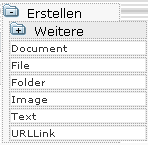
\includegraphics[scale=0.8]{./images/XI5S-erstellen-menu.png}
  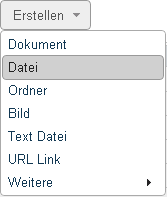
\includegraphics[scale=0.8]{./images/create-menu.png}
  \caption{Erstellen-Men�}
  \label{fig:erstellenmenu2}
\end{figure}

Um ein vorhandenes Objekt zu editieren, klickt man auf das �Bearbeiten-Icon� und
gelangt so in die Editiermaske.

\subsubsection{Dokumente}
\label{dokumente}

Ein neues Dokument kann im Webinterface auf zwei Wegen erstellt
werden: Entweder mit Hilfe von WYSIWYG-Editoren (derzeit wird von XIMS der \otherterm{TinyMCE}
Editor unterst�tzt -- siehe auch Punkt \ref{wysiwig})
oder aber mit Hilfe des �Plain Textarea� Editors. Letzterer erm�glicht
das direkte Bearbeiten des \otherterm{Quellcode}s eines Dokuments. 

Im Fenster f�r das Erstellen eines Dokuments gibt es folgende Eingabe-
bzw. Auswahlfelder:

\begin{figure}[!ht]
  \centering
  %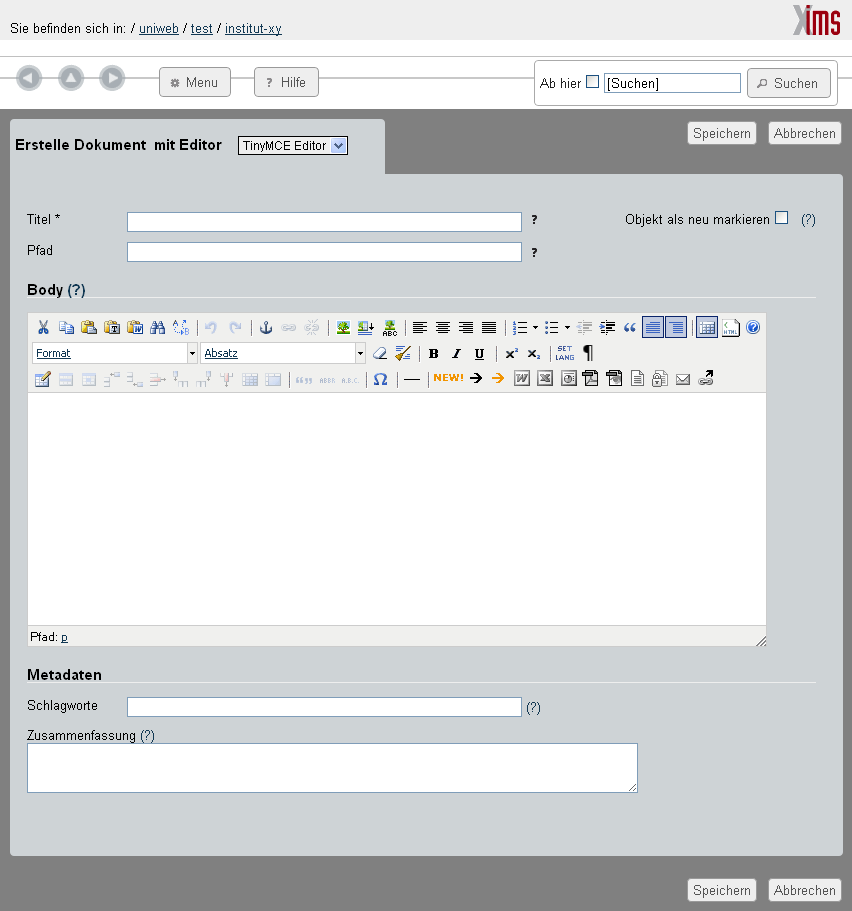
\includegraphics[width=0.9\textwidth]{./images/tinymce-full.png}
  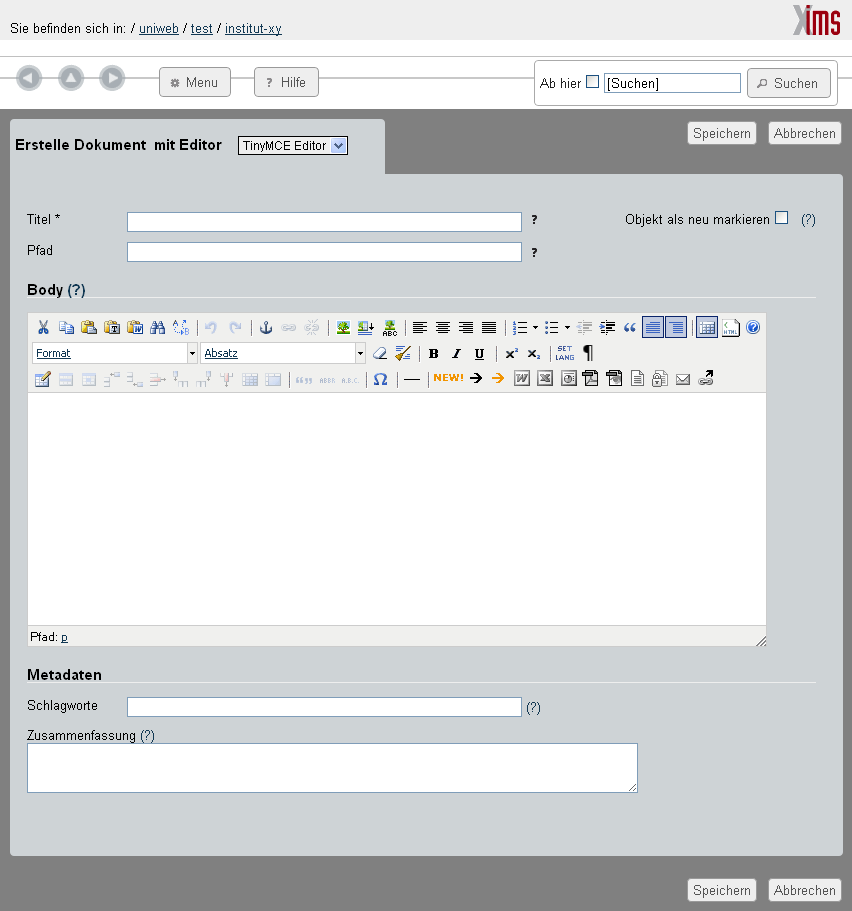
\includegraphics[width=\textwidth]{./images/tinymce-full.png}
  \caption{Erstellen eines Dokuments mit Hilfe eines WYSIWYG-Editors}
  \label{fig:dokumentwysiwyg}
\end{figure}

%\paragraph{\ximstermdef{Location}}
\paragraph{\ximstermdef{Pfad}}
\label{location}

Bei Dokumenten entspricht 
%die \ximsterm{Location} 
der Pfad dem Dateinamen des
zu erstellenden Dokuments. Wird das Dokument ver�ffentlicht (siehe
dazu Punkt \ref{publizieren}), so findet man 
den Pfad
%die \ximsterm{Location}
in der \otherterm{URL} wieder. 
Der Pfad
%Die \ximsterm{Location} 
sollte deshalb
zum einen m�glichst pr�gnant, selbsterkl�rend und leicht zu merken
sein,\footnote{Auch Suchmaschinen messen der URL als auch dem Titel
  eine besonders gro�e Bedeutung zu.} zum anderen bestehen aus dem
selben Grund auch Beschr�nkungen f�r den Feldinhalt: So sind hier
beispielsweise keine Gro�buchstaben, Umlaute, Sonder- oder Leerzeichen erlaubt. Die
Dateiendung (\path{.doc}, \path{.pdf}, \path{.html}, etc.) wird vom
System beim Speichern abh�ngig vom \ximsterm{Objekttyp} und
Datenformat automatisch hinzugef�gt. Abbildung~\ref{fig:bsppubliziert}
soll den Begriff 
%\ximsterm{Location} 
Pfad 
zus�tzlich bildlich erl�utern.


\begin{Hinweis}
  Das Feld 
  ">Pfad"<
  %�\ximsterm{Location}� 
  wird nach Eingabe eines Titels automatisch bef�llt. Dies ist ein Vorschlag des Systems und kann nach Bedarf noch angepasst werden.
\end{Hinweis}


\paragraph{Titel}
\label{title}

Der Titel, in unserem Beispiel �Schritt f�r Schritt�, entspricht dem
Namen des Dokuments, unter welchem dieses Dokument zuk�nftig in der
\ximsterm{Containeransicht} aufscheinen wird. Zudem wird der Titel
auch im \texttt{<title>} Tag des HTML-Headers ausgewiesen und
entsprechend vom Browser im Fenstertitel angezeigt. Der Titel sollte m�glichst pr�gnant und nicht zu lange gew�hlt werden.

F�r den Fall, dass kein Titel angegeben wird, wird 
%die \ximsterm{Location} 
der Pfad
auch f�r den Titel automatisch �bernommen.

\begin{figure}[!ht]
  \centering
  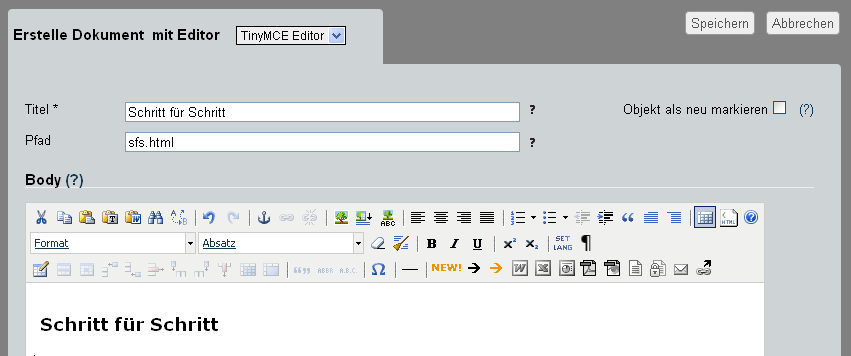
\includegraphics[width=0.9\textwidth]{./images/tinymce.png}
  %\caption{Unterscheidung: \ximsterm{Location}/Titel}
  \caption{Unterscheidung: Pfad/Titel}
  \label{fig:unterscheidunglocationtitel}
\end{figure}

In unserem Beispiel befinden wir uns im Verzeichnis
\path{/uniweb/test/institut-xy} und erstellen ein neues Dokument mit
%der \ximsterm{Location} 
dem Pfad \path{sfs.html} und dem Titel �Schritt f�r Schritt�. Das erstellte Dokument ist in \otherterm{XIMS} im
Verzeichnis \path{/uniweb/test/institut-xy} zu finden und scheint
unter dem Namen des Titels (in unserem Beispiel �Schritt f�r Schritt�)
auf.

\begin{figure}[H]
  \centering
  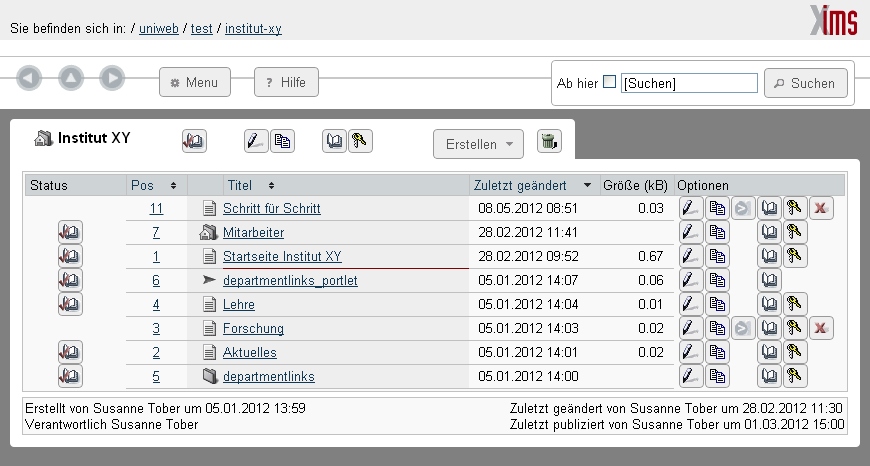
\includegraphics[width=0.9\textwidth]{./images/container-short.png}
  \caption{Ansicht des Dokuments im \otherterm{XIMS}}
  \label{fig:dokumentinxims}
\end{figure}

Abbildung~\ref{fig:bsppubliziert} zeigt das Dokument nach dem
Ver�ffentlichen auf der Universit�tswebseite.

\begin{figure}[H]
  \centering
  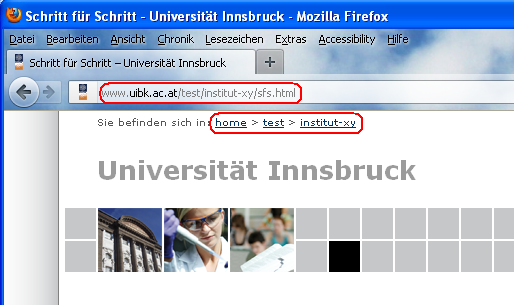
\includegraphics[width=0.9\textwidth]{./images/bsp-publiziert.png}
  \caption{Beispieldokument publiziert}
  \label{fig:bsppubliziert}
\end{figure}

Das \ximsterm{SiteRoot} \path{uniweb} und �Home� in der
Brotkr�melnavigation repr�sentieren \url{http://www.uibk.ac.at/},
darunter verlaufen die Pfade genau parallel. Hier zur Verdeutlichung
nochmals die Pfade zum Beispieldokument aus den Abbildungen:

\begin{figure}[H]
  \begin{Verbatim}[commandchars=\\\{\},fontsize=\footnotesize]
Sie befinden sich in:                                 \textbf{\textit{home}}>\textbf{test}>\textbf{institut-xy}>\textbf{sfs.html}
�ffentliche URL:                     \textbf{\textit{http://www.uibk.ac.at}}/\textbf{test}/\textbf{institut-xy}/\textbf{sfs.html}
In XIMS:     https://xims.uibk.ac.at/goxims/content/\textbf{\textit{uniweb}}/\textbf{test}/\textbf{institut-xy}/\textbf{sfs.html}
  \end{Verbatim}
  \caption{Detail: Pfade zum Beispieldokument}
\end{figure}

\paragraph{Body}
\label{body}

Der \ximstermdef{Body} beinhaltet den �eigentlichen� Inhalt des
Dokuments. Unabh�ngig vom Browser oder Betriebssystem steht f�r die
Erzeugung des \ximsterm{Body}s der WYSIWYG-Editor
\othertermdef{TinyMCE} zur Verf�gung. Dieser bietet, in Anlehnung an
Textverarbeitungen wie MS-Word, Funktionen um formatierten Text zu
erstellen. Alternativ kann der \ximsterm{Body} als �wohlgeformtes�
(wellformed) XHTML-Code\footnote{Eigentlich nur der Inhalt des
  HTML-\texttt{<body>}-Elementes, daher auch der Name des Feldes. Das
  Element \texttt{<head>} wird erst von den XSLT-Stylesheets am
  Webserver erzeugt. Die Stylesheets greifen dazu unter anderem auf
  den Titel und Metadaten zum Dokument zur�ck.} direkt in den �Plain
Textarea� Editor eingegeben werden. Vor dem Abspeichern kann �ber die
�XML von Body testen�-Funktion getestet werden, ob der \ximsterm{Body}
wohlgeformt ist. �ber die Funktion �\othertermdef{Prettyprint}� (Icon
neben �XML von Body testen�) wird der XHTML-Text in der Darstellung
�bersichtlicher formatiert bzw. entsprechend einger�ckt. Falls die
Option �Versuchen, einen wohlgeformten Body herzustellen� (Try to form
body well) auf �Ja� gesetzt wurde, versucht XIMS mit dem Programm
\othertermdef{HTML-Tidy}, ung�ltigen Code vor dem Abspeichern
�wohlzuformen�.\footnote{Zum Beispiel wird �berpr�ft, ob alle Elemente
  korrekte Start- und Endtags haben und richtig ineinander
  verschachtelt sind. Weitere Vorgaben entnehmen Sie bitte der
  XHTML-Spezifikation.} Gelingt es \otherterm{HTML-Tidy} nicht, den
\ximsterm{Body} zu s�ubern, muss der Inhalt noch einmal manuell
�berarbeitet werden.

\begin{figure}[!ht]
  \centering
  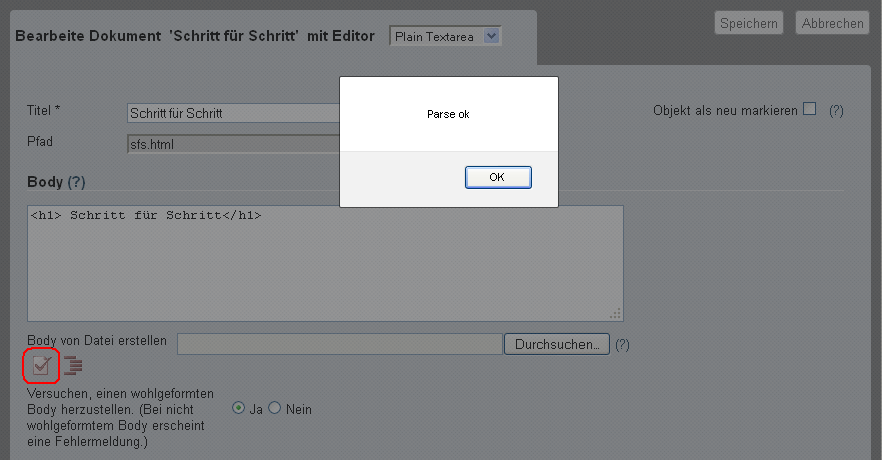
\includegraphics[width=0.9\textwidth]{./images/xmlvonbodytesten.png}
  \caption{Funktion �XML von \ximsterm{Body} testen�}
  \label{fig:xmlvonbodytesten}
\end{figure}

\begin{Hinweis}
  Mit der Funktion �Versuchen, einen wohlgeformten \ximsterm{Body}
  herzustellen� ver�ndert \otherterm{HTML-Tidy} die
  Whitespace-Informationen. Nach dem Speichern des Dokuments werden
  Einr�ckungen oder Umbr�che nicht mehr denen im Originaldokument
  entsprechen!
\end{Hinweis}

\paragraph{Schlagw�rter (Keywords)}
\label{keywords}

Die Liste der das Dokument beschreibenden \otherterm{Schlagw�rter}
soll durch Beistriche getrennt und in Kleinschreibung angef�hrt werden
(beispielsweise: \texttt{antrag, benutzungsantrag, studierende}). Bei
der Auswahl empfielt es sich, zu �berlegen, mit welchen Suchbegriffen
jemand versuchen k�nnte das fragliche Dokument zu finden. Die
gew�hlten Begriffe sollten m�glichst auch im Dokument selbst verwendet
worden sein.

\othertermdef{Schlagw�rter} scheinen bei ver�ffentlichten Dokumenten
als Metainformation auf. �ber die \otherterm{XIMS}-Suche kann gezielt
nach ihnen gesucht werden.

Mehr als zehn \otherterm{Schlagw�rter} anzugeben ist nicht sinnvoll.

\paragraph{Zusammenfassung (Abstract)}
\label{abstract}

Die Zusammenfassung soll eine kurze und pr�gnante Beschreibung des
Dokumentes enthalten. Sie scheint in der Regel unterhalb des Titels in
Suchergebnissen auf. Auch hier sollte man beim Erstellen versuchen,
sich in eine Person zu versetzen, die Informationen im fraglichen
Dokument ben�tigt.

Die Zusammenfassung sollte, wenn m�glich, relevante Stichw�rter aus
dem Dokument enthalten und nicht mehr als 150 Zeichen oder 30 W�rter
lang sein.

\paragraph{Objekt als neu markieren (Mark object as new)}
\label{markasnew}

\otherterm{XIMS} kann kann gezielt nach �als neu markierte Objekte�
suchen werden. Auch im Umgang mit Portlets und Filtern kann dieses
Attribut praktisch sein. Optisch ist die Markierung durch ein Icon
erkennbar (siehe Punkt \ref{new}).

\paragraph{Speichern (Save)}
\label{save}

Nach Klicken des �Speichern�-Buttons speichert \otherterm{XIMS} das
Dokument in der Datenbank. Sie gelangen anschlie�end zur
Standardansicht des Dokumentes.

\paragraph{Abbrechen (Cancel)}
\label{cancel}

Nach Klicken des �Cancel�-Buttons verwirft \otherterm{XIMS} alle
�nderungen. Sie gelangen anschlie�end zur \ximsterm{Containeransicht}
des Eltern-Containers.


\paragraph{\otherterm{Editieren} eines Dokuments}
\label{edit}

Ein bereits erstelltes Dokument zeigt sich nach einem Klick auf das
�Bearbeiten-Icon� in der Editiermaske, die im Wesentlichen der
Erstellen-Maske gleicht. Gleichzeitig wird der Schreibzugriff auf das
Dokument f�r Andere gesperrt.

Abh�ngig von der Editorwahl (TinyMCE oder Plain Textarea)
zeigt \otherterm{XIMS} eine entsprechende Editiermaske.\footnote{Am
  oberen Rand befindet sich ein Drop-Down-Menu f�r die Editorwahl.}

\begin{figure}[!ht]
  \centering
  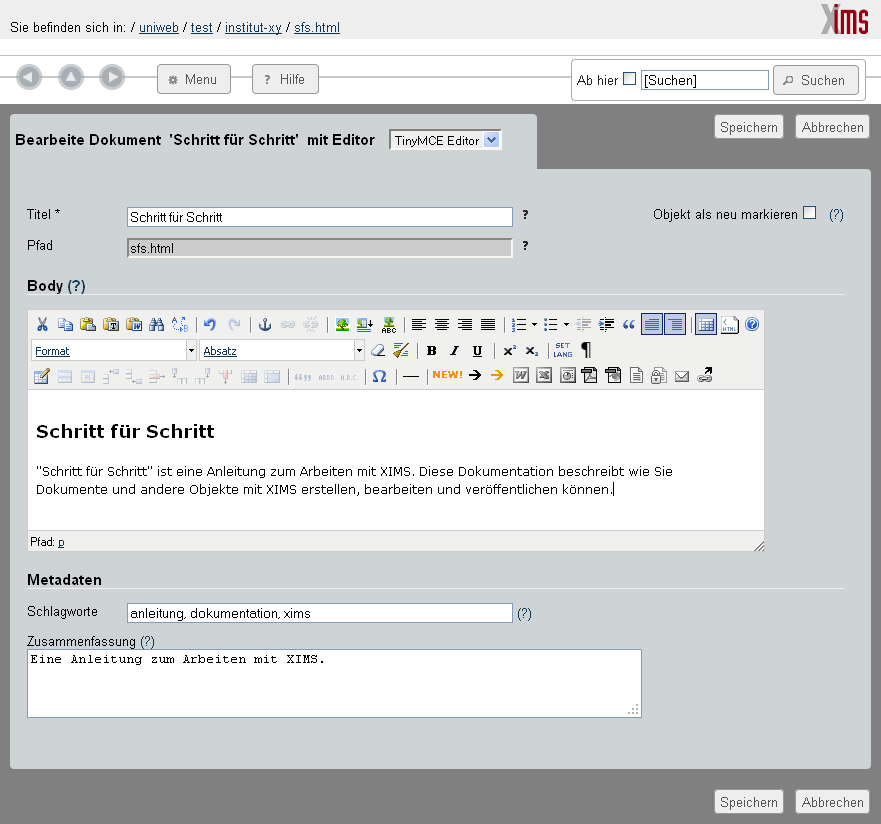
\includegraphics[width=0.9\textwidth]{./images/editdoktiny.png}
  \caption{Editieren eines XHTML Dokuments im TinyMCE-Editor}
  \label{fig:xhtmlintinymce}
\end{figure}


\begin{Hinweis}
  Ist ein Objekt publiziert, kann 
  %die \ximsterm{Location} 
  der Pfad
  nicht
  ver�ndert werden (siehe Abb.~\ref{fig:xhtmlintinymce}). Um 
  %die \ximsterm{Location} 
  den Pfad
  eines ver�ffentlichten Objekts ver�ndern zu
  k�nnen, muss dieses zuerst depubliziert werden.
\end{Hinweis}

Durch Klicken des �Speichern�-Buttons werden �nderungen gespeichert,
das Dokument entsperrt und man gelangt automatisch in die
Standardansicht des Dokuments zur�ck.

\subparagraph{Gesperrte Objekte}
\label{gesperrteobjekte}

Die Editiermaske darf nur �ber �Speichern� oder �Abbrechen� verlassen
werden, weil das Dokument sonst f�r Andere gesperrt bleibt.

\subsubsection{Verzeichnisse/Ordner (Folder)}
\label{ordner}

F�r das Erstellen eines Verzeichnisses ist nur die Eingabe 
%der \ximsterm{Location}
des Pfades
erforderlich. Wird kein Eintrag im Feld Titel gemacht, wird der 
%\ximsterm{Location}-Name
Pfad-Name
auch f�r das Titel-Feld �bernommen.

\begin{figure}[!ht]
  \centering
  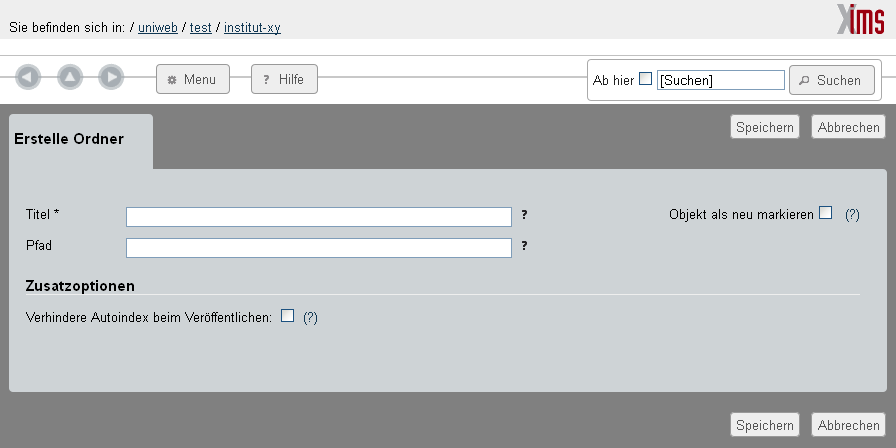
\includegraphics[width=\textwidth]{./images/erstellefolder.png}
  \caption{Erstellen eines Ordners}
  \label{fig:erstellefolder}
\end{figure}

%\paragraph{\ximsterm{Location}}
%Siehe Punkt~\ref{location}.

\paragraph{Titel}
Siehe Punkt~\ref{title}.

\paragraph{Pfad}
Siehe Punkt~\ref{location}.

\paragraph{Objekt als neu markieren}
Siehe Punkt~\ref{markasnew}.

\paragraph{Verhindere \ximstermdef{Autoindex} beim Ver�ffentlichen}
\label{autoindex}

Auf eine Anfrage nach einem Verzeichnis (z.\,B.: \url{http://www.uibk.ac.at/zid/}) liefert der
Webserver normalerweise ein sogenanntes Indexdokument aus. \otherterm{XIMS} kann beim
Ver�ffentlichen automatisch ein solches Dokument mit einer einfachen Liste des
Verzeichnisinhalts erstellen. Dieses Standardverhalten kann mit der Option
�Verhindere \ximsterm{Autoindex} beim Ver�ffentlichen� wenn n�tig unterbunden
werden.\footnote{Wir empfehlen, den \ximsterm{Autoindex} abzuschalten, falls Sie mehrsprachige Indexdokumente (z.\,B.:
  \nolinkurl{index.html.de} und \nolinkurl{index.html.en}) verwenden wollen, es kann sonst zu Fehlern bei der
  Sprachauswahl kommen.} In vielen F�llen ist es sinnvoll ein Indexdokument selbst zu erstellen; 
  %die \ximsterm{Location} 
  der Pfad
  muss \path{index.html} lauten, der Webserver verwendet es dann automatisch.

\begin{Hinweis}
  Ein Objekt mit 
  %der \ximsterm{Location} 
  dem Pfad \path{index.html} 
  %(z.\,B. \nolinkurl{index.html}) 
  wird vom Webserver gegen�ber dem automatisch
  erstellten Index vorgezogen, d.h. sobald ein Objekt mit 
  %der \ximsterm{Location} 
  dem Pfad 
  \path{index.html} in dem \ximsterm{Container}
  existiert, wird dieses Dokument ausgeliefert, auch wenn ein
  \ximsterm{Autoindex} erstellt wurde.
\end{Hinweis}

Ist in einem Verzeichnis kein Indexdokument vorhanden und publiziert, gibt der
Webserver auf eine Anfrage die Fehlermeldung
�Forbidden� zur�ck -- sinngem��: das Auf"|listen des Verzeichnisinhalts ist
verboten.\footnote{Die Dokumente darunter sind selbstverst�ndlich zug�nglich.}

\begin{Hinweis}
  Einfach nur zu verhindern dass ein Verzeichnis aufgelistet wird, ist
  kein taugliches Mittel, um Dokumente zu �verstecken� oder gar
  unzug�nglich zu machen!
\end{Hinweis}

\begin{figure}[!ht]
  \centering
  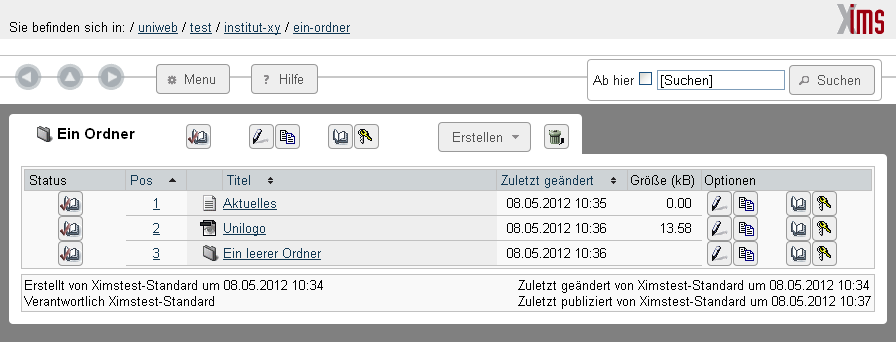
\includegraphics[width=\textwidth]{./images/ordnermitinhaltohneindex.png}
  \caption{\otherterm{XIMS} Ansicht eines Ordners mit Inhalt. Keines dieser Objekte hat 
  %die \ximsterm{Location}
   den Pfad
    \texttt{index.html}!}
  \label{fig:ordnerohneindex}
\end{figure}

\begin{figure}[!ht]
  \centering
  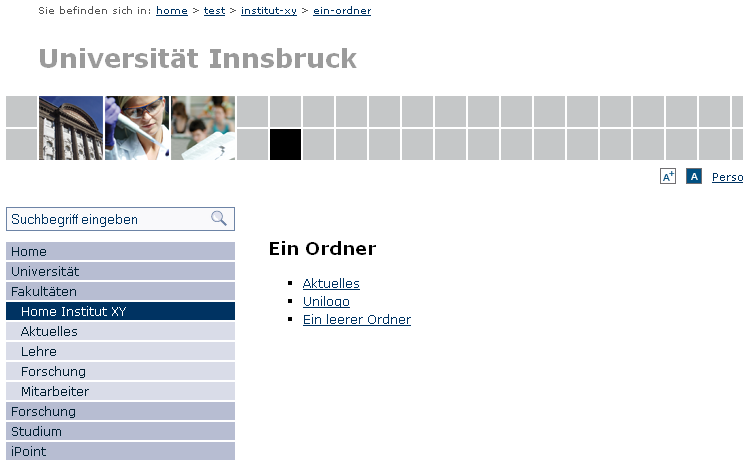
\includegraphics[width=\textwidth]{./images/ordnermitinhaltohneindex_publiziert.png}
  \caption{Die ver�ffentlichte Version desselben Ordners. Da kein Objekt mit 
  %der \ximsterm{Location}
  dem Pfad
   \texttt{index.html} enthalten ist, wird der Ordnerinhalt angezeigt. Die Darstellung im Bild
    zeigt den von \otherterm{XIMS} generierten \ximsterm{Autoindex}.}
  \label{fig:ordnerohneindexpubliziert}
\end{figure}

% Nur im Experten.Modus
%
%\paragraph{Zugriffsrechte erteilen}
%\label{zugriffsrechte}
%
%�ber diese Funktion k�nnen die \othertermdef{Berechtigung}en f�r das Objekt konfiguriert werden.
%\otherterm{XIMS} �vererbt� standardm��ig die Einstellungen von den Elternobjekten.
%
%\begin{description}
%\item[Nur mir selbst Rechte erteilen:]
%  Durch dieses Attribut kann das Objekt ausschlie�lich vom jeweiligen Besitzer
%  gelesen bzw. ver�ndert werden.
%\item[Zus�tzlich Leserechte f�r Mitglieder der Standard Rollen
%  erteilen:] (Grant VIEW privilege of your default roles) �ber dieses Attribut erhalten \otherterm{XIMS}-Standardrollen das Leserecht f�r dieses Objekt.
%\end{description}
%
%\begin{Hinweis}
%  Die Funktion �Zus�tzlich Leserechte f�r Mitglieder der Standard
%  Rollen erteilen� wird derzeit nicht verwendet!
%\end{Hinweis}

\paragraph{Editieren eines Verzeichnisses (Folders)}

Es k�nnen 
%die \ximsterm{Location},
der Pfad,
 der Titel und die Optionen �Objekt als neu
markieren� bzw. �Verhindere \ximsterm{Autoindex} beim Ver�ffentlichen� ge�ndert
werden. Au�erdem besteht die M�glichkeit die Anzahl der Eintr�ge pro Seite und die Kriterien f�r die standardm��ige
Sortierung der Kindobjekte des Verzeichnisses festzulegen (nach Position, Titel,
�nderungsdatum).
%Bitte beachten Sie an dieser Stelle Punkt \ref{gesperrteobjekte} �Gesperrte Objekte�.

\begin{figure}[!ht]
  \centering
  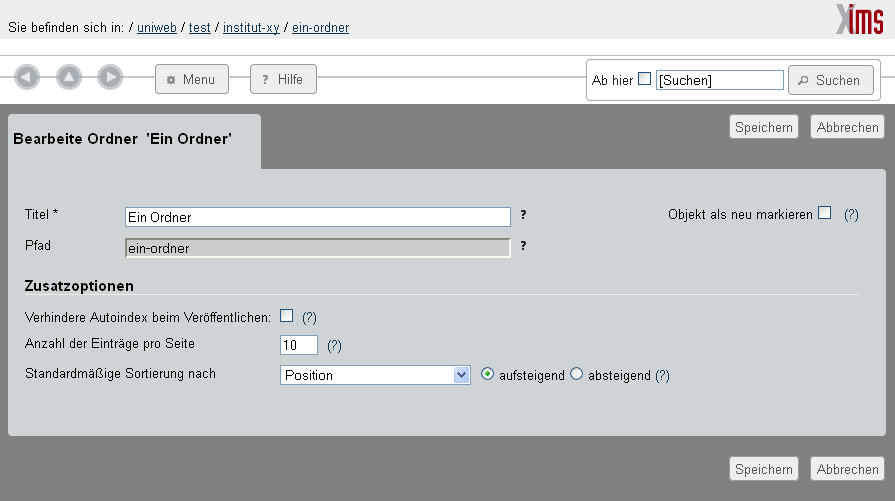
\includegraphics[width=\textwidth]{./images/edit-folder.png}
  \caption{Editieren eines Verzeichnisses (nicht publiziert)}
  \label{fig:editierefolder}
\end{figure}

\subsubsection{Bilder (Images)}
\label{bilder}

Um eine Bild-Datei (Image) in \otherterm{XIMS} zu erstellen, d.h. ein Bild vom lokalen Rechner zu importieren, kann man entweder die Durchsuchen-Funktion
verwenden oder den Dateipfad im lokalen Dateisystem direkt eingeben. �ber die
Durchsuchen-Funktion vermeidet man falsche Pfadangaben durch Tippfehler und
sie ist der komfortablere Weg um den Pfad zur gew�nschten Bild-Datei zu
generieren (z.\,B.: \path{D:\Bilder\Beispielbilder\Sonnenuntergang.jpg}).

\begin{figure}[!ht]
  \centering
  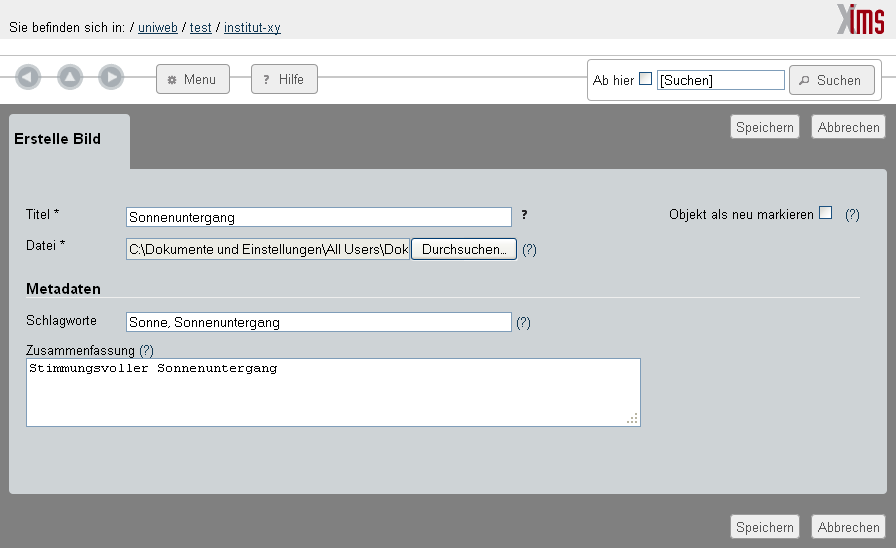
\includegraphics[width=\textwidth]{./images/create-image.png}
  \caption{Erstellen einer Bild-Datei in \otherterm{XIMS}}
  \label{fig:erstellebild}
\end{figure}

\paragraph{Titel}
Der Titel (in unserem Beispiel Sonnenaufgang) entspricht dem Namen des Bildes,
unter dem das Bild in der \ximsterm{Containeransicht} aufscheint.

\paragraph{Datei (File)}
\label{datei}
Dieses Eingabefeld dient zur Angabe des Verzeichnispfades unter dem das Bild / die Datei am lokalen
Rechner zu finden ist (in unserem Beispiel unter \path{D:\Bilder\Beispielbilder\Sonnenuntergang.jpg}.

Der Durchsuchen-Button erleichtert die Angabe des absoluten Dateipfades durch
�ffnen eines Dateiauswahl-Dialoges.

\paragraph{ZIP-Archive}
\label{zip-archives}
Wollen Sie mehrere Bilder im gleichen Verzeichnis neu erstellen, k�nnen Sie diese vorab in ein Archiv im ZIP-Format packen und anschlie�end in einem Arbeitsschritt in \otherterm{XIMS} hochladen. W�hlen Sie dazu wie bei einem einzelnen Bild den ">Durchsuchen"<-Button neben dem Datei-Feld und w�hlen Sie nun eine ZIP-Datei von Ihrem lokalen Rechner aus. Sobald der Dialog zum Datei hochladen geschlossen wurde, erscheinen nun zwei weitere Optionen

\begin{itemize}
	\item Inhalte entpacken: Best�tigen Sie diese Option um die Bilder in Ihr XIMS-Verzeichnis zu entpacken. Andernfalls w�rde die ZIP-Datei selbst hochgeladen und nicht die darin enthaltenen Bilder. 
	\item �berschreibe vorhandene Dateien beim entpacken. Wenn Sie diese Option aktivieren, werden bereits vorhandene Bilddateien mit 
	%der gleichen Location 
	dem gleichen Pfad 
	durch die neuen ersetzt.
\end{itemize}

Als 
%Location
Pfad
 und Titel f�r die hochgeladenen Dateien wird automatisch der Dateiname des Bildes, den es auf Ihrem lokalen Rechner hat, gesetzt.

\begin{Hinweis}
  Wenn Sie mehrer Bilder in einem ZIP-Archiv zusammenfassen um es in XIMS hochzuladen, achten Sie darauf, dass nur einzelne Bilddateien - keine Ordner oder Unterordner gepackt werden.
\end{Hinweis}

\paragraph{Schlagw�rter}

Siehe Punkt \ref{keywords}

\paragraph{Zusammenfassung}

Siehe Punkt \ref{abstract}

%\paragraph{Zugriffsrechte erteilen}
%Siehe Punkt \ref{zugriffsrechte}

\paragraph{Speichern}
\label{upload}
Das Klicken des �Speichern�-Buttons speichert die ausgew�hlte Datei im \otherterm{XIMS} und
man wird zur \ximsterm{Containeransicht} weitergeleitet.

\paragraph{Abbrechen}
Siehe Punkt \ref{cancel}

\paragraph{Editieren eines Bildes (Image)}
\label{edit-image}
Es k�nnen Titel, \otherterm{Schlagw�rter}, Zusammenfassung und bei unver�ffentlichten Bildern der Pfad der Datei ge�ndert
werden. Soll die Datei durch eine andere ersetzt werden, kann man mit
Hilfe des �Durchsuchen�-Dialoges den Pfad zur neuen Datei angeben bzw.
diesen direkt ins Eingabefeld eintippen. Will man lediglich den Titel
editieren, so kann das Feld �Bild ersetzen� leer bleiben.

\subsubsection{Dateien (Files)}
\label{dateien}
Um eine bin�re Datei (MS-Word Dokument, PDF-Datei, etc.) zu erstellen, d.h. die
Datei vom lokalen Rechner zu importieren, kann man entweder die
Durchsuchen-Funktion verwenden oder den Dateipfad im lokalen Dateisystem direkt
eingeben. �ber die Durchsuchen-Funktion vermeidet man falsche Pfadangaben
durch Tippfehler und sie ist der komfortablere Weg um den Pfad zur gew�nschten
Datei zu generieren (z.\,B.: \path{G:\docs\anmeldung.pdf}).

% wie bei image
%
%\begin{figure}[!ht]
%  \centering
%  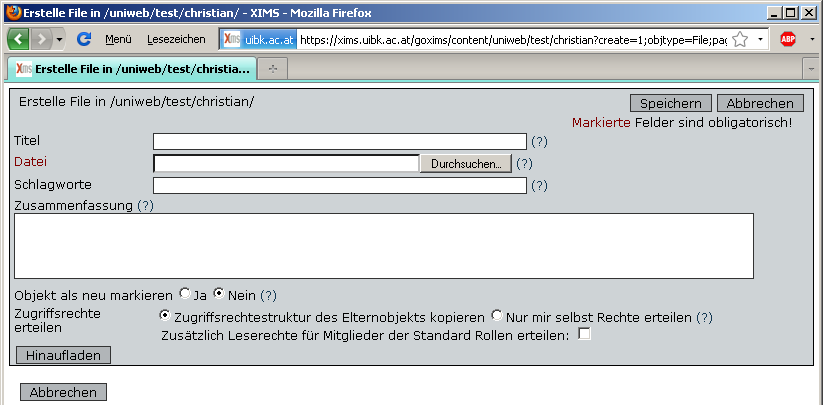
\includegraphics[width=\textwidth]{./images/create-file.png}
%  \caption{Erstellen einer Datei}
%  \label{fig:erstelledatei}
%\end{figure}

\paragraph{Titel}
Siehe Punkt \ref{title}

\paragraph{Datei}
Siehe Punkt \ref{dateien}

\paragraph{ZIP-Archive}
Siehe Punkt \ref{zip-archives}

\paragraph{Schlagw�rter}
Siehe Punkt \ref{keywords}

\paragraph{Zusammenfassung}
Siehe Punkt \ref{abstract}

%\paragraph{Zugriffsrechte erteilen}
%Siehe Punkt \ref{zugriffsrechte}

\paragraph{Speichern}
Siehe Punkt \ref{upload}

\paragraph{Abbrechen}

Siehe Punkt \ref{cancel}

\paragraph{Editieren einer Datei (File)}
Es wird auf Punkt \ref{edit-image} verwiesen, da alle wesentlichen Editierm�glichkeiten
�bereinstimmen.

% wie bei image
%
%\begin{figure}[!ht]
%  \centering
%  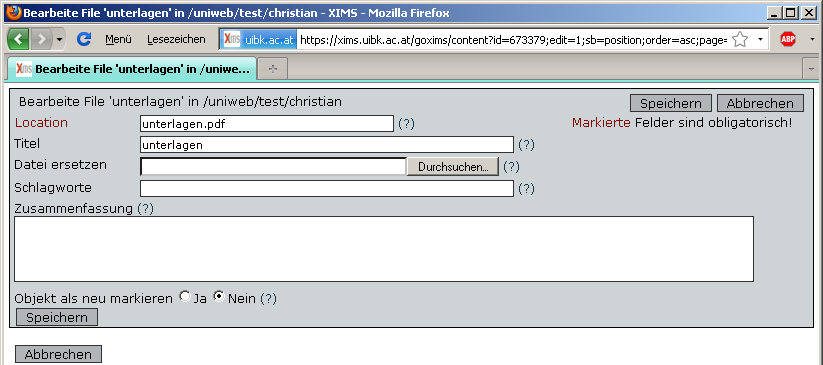
\includegraphics[width=\textwidth]{./images/edit-file.png}
%  \caption{Editieren einer Datei (nicht publiziert)}
%  \label{fig:editieredatei}
%\end{figure}

\subsubsection{\ximstermdef{URLLink}s}
\label{urllinks}

�ber den \ximsterm{Objekttyp} \ximsterm{URLLink} k�nnen sowohl externe (d.h. Links au�erhalb
der Dom�ne \url{http://www.uibk.ac.at}) als auch interne Links erstellt
werden. Hinzu kommt, dass diesem Objekttyp bei der Erstellung von
\ximsterm{DepartmentLinks} eine besondere Rolle zukommt (siehe Punkt \ref{deplinks}). Bei internen Links ist zu beachten, dass diese absolut zum \ximsterm{SiteRoot} anzugeben sind (i.d.R. absolut zu \path{/uniweb}). Alternativ kann
auch die offizielle \otherterm{URL} der Seite (z.\,B. \url{http://www.uibk.ac.at/zid}),
welche verlinkt werden soll, angegeben werden. Externe Links m�ssen
zwingend mit dem \nolinkurl{http://}- bzw. \nolinkurl{https://}-Prefix angegeben werden.

\paragraph{\ximsterm{Location}}
Die \ximsterm{Location} bei \ximsterm{URLLink} Objekten wird anders gehandhabt als 
%die \ximsterm{Location}
der Pfad 
anderer Objekte. Bei \ximsterm{URLLink} Objekten beschreibt die \ximsterm{Location} den Pfad zum Objekt auf welches verwiesen wird.
Grunds�tzlich sind dieselben Regeln wie bei URLs �blich zu beachten. Jeder nach RFC 2396 g�ltiger URI ist zul�ssig. Mit dem ">Ziel suchen"<-Button k�nnen Sie innerhalb von XIMS nach dem Zielobjekt suchen (siehe Abbildung \ref{fig:urlzielsuchen}) und so falsche Verlinkungen durch Tippfehler vermeiden.

\begin{figure}[!ht]
  \centering
  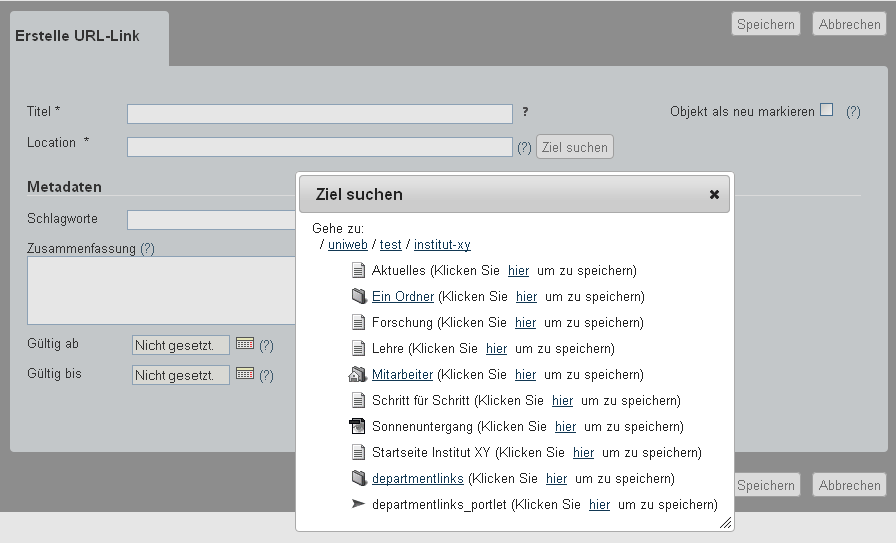
\includegraphics[width=\textwidth]{./images/urllink-ziel-suchen.png}
  \caption{">Ziel suchen"<-Dialog}
  \label{fig:urlzielsuchen}
\end{figure}

\paragraph{Titel}
Siehe Punkt \ref{title}

\paragraph{Schlagw�rter}
Siehe Punkt \ref{keywords}

\paragraph{Zusammenfassung}
Siehe Punkt \ref{abstract}

%\paragraph{Zugriffsrechte erteilen}
%Siehe Punkt \ref{zugriffsrechte}

\paragraph{G�ltig ab / G�ltig bis}
Bei URL-Links k�nnen Sie durch setzen der ">G�ltig ab"<- und ">G�ltig bis"<-Attribute die G�ltigkeit beschr�nken. Klicken Sie auf das Kalender-Icon neben dem Eingabefeld, �ffnet sich ein Kalender als Popup, in dem Sie bequem Datum und Uhrzeit setzen k�nnen. Sind die G�ltigkeitsattribute nicht bestimmt, ist der URL-Link ab sofort bzw. unbegrenzt g�ltig. 

\paragraph{Speichern}
Siehe Punkt \ref{save}

\paragraph{Abbrechen}
Siehe Punkt \ref{cancel}

\paragraph{Editieren eines URL-Links}
Hier wird auf Punkt \ref{edit} verwiesen, da alle wesentlichen Editierm�glichkeiten
�bereinstimmen.

\subsubsection{Portlets}
\label{portlets}

Ein \ximstermdef{Portlet} kann als eine spezielle Sicht auf eine bestimmte Datenmenge bezeichnet
werden. Bei Webseiten erscheinen Portlets normalerweise in Form von Boxen neben
dem eigentlichen Inhalt der Seite. Eine Seitennavigation kann zum Beispiel ein Portlet darstellen (siehe dazu auch Punkt \ref{deplinks}).

\begin{figure}[!ht]
  \centering
  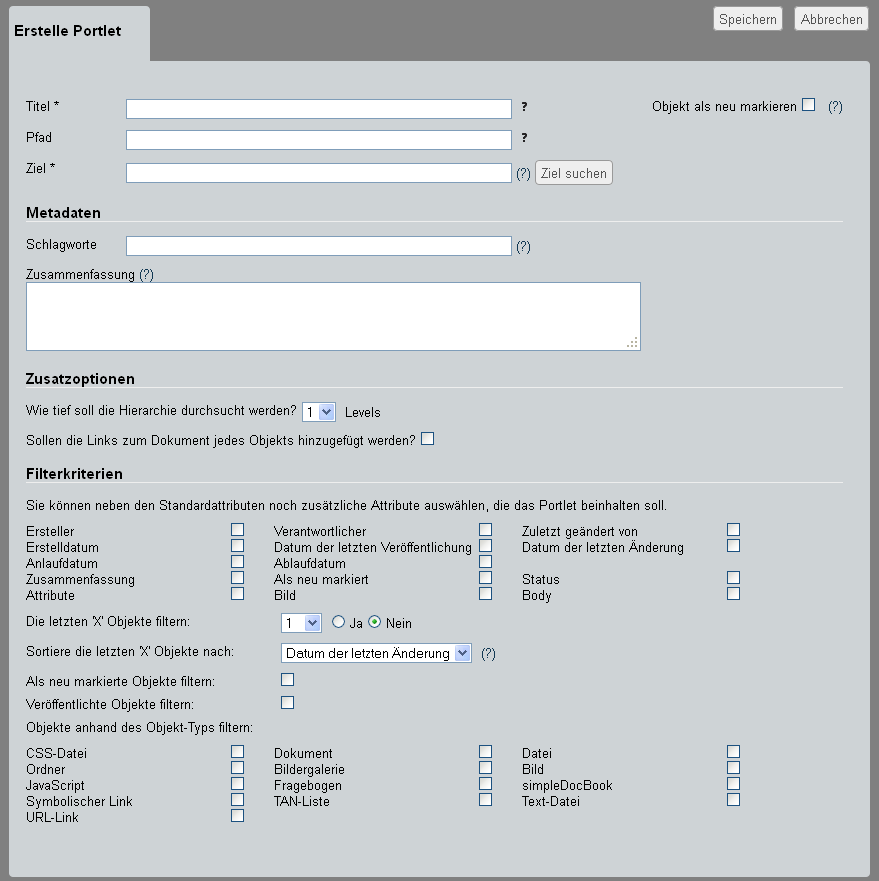
\includegraphics[width=\textwidth]{./images/erstelleportlet.png}
  \caption{Erstellen eines Portlets}
  \label{fig:erstelleportlet}
\end{figure}

\paragraph{Titel}
Siehe Punkt \ref{title}

%\paragraph{\ximsterm{Location}}
\paragraph{Pfad}
Siehe Punkt \ref{location}

\paragraph{Ziel (Target)}
Als Ziel wird der Pfad jenes Verzeichnisses bzw. jener Datenmenge angegeben, auf
das bzw. die das \ximsterm{Portlet} seine spezielle Sicht richten soll.
Die �Ziel Suchen� (Browse for Target)-Funktionalit�t erleichtert das exakte
Bestimmen dieses Pfades.

\begin{Hinweis}
  �ber ein \ximsterm{Portlet} kann zum Beispiel eine Box mit einer
  Linkliste als Inhalt einfach erstellt werden. \otherterm{XIMS}
  durchsucht hierf�r den Inhalt eines \ximsterm{Container}s (z.\,B.
  eines Verzeichnisses) und listet den entsprechenden Inhalt (z.\,B.
  eine Reihe von Dokumenten), dargestellt als Liste mit Links
  verweisend auf die entsprechenden Dokumente, auf.
\end{Hinweis}

%\paragraph{Zus�tzlich Leserechte f�r Mitglieder der Standard Rollen erteilen}
%Siehe Punkt \ref{zugriffsrechte} sowie Punkt \ref{rollenverwaltung}

\paragraph{Zus�tzliche Einstellm�glichkeiten f�r \ximsterm{Portlet}s}
Portlets sind ein m�chtiges Werkzeug von \otherterm{XIMS}. Sie schaffen zus�tzlich zur
Auf"|listung der Objekttitel eine Reihe anderer M�glichkeiten, z.\,B. k�nnen
Containerinhalte gefiltert nach speziellen Attributen bzw. \ximsterm{Objekttyp}en dargestellt
werden. F�r genauere Informationen bez�glich \ximsterm{Portlet}s wird auf die \otherterm{XIMS}-Schulungen
bzw. den \otherterm{XIMS}-Support verwiesen.

\paragraph{Editieren eines \ximsterm{Portlet}s}
Siehe Punkt \ref{erstelleneditieren}

\subsubsection{\ximstermdef{DepartmentRoot}s}
\label{departmentroots}
Der Begriff �DepartmentRoot� beschreibt die Startseite einer Organisationseinheit
und entspricht einer erweiterten Version eines \otherterm{XIMS}-Ordners mit besonderen
Eigenschaften. Ein �DepartmentRoot� definiert einige Eigenschaften, die auf
�Kinderobjekte� (untergeordnete Webseiten einer Organisationseinheit) weitervererbt
werden. Zu diesen Eigenschaften z�hlen �\ximsterm{Portlet}s� der Organisationseinheit -- wie
zum Beispiel das �DepartmentLink-Portlet�, ein f�r die Organisationseinheit bzw. f�r
das Institut spezifisches Bild (�DepartmentImage�), wie auch der �Department Titel�
bzw. der �Department Infotext� oder ein f�r die Organisationseinheit bzw. f�r das
Institut spezifisches \otherterm{XSLT}-Stylesheet f�r eine angepasste Darstellung
ver�ffentlichter Seiten.

\begin{Hinweis}
  Der Objekttyp DepartmentRoot ist standardm��ig nicht f�r alle Nutzer freigeschalten. Wenn Sie mit DepartmentRoots arbeiten wollen und dieser Objekttyp nicht im Erstellen-Men� gelistet ist, wenden Sie sich an den Xims-Support.
\end{Hinweis}

Abbildung~\ref{fig:departmentrootzid} zeigt wie ein individualisierter DepartmentRoot mit
�DepartmentLinks�, �DepartmentImage�, �Department Titel�, �Department Infotext�
und �DepartmentSpeziallinks� aussehen k�nnte. Die individualisierten Elemente sind
auch auf allen untergeordneten Webseiten der Organisationseinheit wirksam.

\begin{itemize}
\item {[1] Department Titel}
\item {[2] Department Info}
\item {[3] DepartmentImage}
\item {[4] DepartmentLinks}
\item {[5] DepartmentSpeziallinks}
\end{itemize}

\begin{figure}[!ht]
  \centering
  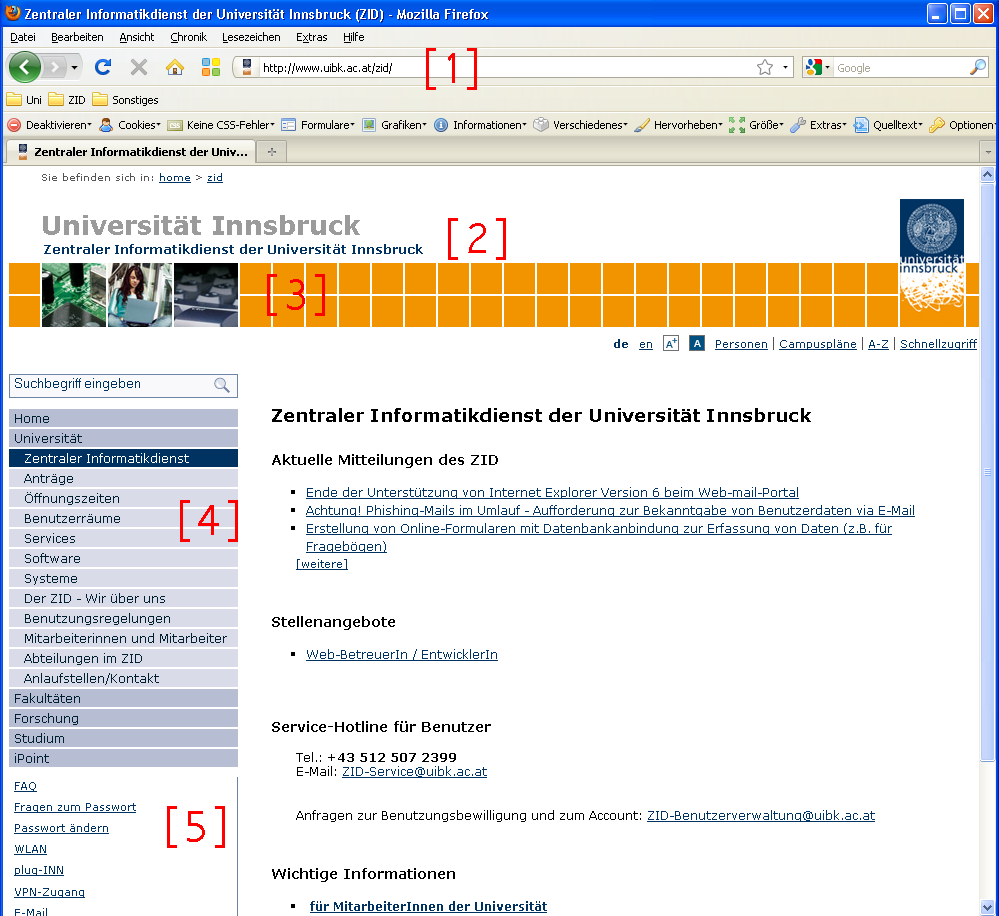
\includegraphics[width=\textwidth]{./images/departmentroot-zid.png}
  \caption{DepartmentRoot mit adaptierbaren Elementen}
  \label{fig:departmentrootzid}
\end{figure}

\paragraph{Erstellen eines \ximsterm{DepartmentRoot}-Objekts}

Ist noch kein \ximsterm{DepartmentRoot}-Container vorhanden bzw. vom
\otherterm{XIMS}-Support eingerichtet worden, muss das \ximsterm{DepartmentRoot}"-Objekt
erstellt werden. Dies erfolgt in gleicher Weise wie etwa das Erstellen
eines Verzeichnisses (siehe Punkt \ref{erstelleneditieren}).

\begin{Hinweis}
  Eine besondere Bedeutung hat im \ximsterm{DepartmentRoot}-Kontext
  die Zusammenfassung (Abstract). Mit Hilfe des Zusammenfassung Feldes
  kann der �Department Infotext� gesetzt werden. Umgeben mit dem
  \texttt{<span>}-Tag und in Verbindung mit dem lang-Attribut
  repr�sentiert der so gekapselte Text den �Department Infotext� in
  deutscher bzw. englischer Sprache.
\end{Hinweis}

\begin{figure}[!ht]
  \centering
  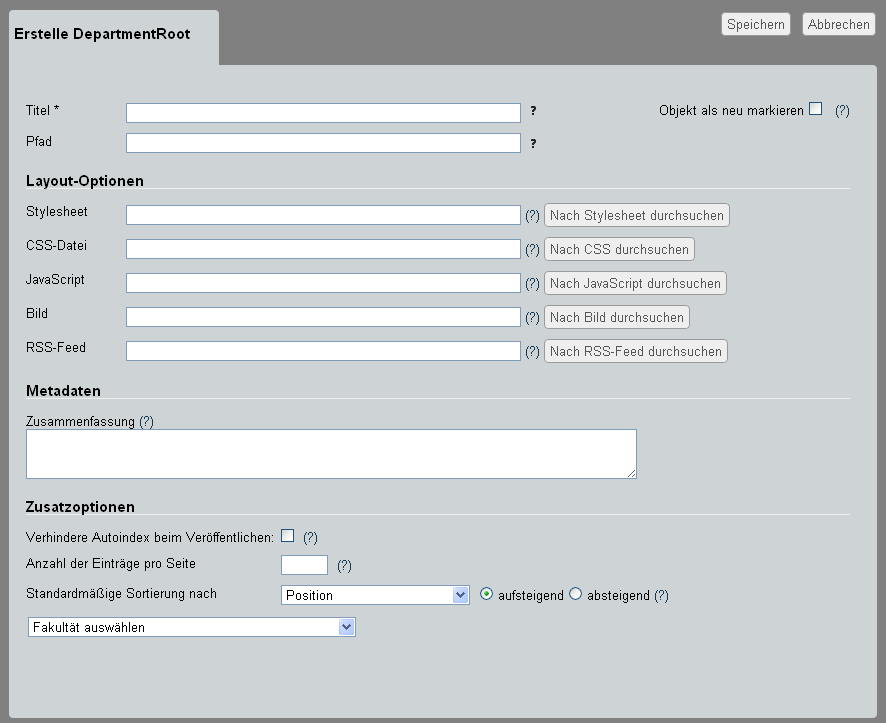
\includegraphics[width=\textwidth]{./images/create-departmentroot.png}
  \caption{Erstellen eines \ximsterm{DepartmentRoot}}
  \label{fig:erstellendepartmentroot}
\end{figure}

\paragraph{Stylesheet}
Dem \ximsterm{DepartmentRoot} kann hier ein spezielles Stylesheet zugewiesen werden.

\paragraph{CSS}
Dem \ximsterm{DepartmentRoot} kann hier ein spezielles CSS zugewiesen werden.

\paragraph{JavaScript}
Dem \ximsterm{DepartmentRoot} kann hier ein spezielles JavaScript zugewiesen werden.

\paragraph{Bild}
Dem \ximsterm{DepartmentRoot} kann hier ein spezielles \ximsterm{DepartmentImage} zugewiesen
werden. Siehe dazu Punkt \ref{depimg}.

\paragraph{RSS-Feed}

Dem \ximsterm{DepartmentRoot} kann hier ein spezieller RSS-Feed zugewiesen werden.

%\paragraph{Ausblenden der 3. Spalte f�r dieses \ximsterm{DepartmentRoot}}
%
%Ist diese Option aktiviert, wird die rechts �u�erste Spalte des Unidesigns (Quicklinks,
%Service, ...) ausgeblendet.

\paragraph{Editieren eines \ximsterm{DepartmentRoot}s}

Zus�tzlich zu den Einstellungen die man beim Erstellen eines \ximsterm{DepartmentRoot}
machen kann, kann man beim Editieren dem \ximsterm{DepartmentRoot} \ximsterm{Portlet}s hinzuf�gen.
N�here Informationen dazu finden sich unter Punkt \ref{depnav}.

\subsubsection{\ximstermdef{sDocBookXML} Objekte}
\label{sdocbookxml}

\begin{quotation}
  �DocBook is an XML/SGML vocabulary particularly well suited to books and papers
  about computer hardware and software (though it is by no means limited to these
  applications).� Homepage des DocBook Technical Committee
\end{quotation}

Unter DocBook versteht man XML-Dokumente, welche den Regeln einer
bestimmten DTD (Document Type Definition) folgen. Es dient dazu,
strukturierte Dokumente mit Hilfe von XML zu schreiben. Docbook XML
eignet sich besonders f�r B�cher und Artikel �ber
Computerhardware/-software sowie sonstige technische Dokumentationen.
Docbook XML verfolgt das Konzept, Dokumente unabh�ngig vom sp�ter
publizierten Medium (z.\,B. Internetseite, gedrucktes Buch) zu
erstellen. F�r die sp�tere Konvertierung in das entsprechende
Endformat wird \otherterm{XSLT} verwendet. In \otherterm{XIMS} k�nnen Simplified Docbook XML
Objekte (\ximsterm{sDocBookXML}) erstellt werden. Simplified DocBook XML bzw. die
entsprechende DTD l�sst mit ca. 100 XMLElementen weniger Elemente als
DocBook XML zu. Simplified Docbook XML (\ximsterm{sDocBookXML}) ist eine also
Untermenge von DocBook XML, welche besonders f�r kleinere Dokumente
(Artikel, White Papers u.�.) gedacht ist.

\begin{figure}[!ht]
  \centering
  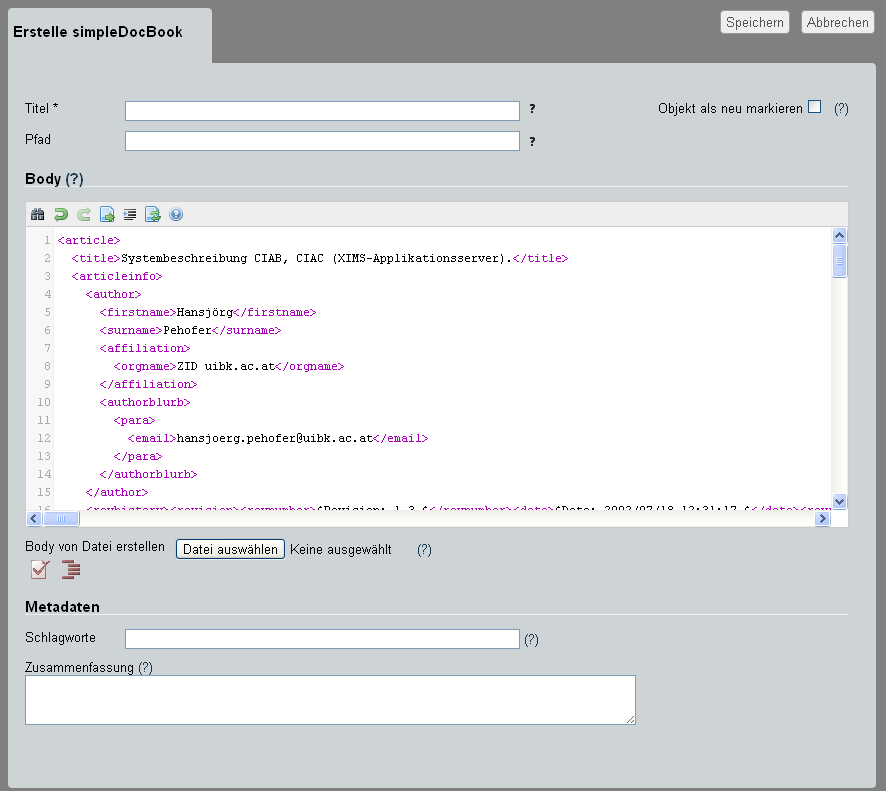
\includegraphics[width=\textwidth]{./images/create-sdocbookxml.png}
  \caption{Erstellen eines Simplified Docbook XML Objekts}
  \label{fig:erstelledocbookxml}
\end{figure}

%\paragraph{\ximsterm{Location}}
%Siehe Punkt \ref{location}

\paragraph{Titel}
Siehe Punkt \ref{title}

\paragraph{Pfad}
Siehe Punkt \ref{location}

\paragraph{Body}

Anders als beim Erstellen eines Dokuments gibt es hier keinen WYSIWYG-Editor
zum Schreiben eines \ximsterm{sDocBookXML}-Artikels. Daher empfiehlt es sich, das
\ximsterm{sDocBookXML}-Dokument mit Hilfe eines externen Editors zu erstellen und den
\otherterm{Quellcode} anschlie�end in das Body-Textfeld zu kopieren.

Ein externer Editor mit Unterst�tzung f�r \ximsterm{sDocBookXML} ist zum Beispiel XMLmind.
Dieser steht zum kostenlosen Download zur Verf�gung. Ein Tutorial zu XMLmind ist
dort ebenfalls verf�gbar.

Grunds�tzlich gilt, dass ein \ximsterm{sDocBookXML}-Dokument zum einen in wohlgeformtem
XML vorliegen muss und zum anderen keine Deklarationen oder Processing
Instructions (PIs) im \ximsterm{Body} des \ximsterm{sDocBookXML}-Dokuments aufscheinen d�rfen. Alle
Elemente von \ximsterm{sDocBookXML}-Dokumenten m�ssen zwingend Kind-Elemente des
Wurzelelements \texttt{<article>} sein.

\begin{Hinweis}
  Sollte das \ximsterm{sDocBookXML} Dokument wohlgeformt sein, jedoch
  Elemente enthalten, welche nicht in der Simplified DocBook XML DTD
  definiert sind, so werden diese Elemente zwar von \otherterm{XIMS}
  �akzeptiert�, jedoch in der ver�ffentlichten Version nicht
  dargestellt. Solche Elemente existieren dann nur im Quelldokument im
  \otherterm{XIMS}. Aus diesem Grund sollte man nur valide
  \ximsterm{sDocBookXML}-Dokumente ins \otherterm{XIMS} einpflegen.
\end{Hinweis}

\paragraph{Schlagw�rter}

Siehe Punkt \ref{keywords}

\paragraph{Zusammenfassung}

Siehe Punkt \ref{abstract}

%\paragraph{Zugriffsrechte erteilen}
%Siehe Punkt \ref{zugriffsrechte}

\paragraph{Speichern}

Siehe Punkt \ref{save}

\paragraph{Abbrechen}

Siehe Punkt \ref{cancel}

%\begin{figure}[!ht]
%  \centering
%  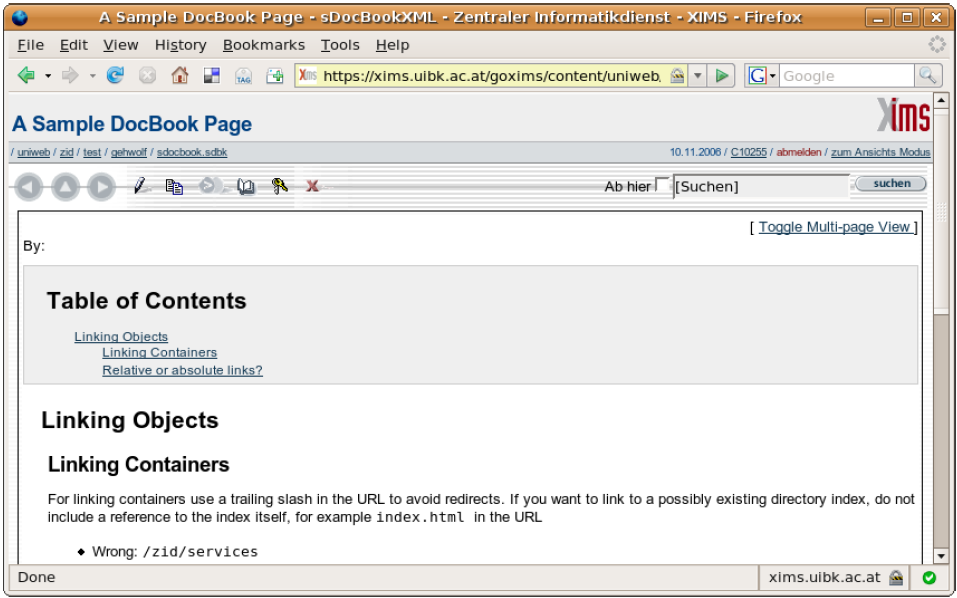
\includegraphics[width=\textwidth]{./images/sdocbookxmlerstellt.png}
%  \caption{Das erstellte \ximsterm{sDocBookXML} Objekt in der Vollansicht}
%  \label{fig:sdocbookxmlerstellt}
%\end{figure}

\paragraph{Editieren eines \ximsterm{sDocBookXML} Objekts}

Siehe Punkt \ref{erstelleneditieren}. 

\subsubsection{Bildergalerie (\ximstermdef{Gallery})}
\label{gallery}

Der Objekttyp Bildergalerie ist prinzipiell eine besondere Form eines Ordners. In einer Bildergalerie
k�nnen Bilder abgelegt werden, die dann mittels Javascript als Bildergalerie dargestellt werden.
Standardm��ig wird die Bildergalerie im XIMS in der Container Ansicht angezeigt. Wie von Ordner und 
Departmentroot gewohnt k�nnen von hier aus �ber das Erstellen-Menu weitere Bilder hinzugef�gt werden. 
Rechts neben dem Erstellen-Menu befindet sich ein Link zur Vorschau-Ansicht.
In der Vorschau-Ansicht (siehe Abbildung \ref{fig:gallery-preview}) werden alle im Gallery-Container 
ver�ffentlichten Bilder als Bildergalerie (wie nach der Ver�ffentlichung) angezeigt. Auch von hier aus 
lassen sich neue Bilder erstellen.
Um innerhalb der Bildergalerie zu navigieren gibt es mehrer M�glichkeiten: Durch Klick auf ein Thumbnail 
wird jeweilige Bild in der definierten Gr��e dargestellt. Oberhalb des gerade betrachteten Bildes 
befinden sich Navigationspfeile, durch die man zum jeweils vorherigen oder n�chsten Bild gelangt. Zudem f�hrt
ein Klick auf das Hauptbild zur Anzeige des jeweils n�chsten.
\begin{figure}[!ht]
  \centering
  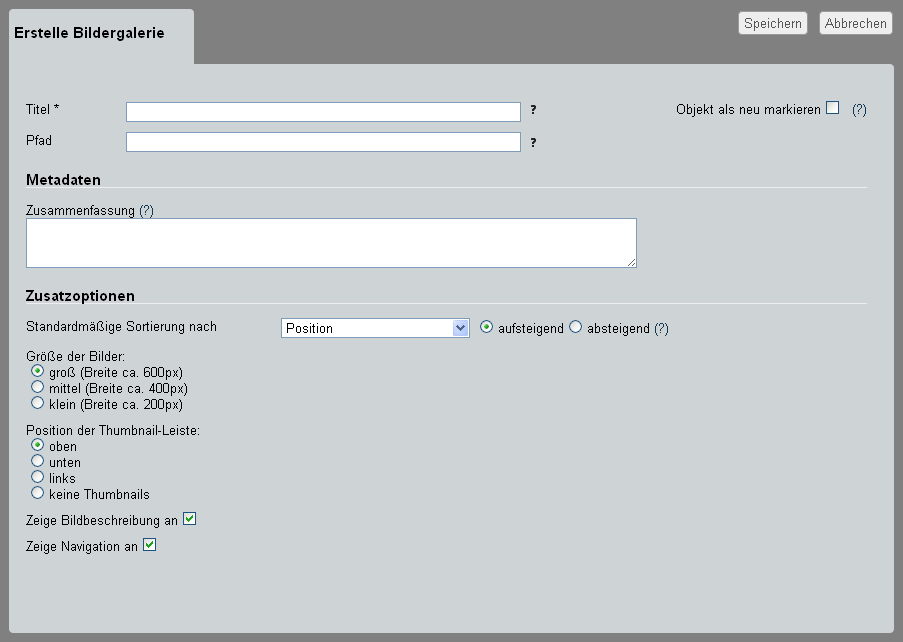
\includegraphics[width=\textwidth]{./images/create-gallery.png}
  \caption{Erstellen einer \ximsterm{Gallery}}
  \label{fig:create-gallery}
\end{figure}

%\paragraph{\ximsterm{Location}}
%Siehe Punkt \ref{location}.

\paragraph{Titel}
Siehe Punkt \ref{title}. Der Titel erscheint als �berschrift �ber der Bildergalerie.

\paragraph{Pfad}
Siehe Punkt \ref{location}.

\paragraph{Zusammenfassung}
Siehe Punkt \ref{abstract}. Die Zusammenfassung l�sst sich f�r eine kurze Beschreibung der Bildergalerie 
nutzen. Hier eingegebener Text erscheint unter der �berschrift.

\paragraph{Objekt als neu markieren}
Siehe Punkt \ref{abstract}.

\paragraph{Sortierung}
Wie bei einem Ordner kann hier die Sortierung der enthaltenen Objekte festgelegt und dabei zwischen 
Position, Titel und �nderungsdatum gew�hlt werden. Die gew�hlte Sortierung wird sowohl f�r die Container-Ansicht 
als auch f�r die Galerie-Darstellung �bernommen. 

\paragraph{Gr��e der Bilder}
F�r die Darstellung der Bilder gibt es drei Auswahlm�glichkeiten bez�glich der Gr��e: gro� (Breite ca. 600px), mittel (Breite ca. 400px) oder klein (Breite ca. 200px). Das aktuell betrachtete Bild wird auf die gew�hlte Breite skaliert, die H�he proportional angepasst (keine Verzerrung). Kleine Bilder werden entsprechend vergr��ert und k�nnen �pixelig� werden. Die Gr��e sollte also entsprechend der Qualit�t der Ausgangsbilder gew�hlt werden.

\paragraph{Position der Thumbnails}
Die Position der Thumbnails relativ zum aktuell betrachteten Bild. Die Auswahlm�glichkeiten sind oben, unten, links und keine Thumbnails.

\paragraph{Bildbeschreibung}
Die Bildbeschreibung wird aus der Zusammenfassung eines Bilds generiert und erscheint dann jeweils unter dem aktuell betrachteten Bild. Auf Wunsch kann die Beschreibung ausgeblendet werden. Dies gilt f�r alle Bilder einer Bildergalerie.

\paragraph{Navigation}
Die Navigation erzeugt Links zum jeweils vorherigen und n�chsten Bild. Sie befindet sich immer oberhalb des aktuell betrachten Bildes und kann ausgeblendet werden.

%\paragraph{Zugriffsrechte}
%Siehe Punkt \ref{zugriffsrechte}.

\begin{figure}[!ht]
  \centering
  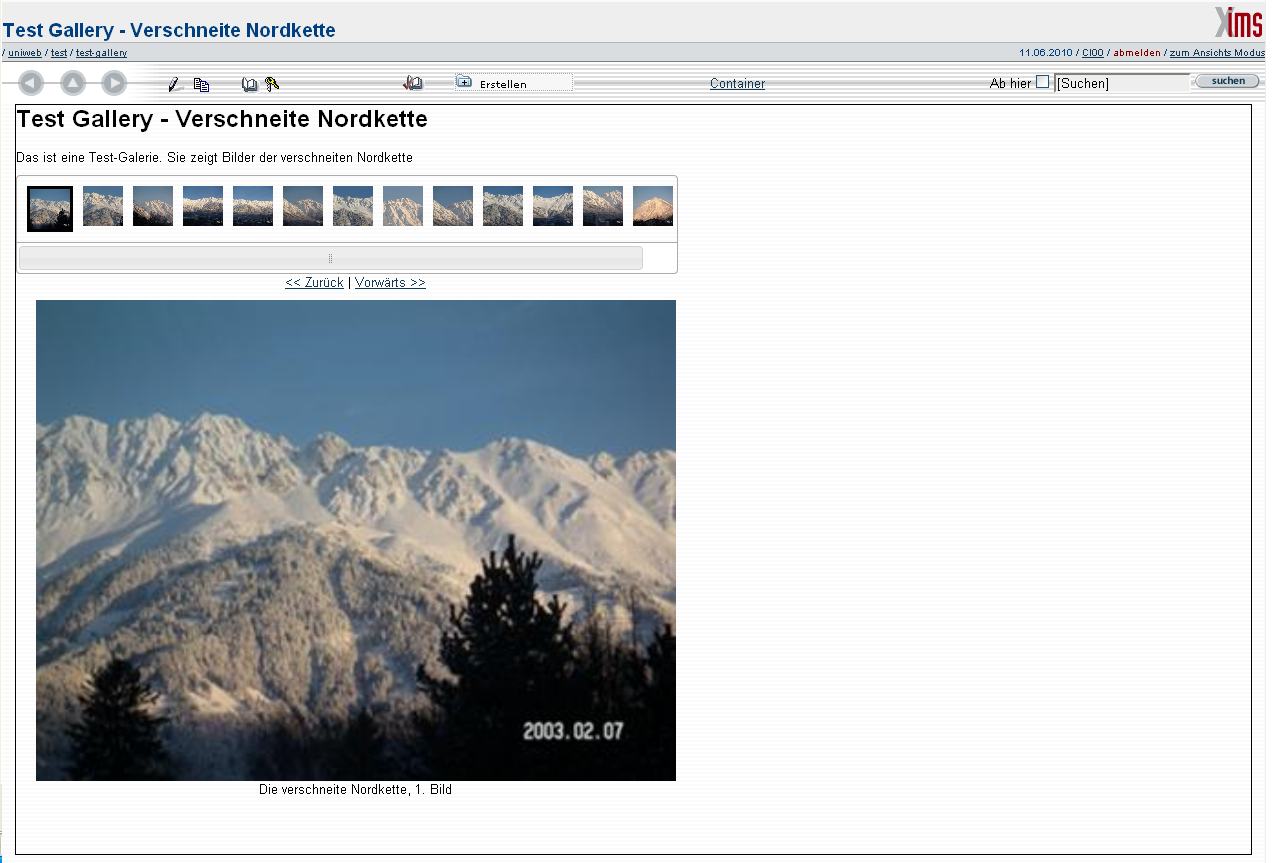
\includegraphics[width=\textwidth]{./images/gallery-preview.png}
  \caption{Die \ximsterm{Gallery} in der Vorschauansicht, hier mit gro�en Bildern, Thumbnail-Leiste oben, eingeblendeter Navigation und Bildbeschreibung}
  \label{fig:gallery-preview}
\end{figure}

\subsection{Objekte l�schen und �Papierkorb�}
\label{delete}

Objekte k�nnen mit dem ">L�schen"<-Icon gel�scht werden, wenn sie unver�ffentlicht sind
und die entsprechenden Privilegien in der ACL vergeben wurden.

Das Objekt wird im ersten Schritt nur als gel�scht markiert, es verbleibt vorerst noch
in der Datenbank. Es befindet sich nun im Papierkorb. Um alle gel�schten Objekte eines Containers anzuzeigen, klicken Sie auf den Papierkorb-Button in der Titelleiste des Containers. Die Papierkorb-Ansicht �hnelt der normalen Container-Ansicht mit einer Tabelle der enthaltenen Objekte. Die m�glichen Optionen f�r das jeweilige Objekt im Papierkorb sind jedoch auf zwei Aktionen beschr�nkt:

\begin{itemize}
	\item L�schen r�ckg�ngig machen und 
\end{itemize}

\begin{Hinweis}
  Dies kann fehlschlagen, wenn zwischenzeitlich ein Objekt mit 
  %der selben \ximsterm{Location} 
  dem selben Pfad 
  im \ximsterm{Container} angelegt wurde,
  in diesem Fall muss das neuere Objekt zuerst umbenannt werden.
\end{Hinweis}

\begin{itemize}
	\item Endg�ltig l�schen
\end{itemize}

\begin{Hinweis}
  Bitte l�schen Sie Objekte, die Sie nicht mehr ben�tigen ganz! Die
  Papierkorbfunktion ist lediglich als Sicherheit gedacht. Die
  gel�schten Objekte nehmen weiterhin Ressourcen in der Datenbank in
  Anspruch und werden daher periodisch von uns gel�scht!
\end{Hinweis}

\subsection{Kopieren und Verschieben von Objekten}
\subsubsection{Kopieren}
Mittels des ">Kopieren"<-Buttons in der Titelleiste eines Objekts oder der Optionen-Leiste in der Container-Ansicht k�nnen Sie ein Objekt duplizieren. Die Kopie des Objekts erh�lt den Titel ">Copy of [Titel]"< und den Pfad ">copy\_of\_[pfad]"<. Sollte das zu kopierende Objekt Kindelemente besitzen -- z.B. ein Ordner, der Objekte enth�lt -- erscheint ein ein Hinweis und Sie m�ssen best�tigen ob Sie alle Kindelemente mitkopieren wollen.

\subsubsection{Verschieben}
Mit der Aktion ">Verschieben"< k�nnen Sie ein Objekt in einen anderen Ordner versetzen. Dazu darf das Objekt nicht publiziert sein. Geben Sie zum verschieben den neuen Pfad ein oder navigieren Sie mittels ">Ziel suchen"< zu dem Verzeichnis, in das das Objekt verschoben werden soll.

%\subsection{Sammelaktionen und rekursive Vorg�nge}
%Oft m�chte man auf mehrere Objekte die gleiche Aktion anwenden, z.B. einige alte Dokumente in den Papierkorb verschieben oder einen Ordner mitsamt seiner enthaltenen Objekte und Unterordner ver�ffentlichen. Um nicht den immer wieder gleichen Vorgang auf jedes Objekt einzeln anwenden zu m�ssen, gibt es Sammelaktionen und die Option, Aktionen rekursiv (gleichzeitig auf alle Kinder- und Kindeskinderobjekte) auszuf�hren.
%
%\subsubsection{Sammelaktionen}
%In Xims k�nnen Sie mehrere Objekte in einem Container gleichzeitig
%\begin{itemize}
%	\item verschieben,
%	\item publizieren bzw. depublizieren,
%	\item �nderungen in der Rechteverwaltung vornehmen,
%	\item l�schen bzw. wiederherstellen oder endg�ltig l�schen.
%\end{itemize}
%Dazu setzen Sie in der Containeransicht das H�kchen vor jeder Zeile des Objekts, das manipuliert werden soll, oder bei ">Alle ausw�hlen"< um alle Objekte in der aktuellen Ansicht zu manipulieren. Anschlie�end Kicken Sie unterhalb der Tabelle mit den gelisteten Objekten auf den entsprechenden Button um die Aktion zu starten.
%Nun erscheint je nach gew�hlter Aktion eine Ansicht, in der Sie bestimmte Optionen setzen k�nnen und die Aktion best�tigen m�ssen oder den Vorgang abbrechen k�nnen.
%In allen Ansichten sehen Sie nochmals eine Liste der Objekte, die Sie vorher ausgew�hlt haben und auf die die Aktion auch tats�chlich angewendet werden k�nnen. Objekte, f�r die Sie f�r die gew�hlte Aktion nicht die n�tigen Rechte besitzen oder f�r die aus anderen Gr�nden\footnote{z.B. d�rfen publizierte Objekte nicht gel�scht oder verschoben werden} die Aktion nicht ausgef�hrt werden kann, werden vom System automatisch aus der Auswahl entfernt.
%
%\subsubsection{Rekursive Vorg�nge}
%Wenn Sie ein oder mehrere Objekte ver�ffentlichen oder die Rechtevergabe �ndern wollen, haben Sie zus�tzlich die Option ">Ausgew�hlte Objekte rekursiv ver�ffentlichen"<  oder ">Rechte rekursiv vergeben /entziehen"<. W�hlen Sie diese M�glichkeit, dann wird die Aktion auf alle Kindobjekte (z.B. alle in einem Ordner enthaltenen Objekte, und Verzeichnisse sowie wiederum deren Unterobjekte und Unterverzeichnisse) ausgef�hrt.
%
%\begin{Hinweis}
%  Setzen Sie die Rekursion mit Bedacht ein. �berlegen Sie vorab, ob eine Aktion wirklich f�r alle Kinderobjekte ausgef�hrt werden soll. Wenn Sie z.B. ein Verzeichnis mit sehr vielen (mehrere Hundert oder gar Tausende) enthaltenen Objekten rekursiv ver�ffentlichen wollen, wird dies in der Regel sehr lange dauern und es kann sein, dass Ihr Browser nicht mehr reagiert (Timeout). Derzeit ist eine Beschr�nkung von maximal 1500 Objekten eingerichtet. Sollte es n�tig sein, mehr Objekte gleichzeitig zu manipulieren, wenden Sie sich bitte an Ihr Support-Team.
%\end{Hinweis}
\clearpage
\section{Dokumente mit einem WYSIWYG-Editor bearbeiten}
\label{wysiwig}
\label{allgemeines-wysiwig}

Beim Betrachten des WYSIWYG-Editors \otherterm{TinyMCE} f�llt die �hnlichkeit zur MS-Word-
Oberfl�che auf. Viele der Icons und vertraute Funktionen finden sich auch in
TinyMCE. Will man beispielsweise einen Text fett darstellen, so muss dieser nur
mit der Maus markiert und auf das �Fett-Icon� geklickt werden.
Da TinyMCE ein englischsprachiges Programm ist, m�gen einige Schaltfl�chen
etwas ungewohnt erscheinen (beispielsweise steht �B� f�r �bold� im Gegensatz zum
bekannten �F� f�r �fett�).

\begin{figure}[!ht]
	\centering
		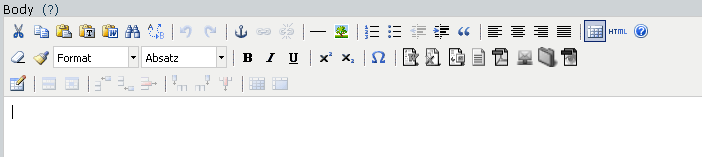
\includegraphics[width=\textwidth]{./images/tinymce-edit.png}
	\caption{Ansicht des TinyMCE WYSIWYG Editors}
	\label{fig:tinymceedit}
\end{figure}

\subsection{Einf�gen eines Bildes (mit TinyMCE)}
\label{insimage}

Wurde ein Bild wie unter Punkt \ref{upload} beschrieben im \ximsterm{Container} erstellt bzw. ist es bereits an
anderer Stelle ins \otherterm{XIMS} hochgeladen worden, ist das Einf�gen in das Dokument ein
Leichtes. Im Folgenden werden die grundlegenden Schritte beschrieben:

\begin{enumerate}
	\item {Der Cursor muss sich an der Stelle befinden, an der das Bild eingef�gt
werden soll.}
	\item {Durch Klicken auf das �Bild einf�gen/ver�ndern-Icon� �ffnet sich der Ei"-gen"-schaf"-ten-Dia"-log. �ber
diesen Dialog kann dem Bild eine Beschreibung und ein Titel gegeben werden (Abbildung \ref{fig:tinymceimageprop1}) sowie die Ausrichtung,  Breite, H�he, Randbreite, horizontaler und vertikaler Abstand (Abbildung \ref{fig:tinymceimageprop2}) f�r jedes Bild angegeben werden.}

%\begin{figure}[!ht]
%	\centering
%		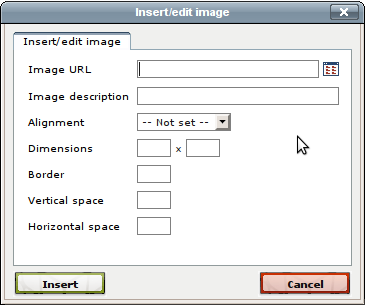
\includegraphics[width=0.55\textwidth]{./images/tinymce-imagepopup-solo.png}
%	\caption{Eigenschaften von Bildern in
%Dokumenten ver�ndern}
%	\label{fig:tinymceimageprop}
%\end{figure}

\begin{figure}[!ht]
	\centering
		\includegraphics[width=0.75\textwidth]{./images/tinymce-image-adv-1.png}
	\caption{Eigenschaften von Bildern in
Dokumenten ver�ndern}
	\label{fig:tinymceimageprop1}
\end{figure}

\begin{figure}[!ht]
	\centering
		\includegraphics[width=0.75\textwidth]{./images/tinymce-image-adv-2.png}
	\caption{Erweiterte Eigenschaften von Bildern}
	\label{fig:tinymceimageprop2}
\end{figure}

	\item {Durch Klicken auf das �Durchsuchen-Icon� �ffnet sich der Durchsuchen-Dialog. An
dieser Stelle k�nnen Sie den Pfad zum Bild bzw. dessen Titel
eingeben. Alternativ besteht die M�glichkeit im \otherterm{XIMS}-Verzeichnisbaum
nach dem gew�nschten Bild zu suchen. Mit Bet�tigen des �Store
Back�-Buttons wird das Bild an der Cursor-Position eingef�gt.}
\end{enumerate}

\begin{figure}[!ht]
	\centering
		\includegraphics[width=0.9\textwidth]{./images/suchebild.png}
	\caption{Auswahldialog zum Einf�gen eines Bildes}
	\label{fig:searchimage}
\end{figure}

\begin{Hinweis}
  Vermeiden Sie Bilder mit einer gr��eren Breite als 600 Pixel, weil
  dadurch das UIBK-Design beeintr�chtigt wird.
\end{Hinweis}

\subsection{Einf�gen eines Hyperlinks}
\label{inslink}

\paragraph{Automatische Hyperlinkerzeugung}
Wird in den WYSIWYG Editoren eine \nolinkurl{http://}-Adresse im Flie�text eingegeben,
wird diese vom Editor automatisch als \otherterm{URL} erkannt und in weiterer Folge als
Hyperlink erstellt.

\paragraph{Hyperlink unter Anleitung erstellen (\otherterm{TinyMCE})}

\begin{enumerate}
\item {Der Text der zum Hyperlink werden soll muss markiert sein.}
\item {Durch Klicken des �Link einf�gen/ver�ndern-Icons� �ffnet sich
    der Dialog zum Erstellen/Editieren eines Hyperlinks.}

  \begin{figure}[!ht]
    \centering
    \includegraphics[width=0.5\textwidth]{./images/insertlink.png}
    \caption{Hyperlink \otherterm{Dialogfenster}}
    \label{fig:hyperlinkdialog}
  \end{figure}

\item {Ein Klick auf das �Durchsuchen-Icon� �ffnet den Durchsuchen-Dialog.}
  
  \begin{figure}[!ht]
    \centering
    \includegraphics[width=0.9\textwidth]{./images/browselink.png}
    \caption{Erstellen eines Hyperlinks mit Dialog}
    \label{fig:linkerstellendialog}
  \end{figure}

\item {Das Linkziel kann analog zur Auswahl eines Bildes erstellt werden. Im Feld �Enter a title� kann der gew�nschte Linktext, falls
    abweichend vom Linkziel, eingegeben werden.

    \begin{Hinweis}
      Es besteht nat�rlich nicht nur die M�glichkeit eine URL
      einzuf�gen, sondern es kann auch auf andere Objekte wie
      beispielsweise Dateien u.�. verlinkt werden.
    \end{Hinweis}

    Optional kann auch das Zielfenster (Target) des Hyperlinks angegeben
    werden. Von dieser M�glichkeit wird jedoch zu Gunsten der Barrierefreiheit
    abgeraten. Es wird empfohlen dieses Feld leer zu lassen.}
\item {Nach dem Best�tigen mit dem �Store Back�-Button erscheint der erstellte
    Hyperlink im Editor.}
\end{enumerate}

\paragraph{Interne Links in Dokumenten (\otherterm{TinyMCE})}

\begin{figure}[!ht]
	\centering
		\includegraphics[width=0.4\textwidth]{./images/tinycontextimage.png}
	\caption{TinyMCE: Im Kontext-Men� k�nnen Links
eingef�gt/"-ver�ndert/"-entfernt werden.}
	\label{fig:tinycontextimage}
\end{figure}

Um auf einzelne Abschnitte innerhalb eines Dokuments verlinken zu k�nnen,
m�ssen zuerst Lesezeichen (�Anchors�) definiert werden, auf die sp�ter verwiesen
werden kann. Um ein solches Lesezeichen zu setzen, markieren Sie den
gew�nschten Text, zu welchem sp�ter verwiesen werden soll und klicken dann auf
das Lesezeichen Symbol. Sp�ter k�nnen Sie beim Erstellen von Hyperlinks das
Linkziel als \texttt{\#Name-des-Ankers} angeben.

\begin{figure}[!ht]
	\centering
		\includegraphics[width=0.5\textwidth]{./images/tinylinkanchor.png}
	\caption{TincMCE: Auf zuvor gesetzte Lesezeichen kann
sp�ter verwiesen werden.}
	\label{fig:tinyankerdialog}
\end{figure}

Im Feld �Adresse� kann nun auf das soeben erstelle Lesezeichen Bezug genommen
werden, in diesem Fall z.\,B. mit \texttt{seitenende} (siehe Abb.~\ref{fig:tinyankerdialog}).

\subsection{Importieren von MS-Word-Text in \otherterm{TinyMCE}}
\label{importword}

Der WYSIWYG-Editor \otherterm{TinyMCE} ist in der Lage, Texte aus MS-Word zu importieren
und dabei die Formatierungen weitgehend beizubehalten. Hierf�r sind folgende
Schritte notwendig.

\begin{enumerate}
	\item {Der markierte Text bzw. Textausschnitt in MS-Word wird mit Klick auf das
�Kopieren-Icon� bzw. mit dem Tastaturk�rzel �Strg + C� kopiert.}
	\item {Im WYSIWYG-Editor \otherterm{TinyMCE} kann der zuvor kopierte MS-Word-Text �ber
das �Einf�gen-Icon� bzw. mit �Strg + V� eingef�gt werden. (Weiters
besteht die M�glichkeit, den Text unformatiert oder als Text formatiert
einzuf�gen.)}
\end{enumerate}

\subsection{Zus�tzliche Funktionen (\otherterm{TinyMCE})}
\label{tinyfeatures}

Der Editor TinyMCE beinhaltet noch eine Reihe weiterer zus�tzlicher Funktionen wie
zum Beispiel das Wechseln zwischen WYSIWYG- und HTML-Ansicht, das Einf�gen
von Tabellen bzw. von diversen Sonderzeichen.


\clearpage

\section{Inhalte �ffentlich zug�nglich machen}
\label{inhaltepublizieren}

In \otherterm{XIMS} erstellte Objekte bzw. ver�nderte Versionen von bereits publizierten
Objekten sind nicht automatisch f�r die �ffentlichkeit sichtbar. Objekte m�ssen
explizit ver�ffentlicht werden!
Das Zusammenspiel zwischen Content Management und Pr�sentation f�r die
�ffentlichkeit zeigt die folgende Darstellung \ref{fig:xims-zusammenspiel}.

\begin{figure}[!ht]
	\centering
		\includegraphics[width=\textwidth]{./images/xims-zusammenspiel.png}
	\caption{\otherterm{XIMS} Zusammenspiel
Inhalteverwaltung und Pr�sentation}
	\label{fig:xims-zusammenspiel}
\end{figure}

Das Objekt (Dokument, Ordner, Datei, Bild, etc.), welches in \otherterm{XIMS} erstellt worden
ist, existiert vorerst nur in der \otherterm{XIMS}-Datenbank (1). Erst wenn das Objekt
ver�ffentlicht wird (�ver�ffentlichen� bzw. �publish�) (2), wird dieses in Form
einer XML-Datei in das Dateisystem des Webservers kopiert (3) und ist von diesem
Zeitpunkt an �ffentlich sichtbar.
An der Uni Innsbruck ist \otherterm{XIMS} bzw. AxKit so konfiguriert, dass der \ximsterm{SiteRoot} \path{/uniweb}
�ffentlich unter der Adresse \url{http://www.uibk.ac.at/} zu erreichen ist. Insofern spiegeln
die Pfade der \otherterm{XIMS} \ximsterm{Container} unter \path{/uniweb} die URLs unter
\url{http://www.uibk.ac.at/} wieder, d.h. Objekte in \otherterm{XIMS} unter dem Pfad
\path{/uniweb/fakultaeten/xxx} sind �ffentlich (wenn �ber \otherterm{XIMS} ver�ffentlicht) unter
\nolinkurl{http://www.uibk.ac.at/fakultaeten/xxx} verf�gbar.

\subsection{Objekte ver�ffentlichen (Publish)}
\label{publizieren}

Objekte k�nnen durch das Klicken auf das �Publizieren-Icon� ver�ffentlicht werden. Beim
erstmaligen \otherterm{Publizieren} eines erstellten Objekts erscheint folgendes \otherterm{Dialogfenster},
das ein �Ver�ffentlichen� oder ein �Abbrechen� zur Auswahl stellt.

\begin{figure}[!ht]
	\centering
		\includegraphics[width=0.9\textwidth]{./images/XI5S-publish.png}
	\caption{Dialog zum Ver�ffentlichen von Objekten}
	\label{fig:xims-publish}
\end{figure}

Bricht man den Publikationsvorgang ab (Abbrechen), ist das Objekt weiterhin nur in
der \otherterm{XIMS}-Datenbank pr�sent und nicht �ffentlich zug�nglich.
Nach dem Klicken des �Ver�ffentlichen�-Buttons erscheint eine Erfolgsmeldung,
die best�tigt, dass das Objekt erfolgreich ver�ffentlicht wurde, als XML-Datei im
Dateisystem vorliegt und somit �ffentlich erreichbar ist.

\subsection{Wiederver�ffentlichen (Republish)}
\label{republish}

Wurden bei einem vormals ver�ffentlichten Objekt �nderungen vorgenommen (siehe
Punkt \ref{icons}), m�ssen dessen Inhalte nochmals ver�ffentlicht
(�Wiederver�ffentlichen� oder �Republish�) werden. Get�tigte �nderungen (vor
dem Wiederver�ffentlichen) werden in dem Fall wiederum nur in der \otherterm{XIMS}-Datenbank
gespeichert, sind jedoch noch nicht im Dateisystem aktualisiert.

\begin{figure}[!ht]
	\centering
		\includegraphics[width=0.9\textwidth]{./images/XI5S-republish.png}
	\caption{Dialog zum erneuten Ver�ffentlichen von Objekten}
	\label{fig:xims-republish}
\end{figure}

Bricht man den Publikationsvorgang ab (�Abbrechen�), ist das Objekt weiterhin in
nicht aktualisierter Form ver�ffentlicht.
�Ver�ffentlichen r�ckg�ngig machen� (Unpublish) macht eine vormalige
Ver�ffentlichung r�ckg�ngig und l�scht die �ffentlich zug�ngliche Version des
Objekts im Dateisystem und das Objekt ist ab diesem Zeitpunkt nur mehr in der
\otherterm{XIMS}-Datenbank gespeichert.
�Wiederver�ffentlichen� (Republish) aktualisiert die Version des Objekts im
Dateisystem des Webservers. Somit sind die Versionen in der Datenbank und im Dateisystem des Webservers identisch (siehe Abb.~\ref{fig:xims-zusammenspiel}).

\subsection{L�schen und Verschieben ver�ffentlichter Objekte}
\label{deletepublished}

In bestimmten F�llen ist es gew�nscht, ver�ffentlichte Objekte nicht mehr �ffentlich
zur Verf�gung zu stellen. Ein Szenario ist beispielsweise, dass eine PDF-Datei,
welche zum Download angeboten wurde, nicht mehr �ffentlich zur Verf�gung
stehen soll. Das entsprechende Objekt muss daher aus dem Dateisystem des
Webservers gel�scht werden. Das geschieht mit Hilfe der Funktion
�Ver�ffentlichen r�ckg�ngig machen� (Unpublish). Ein L�schen der Datei im
\otherterm{XIMS} ist per se nicht notwendig.

Um Inkonsistenzen der \otherterm{XIMS}-Objekte zu vermeiden, ist das System mit einem
�Sicherungsmechanismus� ausgestattet:
Nachdem Objekte ver�ffentlicht wurden, verhindert \otherterm{XIMS} das Verschieben bzw.
L�schen ebensolcher, selbst wenn man grunds�tzlich die notwendigen Rechte daf�r
hat (siehe Punkt \ref{gesperrteobjekte}).

\begin{figure}[!ht]
	\centering
		\includegraphics[width=\textwidth]{./images/publishednotpublished.png}
	\caption{Ver�ffentlichtes und unver�ffentlichtes Objekt in der \otherterm{XIMS}-Containeransicht}
	\label{fig:publishednotpublished}
\end{figure}

Um nun ein ver�ffentlichtes Objekt verschieben bzw. l�schen zu k�nnen, muss die
Ver�ffentlichung dieses Objekts zuerst r�ckg�ngig gemacht werden (siehe Punkt \ref{inhaltepublizieren}). Durch das Zur�cknehmen der Ver�ffentlichung ist das Objekt nur noch in der
\otherterm{XIMS}-Datenbank vorhanden. Es ist wieder m�glich, das Objekt zu verschieben (mit
Hilfe des �Verschieben-Icons�) bzw. zu l�schen (�L�schen-Icon�).

%
% Option ist derzeit in Xims deaktiviert, das Sie nicht richtig funktioniert und eigentlich nicht gebraucht wird
%
%\subsection{Vorschau auf Objekte in ver�ffentlichtem Zustand}
%\label{preview}
%
%Die Darstellung von Dokumenten im \otherterm{XIMS} variiert teilweise von der Darstellung des
%Dokuments im ver�ffentlichten Zustand. Um als Redakteur eine Vorstellung zu
%bekommen, wie ein Dokument im ver�ffentlichten Zustand aussehen wird, bietet
%\otherterm{XIMS} eine Ver�ffentlichungsvorschau an.
%
%\begin{figure}[!ht]
%	\centering
%		\includegraphics[width=\textwidth]{./images/veroeffentlichungsvorschau.png}
%	\caption{Ver�ffentlichungsvorschau}
%	\label{fig:veroeffentlichungsvorschau}
%\end{figure}
%
%Der Link �Ver�ffentlichungsvorschau� (Publishing Preview) �ffnet ein neues
%Fenster in dem der Inhalt des Dokuments integriert in das UIBK-Design dargestellt
%wird. Dies entspricht der Darstellung des Dokuments, wie es die Benutzer (nach dem
%eigentlichen Ver�ffentlichungsvorgang) �ffentlich pr�sentiert bekommen.
%
%\begin{figure}[!ht]
%	\centering
%		\includegraphics[width=\textwidth]{./images/veroeffentlichungsvorschau-live.png}
%	\caption{Ver�ffentlichungsvorschau: Zeigt das Dokument im eigentlichen Design ohne
%zu ver�ffentlichen}
%	\label{fig:veroeffentlichungsvorschau-live}
%\end{figure}
%
%\begin{Hinweis}
%  Objekte, die in der Ver�ffentlichungsvorschau betrachtet werden,
%  zeigen in der Darstellung bereits alle Ver�nderungen. Dabei ist zu
%  beachten, dass die Ver�ffentlichungsvorschau das Objekt nicht
%  ver�ffentlicht. Da es sich um eine reine Vorschau handelt, existiert
%  das Objekt in der ver�nderten Version weiterhin nur in der
%  \otherterm{XIMS}-Datenbank. Um die Ver�nderungen f�r die
%  �ffentlichkeit sichtbar zu machen, m�ssen Objekte ver�ffentlicht
%  bzw. wiederver�ffentlicht werden.
%\end{Hinweis}

\clearpage

\section{Berechtigungsmechanismus in \otherterm{XIMS}}
\label{berechtigungen}

\otherterm{XIMS} verf�gt �ber ein umfangreiches Berechtigungssystem. Dieses erm�glicht eine
sehr feingranulare Steuerung von Berechtigungen. Berechtigungen k�nnen auf
Basis einzelner Benutzer bzw. Rollen (z.\,B. zur Verwaltung von Benutzergruppen)
vergeben werden. Berechtigungen regeln die Privilegien auf \otherterm{XIMS}-Objekte.

Ein Benutzer kann beispielsweise die Berechtigung besitzen, bestimmte Dokumente
zu lesen, ein anderer Benutzer hingegen kann Objekte editieren bzw. aus dem
System l�schen.

F�r jedes einzelne in \otherterm{XIMS} verwaltete Objekt sind eigene Zugriffsrechte in einer
sogenannten ">Access-Control-List"< (ACL) gespeichert. Mit einem Klick auf das �Zugriffskontrolle/Rechteverwaltung-Icon�
des gew�nschten Objekts k�nnen bestehende Berechtigungen von Benutzern bzw.
Rollen gesichtet bzw. ver�ndert werden. Hat ein Benutzer das �GRANT�-Recht
(Verwaltungsrecht), so darf dieser Benutzer auch bestehende Berechtigungen
ver�ndern bzw. neue hinzuf�gen.

\begin{Hinweis}
  Die Berechtigungen werden f�r das jeweilige, einzelne Objekt
  durchgesetzt; jemanden blo� aus einem �bergeordneten Verzeichnis
  auszusperren ist also nicht ausreichend: Die darunter liegenden
  Objekte k�nnten trotzdem (z.\,B. �ber die Suche) direkt angesprungen
  werden, wenn ihre eigene ACL dies zul�sst!
\end{Hinweis}

\subsection{Rechte-�bersicht}
F�hrt man mit der Maus �ber das Icon zum Rechteverwalten (Schl�sselsymbol) eines Objekts, �ffnet sich ein sogenannter Tooltip, der eine �bersicht �ber die derzeit vergebenen Rechte gibt. Gesetzte Rechte in der �bersicht, erkennen Sie an der fetten Schrift und dem wei�en Hintergrund des Buttons. Nicht vergebene Rechte sind durchgestrichen und hellgrau unterlegt.

XIMS kennt die folgenden Privilegien:

\subsubsection{Standardrechte (Basic Privileges)}
\label{standardrechte}
Standardrechte sind grundlegende Privilegien, die \otherterm{XIMS} zur Beschr�nkung des
Zugriffs auf Objekte zu vergeben hat. Sie sind �hnlich Dateisystemrechten auf
Betriebssystemebene (vgl. Windows/Unix-Zugriffsrechte auf Dateien bzw.
Verzeichnisse)

\paragraph{View (Lesen)}
Leserecht f�r Benutzer/Rolle.

\paragraph{Write (Schreiben)}
Schreibrechte f�r Benutzer/Rolle f�r ein Objekt. Dadurch k�nnen beispielsweise der
Titel bzw. Inhalt ver�ndert und geschrieben werden.

\paragraph{Create (Erstellen)}
Benutzer/Rolle darf ein neues Objekt in einem \ximsterm{Container} erstellen.

\paragraph{Delete (L�schen)}
Benutzer/Rolle darf ein Objekt l�schen.

\paragraph{Move (Verschieben)}
Benutzer/Rolle darf ein Objekt verschieben.

\subsubsection{Ver�ffentlichungsrechte (Publishing Privileges)}
\label{pubrechte}
\paragraph{Publish (Ver�ffentlichen)} Ein Benutzer bzw. eine Rolle hat das Recht Ver�ffentlichungsfunktionen
(�ver�ffentlichen�, �wiederver�ffentlichen�, �ver�ffentlichen
r�ckg�ngig machen�; siehe Punkt \ref{publizieren}) auszuf�hren.

\subsubsection{Verwaltungsrechte (Grant Privileges)}
\label{verwrechte}

\paragraph{Grant (Rechte gew�hren)} Besitzen Benutzer bzw. Rollen das Verwaltungsrecht (Grant Privilege), sind diese in
der Lage anderen Benutzern bzw. Rollen explizite Privilegien f�r Objekte
einzur�umen, d.h. Benutzer bzw. Rollen mit Verwaltungsrecht k�nnen Privilegien an
andere Benutzer bzw. Rollen vergeben.


\subsection{Berechtigungen vergeben und verwalten}
%\subsection{Berechtigungen eines Benutzers bzw. einer Rolle}
\label{berechtigungen-benutzer}
Um bestehende Berechtigungen zu �ndern oder neue Berechtigungen zu vergeben, klicken Sie auf das Icon zur ">Rechteverwaltung"<. Es erscheint eine Dialog-Seite (siehe Abbildung \ref{fig:manage-acl}) auf der Sie im oberen Teil (1) neue Rechte vergeben k�nnen. Im zweiten Abschnitt (2) sehen Sie eine Tabelle mit den derzeit vergebenen Rechten und der M�glichkeit, diese Berechtigungen zu �ndern oder zu entfernen.

\begin{figure}[!ht]
	\centering
		\includegraphics[width=\textwidth]{./images/manage-acl2.png}
	\caption{Rechte verwalten}
	\label{fig:manage-acl}
\end{figure}

\paragraph{Neue Berechtigungen vergeben}
%Geben Sie den Namen der Rolle oder des Benutzers, an den Sie Privilegien vergeben wollen, in das entsprechende Feld ein\footnote{Sie k�nnen gleiche Privilegien gleichzeitig an mehrere Nutzer vergeben indem Sie die Namen der Benutzer und Rollen durch Komma getrennt in das Feld eingeben}. M�chten Sie die Berechtigungen gleichzeitig nicht nur an das gew�hlte Objekt sondern auch an alle Kindobjekte (z.B. bei einem Ordner auch an alle enthaltenen Objekte und Unterorder) vergeben, aktivieren Sie die Option ">Rechte rekursiv vergeben/entziehen"<. Anschlie�end dr�cken Sie den ">Speichern"<-Button. Nach dem gleichen Schema k�nnen Sie einem oder mehreren Nutzern auch Rechte entziehen. Dazu klicken Sie statt ">Speichern"< den ">Rechte entfernen"<-Button.
Geben Sie den Namen der Rolle oder des Benutzers, an den Sie Privilegien vergeben wollen, in das entsprechende Feld ein\footnote{Sie k�nnen gleiche Privilegien gleichzeitig an mehrere Nutzer vergeben indem Sie die Namen der Benutzer und Rollen durch Komma getrennt in das Feld eingeben}. Anschlie�end dr�cken Sie den ">Speichern"<-Button. Nach dem gleichen Schema k�nnen Sie einem oder mehreren Nutzern auch Rechte entziehen. Dazu klicken Sie statt ">Speichern"< den ">Rechte entfernen"<-Button.

\paragraph{Bestehende Berechtigungen verwalten}

%\begin{figure}[!ht]
%	\centering
%		\includegraphics[width=\textwidth]{./images/bestehendeberechtigungen.png}
%	\caption{Bestehende Berechtigungen verwalten}
%	\label{fig:permissions}
%\end{figure}

Um bestehende Berechtigungen eines Benutzers zu ver�ndern, gehen Sie in der Tabelle mit den vergebenen Rechten in die Zeile des Benutzers bzw. der Rolle, deren Berechtigungen Sie �ndern wollen. Dort aktivieren bzw. deaktivieren Sie das Privileg durch Klick auf den entsprechenden Button in der Rechte�bersicht und dr�cken anschlie�end ">Speichern"<. Wollen Sie einem Benutzer oder einer Rolle alle Rechte entziehen, klicken Sie auf den ">Rechte entfernen"<-Button in der Zeile des Benutzers/ der Rolle.

Um den Dialog zum Rechte verwalten zu verlassen ohne Privilegien zu �ndern, w�hlen Sie ">Abbrechen"<.

%folgt man dem Link �Rechte verwalten� (Manage Privileges). Daraufhin folgt ein Dialog
%mit zwei unterschiedlichen Bereichen (siehe Abb.~\ref{fig:permissionadmin}). Der obere Bereich (1) dient
%zur Steuerung der Berechtigungen f�r den entsprechenden Benutzer bzw. der
%entsprechenden Rolle. Rollen sind i.d.R mit dem UIBK-Pr�fix gekennzeichnet. Im
%unteren Bereich (2) k�nnen die zuvor explizit dem Benutzer bzw. der Rolle
%zugewiesenen Berechtigungen wieder entfernt werden. D.h. �ber den �Rechte entfernen�-Button wird der Benutzer bzw. die
%Rolle aus der Berechtigungstabelle (siehe Abb.~\ref{fig:permissions}) des Objektes vollkommen
%entfernt und verliert alle damit verbundenen Berechtigungen.
%
%\begin{figure}[!ht]
%	\centering
%		\includegraphics[width=\textwidth]{./images/benutzerrechteverwalten.png}
%	\caption{Verwalten von Benutzer- bzw. Rollenprivilegien}
%	\label{fig:permissionadmin}
%\end{figure}
%
%Der obere Bereich (1) untergliedert sich in drei unterschiedliche Arten von
%Privilegien: Standardrechte, Ver�ffentlichungsrechte und Verwaltungsrechte
%(siehe auch Punkt \ref{zugriffsrechte}).
%Standardrechte sind �bliche Berechtigungen, wie das Recht zu lesen bzw. zu
%schreiben. Das Ver�ffentlichungsrecht erm�chtigt einen Benutzer bzw. eine Rolle,
%das Objekt zu ver�ffentlichen. Das Verwaltungsrecht gew�hrt einem Benutzer bzw.
%einer Rolle das Recht, anderen Personen Privilegien f�r ein Objekt einzur�umen
%bzw. wegzunehmen.
%Die Ver�nderungen der Privilegien werden erst durch das Dr�cken des
%�Speichern�-Buttons wirksam.
%Im unteren Bereich (2) k�nnen einem Benutzer bzw. der Rolle s�mtliche Rechte auf
%das Objekt genommen werden. D.h. durch das Dr�cken des �Rechte entfernen�-
%Buttons (Revoke Grants) wird der Benutzer bzw. die Rolle aus der �Access Control
%List� (ACL) entfernt und scheint somit nicht mehr in der Liste der Benutzer auf,
%welche explizite Rechte auf das Objekt zugewiesen bekommen haben.

\begin{Hinweis}
  Wenn Sie einer Rolle, z.\,B.: UIBK:ALL, alle Rechte nehmen wollen,
  l�schen Sie bitte die Rolle mit �Rechte entfernen� komplett aus der
  ACL. Wenn Sie die Rolle belassen und stattdessen alle Privilegien
  entfernen, sperren Sie damit alle Rollenmitglieder aus -- im Falle
  von UIBK:ALL vermutlich auch sich selbst!
\end{Hinweis}

%Um Benutzern bzw. Rollen, die bisher noch keine expliziten Rechte f�r ein Objekt
%haben, Privilegien zu erteilen, muss der Benutzer bzw. die Rolle zuerst ausfindig
%gemacht werden. Zu diesem Zweck bietet \otherterm{XIMS} in der Berechtigungsvergabe die
%M�glichkeit nach Benutzern bzw. Rollen zu suchen.
%
%\begin{figure}[!ht]
%	\centering
%		\includegraphics[width=\textwidth]{./images/benutzersuchen.png}
%	\caption{Benutzer bzw. Rollen ausfindig machen}
%	\label{fig:benutzersuchen}
%\end{figure}

%\textbf{Suche nach Benutzern:}
%
%Um nach einzelnen Benutzern zu suchen, ist die Benutzerkennung in das
%Eingabefeld einzugeben (z.\,B. C102XX). Mit einem anschlie�enden Klick auf den
%�Suchen�-Button, sucht \otherterm{XIMS} nach dem besagten Benutzer und listet diesen auf. In
%weiterer Folge k�nnen dem Benutzer �ber den Link �Neue Rechte vergeben�
%gew�nschte Privilegien einger�umt werden.
%
%\textbf{Suche nach Rollen:}
%
%Um nach bestehenden Rollen zu suchen, gibt man den Namen der Rolle (i.d.R.
%beginnend mit �UIBK:�) in das Suchfeld ein (beispielsweise UIBK:ZID) und w�hlt im
%Auswahlfeld �Rolle� (anstatt �BenutzerInnen�) aus. Nach einem anschlie�enden
%Klick auf �Suchen� listet \otherterm{XIMS} alle Rollen auf, die den Suchbegriff im Namen
%enthalten. Gew�nschte Privilegien auf gefundene Rollen k�nnen analog zur Vergabe
%von Privilegien f�r Benutzer vergeben werden.

\subsection{Rollenverwaltung}
\label{rollenverwaltung}
Tritt ein Mitarbeiter neu in eine Organisationseingheit ein bzw. verl�sst sie, ist es oft n�tig ihm auf alle Objekte in einem bestimmten Bereich Privilegien zu geben bzw. diese zu entfernen. Hier ist die Arbeit mit Rollen ein praktisch Mittel. Anstatt jedem einzelnen Mitarbeiter Rechte einzeln zuzuweisen, vergibt man stattdessen die gew�nschten Rechte an eine Rolle und f�gt alle Benutzer, die die selben Rechte auf ein Objekt oder einen ganzen Bereich erhalten sollen dieser Rolle hinzu. Um Benutzer zu einer Rolle hinzuf�gen oder zu entfernen kann die Rollenverwaltung verwendet werden. Der jeweilige Rollenadministrator kann sich mit seiner
Benutzerkennung (z.\,B. C102XX) unter \url{http://xims.uibk.ac.at/roles} einloggen.

\begin{figure}[!ht]
	\centering
		\includegraphics[width=\textwidth]{./images/rollenverwaltung.png}
	\caption{Login Rollenverwaltung}
	\label{fig:rollenverwaltung}
\end{figure}

\begin{Hinweis}
Es wird empfohlen so wenig Rechte wie m�glich an einzelne Benutzer zu vergeben. Die Arbeit mit Rollen dient im Endeffekt nicht nur der �bersichtlichkeit bei den vergebenen Rechten sondern vor allem auch der Vereinfachung der Wartung der Privilegien eines Bereichs.
\end{Hinweis}


\clearpage

\section{Spezielle Funktionen}
\label{specfeatures}

F�r den Fall dass der XIMS-Standardfunktionsumfang nicht ausreicht, bietet XIMS eine Reihe 
weiterer Funktionen an, die dem fortgeschrittenen Benutzer zus�tzlichen Anpassungsfreiraum einr�umen.

\subsection{Links zum Dokument (Document Links)}
\label{doclinks}

Bei den so genannten �Links zum Dokument� handelt es sich um weiterf�hrende
Links zum Thema eines Dokuments. Links zum Dokument werden am Ende des
Inhaltsbereichs dargestellt.

\begin{figure}[!ht]
	\centering
		\includegraphics[width=\textwidth]{./images/linkszumdokument.png}
	\caption{Links zum Dokument werden am Ende des Inhaltsbereichs dargestellt}
	\label{fig:dokumentlinks-live}
\end{figure}

\paragraph{Links zum Dokument erstellen}

�Links zum Dokument� lassen sich -- wie der Name bereits vermuten l�sst -- speziell
zu einem Dokument erstellen. Um einen �Link zum Dokument� zu erstellen, muss
zuerst in die Vollansicht des gew�nschten Dokuments gewechselt werden.

\begin{figure}[!ht]
	\centering
		\includegraphics[width=\textwidth]{./images/create-linkzumdokument.png}
	\caption{Links zum Dokument werden �ber die Vollansicht des Dokuments erstellt}
	\label{fig:dokumentlinks}
\end{figure}

Zu beachten ist, dass �Links zum Dokument� nur erstellt werden k�nnen, wenn der
aktuelle Benutzer �ber das �Create�-Recht f�r das entsprechende Dokument verf�gt.
�Links zum Dokument� k�nnen einerseits auf andere in \otherterm{XIMS} erzeugte Objekte
(interne Links) und andererseits auf externe Webseiten (au�erhalb der Dom�ne
\url{http://www.uibk.ac.at}) verweisen.

%\begin{figure}[!ht]
%	\centering
%		\includegraphics[width=\textwidth]{./images/create-linkzumdokument2.png}
%	\caption{Dialog zum Erstellen von �Links zum Dokument�}
%	\label{fig:dokumentlinks2}
%\end{figure}

\subparagraph{Interne Links}

F�r interne Links muss der Zielpfad im Eingabefeld \ximsterm{Location} 
relativ zum Dokument
eingegeben werden. D.h. f�r einen Verweis auf ein Dokument mit 
%der \ximsterm{Location}
dem Pfad 
\nolinkurl{hallo.html} (welches sich im selben \ximsterm{Container} wie das Dokument zu dem der Link
erstellt wird befindet) ist als 
\ximsterm{Location} 
f�r den �Link zum Dokument� \nolinkurl{hallo.html}
einzugeben.

\subparagraph{Externe Links}

F�r externe �Links zum Dokument� ist es zwingend erforderlich die vollst�ndige URI
im Eingabefeld �\ximsterm{Location}� mit vorangestelltem \nolinkurl{http://} einzugeben (z.\,B.:
\url{http://www.orf.at}).

Bez�glich einer Beschreibung der Eingabefelder �Titel�, �\otherterm{Schlagw�rter}�, �Zusammenfassung�, �Objekt als neu markieren� und �Zugriffsrechte erstellen� wird auf den Punkt \ref{urllinks} verwiesen.

\paragraph{Editieren von �Links zum Dokument�}

Ein Klick auf das �Bearbeiten-Icon� �ffnet die Editiermaske zum Ver�ndern eines
�Links zum Dokument�.

\begin{figure}[!ht]
	\centering
		\includegraphics[width=\textwidth]{./images/edit-linkzumdokument.png}
	\caption{Jeder �Link zum Dokument� kann �ber die gewohnten Icons bearbeitet werden}
	\label{fig:editdokumentlink}
\end{figure}

Weiters k�nnen f�r jeden �Link zum Dokument� verschiedenen Rechte
vergeben bzw. ver�ndert werden. Die L�schen-Funktion (rotes Kreuz)
erm�glicht das L�schen von �Links zum Dokument�.

\subsection{\ximsterm{DepartmentRoot} Navigation}
\label{depnav}

Usability-Studien haben gezeigt, dass Benutzer die Navigation auf
Webseiten am oberen bzw. im linken Bereich des Browser-Fensters
suchen. Aus diesem Grund ist die grundlegende Navigation des
UIBK-Designs auch auf diese Erkenntnis ausgerichtet. Neue Besucher auf
DepartmentRoot Seiten werden die \ximsterm{DepartmentLinks} zur
Hauptnavigation rasch finden. Die \ximstermdef{DepartmentSpeziallinks}
sind im Gegensatz dazu auf h�ufig wiederkehrende Besucher ausgerichtet
und sollen zum schnelleren Auf"|finden relevanter bzw. h�ufig
ver�nderter Inhalte dienen.

\subsubsection{DepartmentLinks}
\label{deplinks}

\ximstermdef{DepartmentLinks} stellen die grunds�tzliche Navigation
der jeweiligen Organisationseinheit dar. Diese Navigation erm�glicht
es, durch die wichtigsten Bereiche bzw. Seiten navigieren zu k�nnen.
Zur Erstellung der \ximsterm{DepartmentLinks} sind im Wesentlichen
folgende Schritte notwendig:

\begin{itemize}
\item {Erstellen eines Verzeichnisses (Ordner) mit Pfad und Titel \path{departmentlinks}. Der Pfad und der Titel des Verzeichnisses m�ssen zwingend \path{departmentlinks} hei�en. Bitte achten Sie hier besonders auf m�gliche Tippfehler.}

\begin{figure}[!ht]
  \centering
  \includegraphics[width=\textwidth]{./images/create-departmentlinksfolder.png}
  \caption{Erstellen des Verzeichnisses \texttt{departmentlinks}}
  \label{fig:createdeplinkfolder}
\end{figure}
	
\item {Im n�chsten Schritt m�ssen im soeben erstellten Verzeichnis mit dem Pfad \path{departmentlinks} all jene  \ximsterm{URLLink}-Objekte erstellt werden, die als Navigation bzw. DepartementLinks zur Verf�gung stehen sollen\footnote{Die Anleitung zum Erstellen von \ximsterm{URLLink}-Objekten kann unter Punkt \ref{urllinks} nachgelesen werden.} 
Die \ximsterm{Location} der Links muss relativ zum \ximsterm{SiteRoot}\footnote{An der Uni Innsbruck hei�t der \ximsterm{SiteRoot} \path{uniweb}.} sein. Der Titel des \ximsterm{URLLink} erscheint dann als Titel des Men�-Punkts.
Um zum Beispiel einen Men�-Eintrag ">Aktuelles"< zu erstellen der auf ein Dokument mit dem Pfad \path{/uniweb/institut-xy/aktuelles.html} verweist, muss im muss im Eingabefeld \ximsterm{Location} des \ximsterm{URLLink}-Objektes \path{/institut-xy/aktuelles.html} eingegeben werden und im Eingabefeld Titel ">Aktuelles"<.
Soll auf ein Verzeichnis bzw. dessen Index-Datei verwiesen werden, muss am Ende der Location unbedingt ein Schr�gstrich eingetragen werden. Auf das Verzeichnis \path{/uniweb/institut-xy/mitarbeiter} verweisen Sie indem Sie in der Location des \ximsterm{URLLink} den Pfad \path{/institut-xy/mitarbeiter/} angeben. Klickt ein Besucher der Webseite auf den Men�-Eintrag ">Mitarbeiter"<, bekommt er die Index-Datei des Verzeichnisses \path{/uniweb/institut-xy/mitarbeiter} (z.B. \path{/uniweb/institut-xy/mitarbeiter/index.html}) angezeigt.}
%Um zum Beispiel einen Verweis auf das \otherterm{XIMS}-Objekt mit dem Pfad \path{/uniweb/service/c102} zu erstellen, muss im Eingabefeld \ximsterm{Location} des \ximsterm{URLLink}-Objektes \path{/service/c102/} eingegeben werden. F�r das \otherterm{XIMS}-Objekt \path{/uniweb/geschichte/personal/index.html} die \ximsterm{Location} \path{/geschichte/personal/}.}

\begin{Hinweis}
Nutzen Sie die Option ">Ziel suchen"< um die \ximsterm{Location} eines \ximsterm{URLLink} zu definieren. So vermeiden Sie Fehler.
\end{Hinweis}
	
\item {Der n�chste Schritt ist das Ver�ffentlichen des departmentlinks-Verzeichnisses mitsamt den darin erstellten Links. Die konkrete Vorgehensweise f�r die Ver�ffentlichung von Objekten wird unter Punkt \ref{inhaltepublizieren} beschrieben.}

\begin{Hinweis}
  Es gen�gt das Verzeichnis \path{departmentlinks} zu ver�ffentlichen.
  Die darin enthaltenen \ximsterm{URLLink}s werden mit entsprechender
  Option automatisch mit ver�ffentlicht.
\end{Hinweis}

\item {Danach muss im \ximsterm{DepartmentRoot}-\ximsterm{Container} ein \ximsterm{Portlet} mit dem Pfad \path{departmentlinks_portlet.ptlt} und dem Titel ">departmentlinks\_portlet"< erstellt werden. Diese Namenskonventionen sind unbedingt einzuhalten damit die Navigation korrekt angezeigt wird. Das zuvor erstellte Verzeichnis \path{departmentlinks} muss im Feld �Ziel� eingetragen werden. (z.B. bequem �ber �Ziel suchen�.) Au�erdem muss die Checkbox der Zusammenfassung angeklickt sein.}

%\begin{Hinweis}
%  Das \ximsterm{Portlet} (sowohl \ximsterm{Location} als auch der
%  Titel) muss unbedingt \path{departmentlinks_portlet} hei�en. Das
%  zuvor erstellte Verzeichnis \path{departmentlinks} muss im Feld
%  �Ziel� eingetragen werden. (z.\,B. bequem �ber �Ziel suchen�.)
%  Au�erdem muss die Checkbox der Zusammenfassung angeklickt sein.
%\end{Hinweis}

\begin{figure}[!ht]
  \centering
  \includegraphics[width=\textwidth]{./images/create-departmentlinksportlet.png}
  \caption{Erstellen des DepartmentLinks-Portlets:
    �departmentlinks\_portlet�}
  \label{fig:createdeplinkportlet}
\end{figure}

\item {Im n�chsten Schritt muss das erstellte Portlet ver�ffentlicht werden.}

\item {In weiterer Folge muss das �departmentlinks\_portlet� dem
    \ximsterm{DepartmentRoot} zugewiesen werden. Dazu muss das
    �Bearbeiten-Icon� des \ximsterm{DepartmentRoot}-Verzeichnisses
    angeklickt werden, um �nderungen am \ximsterm{DepartmentRoot}
    durchf�hren zu k�nnen. Weisen Sie das Portlet am Besten �ber den Dialog zu der sich nach einem Klick auf ">Suche"< �ffnet. Haben Sie ein Portlet ausgew�hlt, klicken Sie anschlie�en auf ">Portlet zuweisen"< und speichern das Departmentroot.}

\begin{figure}[!ht]
  \centering
  \includegraphics[width=\textwidth]{./images/zuweisendepartmentlinksportlet.png}
  \caption{Zuweisen des DepartmentLinks \ximsterm{Portlet} zum
    DepartementRoot}
  \label{fig:deplinkportletzuweisen}
\end{figure}

\item {Der letzte Schritt ist das (Re)\otherterm{Publizieren} des
    editierten \ximsterm{DepartmentRoot} Ordners.}
\end{itemize} 

\subsubsection{\ximstermdef{SubDepartmentLinks} (Unternavigation)}
\label{subdeplinks}
 
Um eine Unternavigation zu erstellen, wird im Grunde mittels
\ximsterm{DepartmentLinks} auf \ximsterm{Container} verlinkt, die
wiederum DepartmentLinks enthalten. Auf diese Weise enth�lt das
eigentliche \ximsterm{DepartmentRoot} die Hauptnavigation (im Ordner
\path{departmentlinks}) und die darin enthaltenen
\ximsterm{DepartmentRoot}s -- auch Subdepartmentroots genannt --
enthalten ihrerseits jeweils die Unternavigation des jeweiligen
Punktes der Hauptnavigation.

\paragraph{Voraussetzungen}

Um eine Subnavigation erstellen zu k�nnen muss zuerst ein
\ximsterm{DepartmentRoot} (i.d.R. bereits vorhanden) und anschlie�end weitere darin enthaltene \ximsterm{DepartmentRoot}s erstellt
werden. Ebenso ist es m�glich eine bestehende Struktur in XIMS
entsprechend den ver�nderten Anforderungen anzupassen (es besteht die
M�glichkeit bestehende Ordner in \ximsterm{DepartmentRoot}s
umzuwandeln).

\begin{Hinweis}
  Der Benutzer muss entsprechende Berechtigungen zum Erstellen von
  \ximsterm{DepartmentRoot}s haben. Wenden Sie sich ggf. bitte an
  \href{mailto:XIMS-Support@uibk.ac.at}{\nolinkurl{XIMS-Support@uibk.ac.at}}.
\end{Hinweis}

\paragraph{Vorgehensweise}

Abbildung~\ref{fig:subdeplinks} zeigt die Hauptnavigation und die
Unternavigation bei aktivem Hauptnavigationseintrag. Es wird immer nur
die Unternavigation des aktuellen Hauptnavigationseintrages
dargestellt.

\begin{figure}[!ht]
  \centering
  \includegraphics[scale=0.7]{./images/subdeplinks.png}
  \caption{Beispiel: Hauptnavigation und Unternavigation}
  \label{fig:subdeplinks}
\end{figure}

Wie in Punkt \ref{deplinks} beschrieben befindet sich im Ordner
\path{departmentlinks} die Hauptnavigation, analog dazu ist in den
jeweiligen Ordnern mit Unternavigation ein Ordner
\path{subdepartmentlinks} enthalten. Der Ordner (welcher zwingend den Titel ">supdepartmentlinks"< und den
Pfad \path{subdepartmentlinks.ptlt} haben muss) enth�lt somit die
Unternavigationspunkte f�r den Hauptnavigationseintrag des
\ximsterm{DepartmentRoot}s.

\begin{compactitem}
\item{Erstellen des \ximsterm{DepartmentRoot}s, welches die
    Hauptnavigation (\ximsterm{DepartmentLinks}) enthalten wird.
    Dieses \ximsterm{DepartmentRoot} besteht in den allermeisten
    F�llen bereits.}
\item{Erstellen des \ximsterm{DepartmentRoot}s, welches die
    Unternavigation (\ximsterm{SubDepartmentLinks}) enthalten wird.
    Zum Beispiel \path{mitarbeiter}, \path{forschung} oder
    \path{links}.}
\item{Erstellen des Ordners \path{departmentlinks} im
    \ximsterm{DepartmentRoot} der Hauptnavigation. Dieser Ordner
    existiert in den meisten F�llen bereits (Wenn Sie schon eine
    Hauptnavigation haben ist eine �nderung nicht erforderlich!)}
\item{Erstellen des Ordners \path{subdepartmentlinks} in den
    \ximsterm{DepartmentRoot}s der Unternavigation.}
\item{Erstellen der \ximsterm{URLLink} Objekte im
    \path{departmentlinks} Ordner der Hauptnavigation. Die
    \ximsterm{URLLink}s m�ssen auf die soeben erstellten
    \ximsterm{DepartmentRoot}s der Unternavigation verweisen.}
\item{Erstellen eines Portlets mit Location
    \path{departmentlinks_portlet} im \ximsterm{DepartmentRoot} der
    Hauptnavigation. Dieses Portlet muss auf den Ordner
    \path{departmentlinks} zeigen und existiert in den meisten F�llen
    bereits.}
\item{Erstellen der \ximsterm{URLLink}-Objekte in den jeweiligen
    \path{subdepartmentlinks} Ordnern. Diese \ximsterm{URLLink}
    Objekte m�ssen auf jene Dokumente zielen, die durch einen Klick
    auf den jeweiligen Unternavigationspunkt angezeigt werden sollen.}
\item{Erstellen eines Portlets mit dem Titel ">subdepartmentlinks\_portlet"< und dem Pfad
    \path{subdepartmentlinks_portlet.ptlt} im \ximsterm{DepartmentRoot} der
    Unternavigation. Dieses Portlet muss auf den Ordner
    \path{subdepartmentlinks} der jeweiligen Unternavigation zeigen.}
\item{Zuweisen der Portlets zu den entsprechenden
    \ximsterm{DepartmentRoot}s.}
\item{Erstellen eines Dokumentes \nolinkurl{index.html} in den
    \ximsterm{DepartmentRoot}s der Unternavigation, welches beim Klick
    auf die Unternavigation als �bersichtsseite angezeigt wird.}
\item{(Wieder)ver�ffentlichen der neu erstellten bzw. ver�nderten Objekte.}
\end{compactitem}

\begin{Hinweis}
  Bei \ximsterm{URLLink} Objekten ist als Location immer der Pfad des
  Zielobjektes anzugeben. Bei \ximsterm{URLLink}s der Hauptnavigation
  muss ein Slash angeh�ngt werden, weil auf einen Ordner verwiesen
  wird, wodurch das jeweilige Index Dokument angezeigt wird und in
  weiterer Folge die Unternavigation aufklappt.
\end{Hinweis}

\subsubsection{DepartmentSpeziallinks}
\label{depspeclinks}

Das Erstellen der \ximsterm{DepartmentSpeziallinks} erfolgt analog zum Erstellen der
\ximsterm{DepartmentLinks}. Der Unterschied beschr�nkt sich auf die unterschiedliche
Bezeichnung des Pfads und Titels des DepartmentSpeziallinks-Verzeichnisses und des
zugeh�rigen \ximsterm{Portlet}s. Insofern wird auf Punkt \ref{deplinks} verwiesen. F�r die \ximsterm{DepartmentSpeziallinks} m�ssen der Titel und der Pfad des DepartmentSpeziallink-Verzeichnisses jeweils \path{speciallinks} lauten. Ebenfalls muss das DepartmentSpeziallink-\ximsterm{Portlet} den Titel ">speciallinks\_portlet"< und den Pfad \path{speciallinks_portlet.ptlt} besitzen und auf das Verzeichnis \path{speciallinks} (mit den gew�nschten Links als Inhalt) verweisen. Zuletzt ist das Portlet dem \ximsterm{DepartmentRoot} zuzuweisen.

\subsection{Department Images}
\label{depimg}

Das Einf�gen eines \ximstermdef{DepartmentImage}s hat das Ziel, die Individualit�t eines
Webauftritts einer Organisationseinheit zus�tzlich zu betonen und sich vom
Standard-Design ein wenig zu differenzieren.
Das \ximsterm{DepartmentImage} wird �hnlich wie die \ximsterm{DepartmentLinks} bzw. das DepartmentLinks-\ximsterm{Portlet} dem \ximsterm{DepartmentRoot} zugewiesen.
%Abbildung~\ref{fig:depimagezuweisen} zeigt wie ein \ximsterm{DepartmentImage} einem \ximsterm{DepartmentRoot} zugewiesen werden kann.

%\begin{figure}[!ht]
%	\centering
%		\includegraphics[width=\textwidth]{./images/zuweisendepartmentimage.png}
%	\caption{Zuweisen des DepartmentImages zum \ximsterm{DepartmentRoot}}
%	\label{fig:depimagezuweisen}
%\end{figure}

Die Bilderleiste wird vom B�ro f�r �ffentlichkeitsarbeit und Kulturservice eingebaut.
Bitte senden Sie die drei Bilder (entweder in Originalgr��e oder angepasster Gr��e)
an \href{mailto:webmaster@uibk.ac.at}{\nolinkurl{webmaster@uibk.ac.at}}. Als weitere Option kann die Bilderleiste auch g�nzlich
entfallen. Wenden Sie sich in diesem Fall bitte ebenfalls an \href{mailto:webmaster@uibk.ac.at}{\nolinkurl{webmaster@uibk.ac.at}}.
Siehe auch: \url{http://www.uibk.ac.at/webredaktion/webstyleguide/seitenlayout.html\#seitenelemente}

%\subsection{Zweisprachigkeit (Deutsch/Englisch)}
\subsection{Mehrsprachigkeit}
\label{zweisprachigkeit}

\paragraph{Allgemeines zur Sprachentscheidung}

Mit Hilfe von \otherterm{XIMS} k�nnen Inhalte auch mehrsprachig verwaltet werden. Prinzipiell
wird die Sprache, in der das Dokument vom Web-Server ausgeliefert wird, �ber die
Language-Negotiation und anhand des �Accept-Language�-Headers des
anfordernden Browsers entschieden. Hat zum Beispiel ein Benutzer in seinem
Browser Deutsch als pr�ferierte Sprache eingestellt, wird dieser Benutzer die
Webseiten, sofern in Deutsch verf�gbar, in Deutsch ausgeliefert bekommen.
Selbiges gilt f�r Benutzer mit voreingestellter Sprache Englisch (in dem Fall
bekommt der Benutzer die Inhalte in Englisch pr�sentiert). Verlangt der Browser des
Benutzers die Inhalte in einer Sprache -- und NUR in dieser Sprache (z.\,B.
Spanisch), in der die Inhalte i.d.R. nicht verf�gbar sind, so wird standardm��ig
versucht eine englische Version des Inhalts auszuliefern (ist auch eine englische
Version nicht vorhanden -- jedoch andere Sprachversionen -- wird eine Liste der
vorhandenen Sprachen des Dokuments angezeigt). Das UIBK-Design ist jedoch
grunds�tzlich auf Zweisprachigkeit (Deutsch/Englisch) ausgerichtet.

\paragraph{Dokumente zweisprachig anbieten}

Um die Sprache von Dokumenten mittels Link im rechten oberen Fensterbereich
wechseln zu k�nnen, m�ssen Sie die Inhalte in 
%Deutsch und in Englisch 
mindestens zwei Sprachen vorbereiten.

\begin{figure}[!ht]
	\centering
		\includegraphics[width=\textwidth]{./images/sprachewechseln.png}
	\caption{Das Wechseln der Sprache ist nur m�glich, wenn das Dokument selbst in 
%	Englisch und Deutsch 
mindestens zwei Sprachen vorhanden ist!}
	\label{fig:sprachewechseln}
\end{figure}

Grunds�tzlich k�nnen Sie Ihre Seiten und die Navigation Ihres Bereichs in beliebigen Sprachen anbieten. Das allgemeine Grundger�st der Uni-Homepage (z.B. universit�tsweite Navigation, Schnellzugriff, Fu�zeile) ist jedoch derzeit nur in Deutsch und Englisch verf�gbar.
Der �bersichtlichkeit halber wird im folgenden die Mehrsprachigkeit anhand zweisprachiger Seiten in Deutsch und Englisch erl�utert. Nat�rlich k�nnen Sie Ihre Seiten auch in drei oder mehr Sprachen anbieten bzw. in beliebigen Kombinationen wie etwas Deutsch und Italienisch. 

Der Pfad eines Dokuments in Englisch und Deutsch muss
prinzipiell identisch sein. Die Unterscheidung zwischen den Sprachen
geschieht durch besondere Dateiendungen (\nolinkurl{.html.de} bzw.
\nolinkurl{.html.en}\footnote{Die Dateiendungen f�r Sprachen werden durch ">ISO 639-1 Language Codes"< festgelegt, z.B. Italiensich; it, Franz�sisch: fr, Spanisch: es, Russisch: ru.}), d.h. Dokumente in deutscher Sprache bekommen
das \nolinkurl{.html.de}-Suffix bzw. Dokumente in Englisch das
\nolinkurl{.html.en}-Suffix. Wenn man also ein Dokument mit der
\ximsterm{Location} \nolinkurl{sfs.html} zweisprachig anbieten will,
muss das deutsche Dokument \nolinkurl{sfs.html.de} und das englische
Pendant dazu \nolinkurl{sfs.html.en} hei�en. Die beiden Dokumente m�ssen sich im selben Ordner oder Departmentroot befinden.

\begin{Hinweis}
  Prinzipiell funktioniert die Bereitstellung von Index-Dokumenten in
  zwei Sprachen auf die gleiche Weise (z.\,B.
  \nolinkurl{index.html.de}). Jedoch ist dabei darauf zu achten, dass
  die Option �Verhindere \ximsterm{Autoindex} beim Ver�ffentlichen�
  f�r die entsprechenden Container-Objekte angekreuzt sein muss, da
  andernfalls bei Fehlschlagen der Language-Negotiation der von
  \otherterm{XIMS} automatisch erzeugte Dokumenten-Index dargestellt
  wird (siehe auch Punkt \ref{autoindex}).
\end{Hinweis}

\paragraph{SimpleDocBook (\ximsterm{sDocBookXML}) Dokumente zweisprachig anbieten}

Zus�tzlich zu Document-Objekten (\nolinkurl{.html}-Endung) k�nnen auch \ximsterm{sDocBookXML}Objekte
(\nolinkurl{.sdbk}-Endung) in zwei Sprachvarianten (Deutsch/Englisch) angeboten
werden. Das Prozedere ist dem des Erstellens von zweisprachigen Dokumenten sehr �hnlich. Das Wechseln zwischen den Sprachen erfolgt
ebenfalls wie bei �normalen� Dokumenten �ber den �Deutsch/English�-Schalter am oberen, rechten Bildschirmrand.

Die \ximsterm{Location} eines \ximsterm{sDocBookXML}-Objekts muss wie bei Dokumenten f�r
das deutsche und englische SimpleDocBook Dokument identisch sein. Die
Unterscheidung zwischen den Sprachen geschieht wiederum durch besondere
Dateiendungen (\nolinkurl{.sdbk.de} bzw. \nolinkurl{.sdbk.en}), d.h. \ximsterm{sDocBookXML}-Objekte in
deutscher Sprache bekommen das \nolinkurl{.sdbk.de}-Suffix bzw. \ximsterm{sDocBookXML}-Objekte in
Englisch das \nolinkurl{.sdbk.en}-Suffix. Wenn man also ein SimpleDocBook mit der
\ximsterm{Location} \nolinkurl{example-docbook.sdbk} zweisprachig anbieten will, muss die deutsche
Fassung \nolinkurl{example-docbook.sdbk.de} und das englische Pendant dazu
\nolinkurl{example-docbook.sdbk.en} hei�en. Gibt es das SimpleDocBook Dokument nur in
einer Sprachvariante, so sollte auf das Sprachsuffix g�nzlich verzichtet werden.

\begin{Hinweis}
  Da die XSL Stylesheets, �ber die \ximsterm{sDocBookXML}-Objekte an
  der Universit�t Innsbruck gerendert werden, auf den offiziellen
  DocBook XSL Stylesheets basieren, ist bei der Erstellung eines
  deutschen SimpleDocBooks auf folgendes zu achten: Die offizielle
  DocBook XSL Distribution verwendet bei keiner expliziten
  Spezifikation der Inhaltssprache �ber das \texttt{lang}-Attribut des
  \texttt{article}-Elements standardm��ig die Sprache Englisch. So
  werden Standardtexte wie z.\,B. �Table of Contents� (zu Deutsch:
  �Inhaltsverzeichnis�) in Englisch pr�sentiert, wenn keine explizite
  Sprachvorgabe erfolgt. Es empfiehlt sich daher bei einem
  SimpleDocBook Dokument in deutscher Sprache das �ffnende
  Wurzelelement \texttt{article} zwingend folgenderma�en auszubilden:
  \texttt{<article lang="{}de"{}>}. Analog ist es empfehlenswert f�r
  englische SimpleDocBooks \texttt{<article lang="{}en"{}>} zu
  verwenden. Auf diese Weise wechseln im Falle einer Sprachumschaltung
  Standardtexte ebenfalls in die entsprechende Sprache.
\end{Hinweis}

\paragraph{�Zweisprachigkeit� von DepartmentLinks}

Wenn Sie Homepage-Inhalte Ihres Instituts bzw. Ihrer Organisationseinheit in zwei
Sprachen (Deutsch und Englisch) anbieten wollen, besteht die M�glichkeit eine
�zweisprachige� Navigation (DepartmentLinks) zu erstellen.

Die folgenden Informationen f�r die Erstellung einer zus�tzlichen englischsprachigen
Navigation f�r Ihre \otherterm{XIMS}-basierte Homepage setzen das Wissen �ber die
Handhabung von \ximsterm{DepartmentLinks} voraus. In diesem Abschnitt werden nur die Anleitungsschritte f�r die zus�tzlichen englischen DepartmentLinks erl�utert. F�r 
grundlegende Informationen zum Thema \ximsterm{DepartmentLinks} wird auf Punkt \ref{deplinks} verwiesen.
Ihre Homepage verf�gt bereits �ber ein \path{departmentlinks}-Verzeichnis (inklusive
URLLinks) und ein DepartmentLinks-\ximsterm{Portlet}. Nun erstellen Sie f�r die
englischsprachige Navigation gleicherma�en diese Objekte, jedoch mit
unterschiedlicher Benennung: Verzeichnis \path{departmentlinks_en}; Portlet
\path{departmentlinks_portlet_en}. Im \path{departmentlinks_en}-Verzeichnis m�ssen
die \ximsterm{URLLink}s ebenfalls neu erstellt werden. 

\begin{figure}[!ht]
	\centering
		\includegraphics[width=\textwidth]{./images/deplink_en.png}
	\caption{Im Verzeichnis \texttt{departmentlinks\_en} m�ssen die englischsprachigen
URLLinks erstellt werden}
	\label{fig:deplinks_en}
\end{figure}

Dem \ximsterm{DepartmentRoot} der Organisationseinheit kann nun das
zweite \ximsterm{Portlet} \path{departmentlinks_portlet_en} (welches auf das Verzeichnis
\path{departmentlinks_en} zeigt) zugewiesen werden.

%\begin{figure}[!ht]
%	\centering
%		\includegraphics[width=\textwidth]{./images/zuweisenportletno2.png}
%	\caption{Zuweisen des zweiten \ximsterm{Portlet}s mit den englischen \ximsterm{DepartmentLinks} zum
%DepartmentRoot}
%	\label{fig:zuweisenportlet}
%\end{figure}

Die Auswahl der \ximsterm{DepartmentLinks} bzw. der Navigationsbox in der gew�nschten
Sprache erfolgt nach folgenden Kriterien:

\begin{itemize}
	\item {F�r Dateien mit der Erweiterung \nolinkurl{.de} (\nolinkurl{html.de}) werden die \ximsterm{DepartmentLinks}
aus dem Portlet \path{departmentlinks_portlet} bzw. f�r Dateien mit der
Erweiterung \nolinkurl{.en} (\nolinkurl{html.en}) die \ximsterm{DepartmentLinks} aus dem \ximsterm{Portlet}
\path{departmentlinks_portlet_en} gew�hlt.}
\item {F�r Dateien ohne Erweiterung wird versucht dem Benutzer am besten gerecht
zu werden und es werden entsprechend dessen Einstellungen die Seiten
zusammen mit den passenden \ximsterm{DepartmentLinks} dargestellt. Ist die Sprache,
die der Benutzer �ber seinen Browser verlangt nicht vorhanden, wird die
englische Version (falls vorhanden) pr�sentiert.}
\end{itemize}

\begin{figure}[!ht]
	\centering
		\includegraphics[width=\textwidth]{./images/departmentlinkszweisprachig.png}
	\caption{DepartmentLinks und Inhalt entsprechend der voreingestellten Sprache}
	\label{fig:deplinkszweisprachig}
\end{figure}

\subsection{Erstellen weiterer Objekte}
\label{weitereobjekte}

Verf�gt man �ber Rechte, die �ber die des Standardbenutzers hinausgehen, hat man zus�tzlich auch die M�glichkeit folgende weitere Objekte zu erstellen:
\begin{description}
\item[\ximsterm{NewsItem}:] Das ">Newsitem"< ist ein dem Dokument sehr �hnlicher Objekttyp mit einigen zus�tzlichen Feldern wie G�ltigkeit von / bis, News Lead, News Image.
\item[\ximsterm{DepartmentRoot}:] Der Begriff �DepartmentRoot� beschreibt die Startseite
einer Organisationseinheit und entspricht einem Ordner in einem Dateisystem.
Das \ximsterm{DepartmentRoot} hat einige Eigenschaften, die auf dessen �Kinderobjekte�
(untergeordnete Webseiten einer Organisationseinheit) weitervererbt werden.
\item[\ximsterm{XSLStylesheet}:] Diesen Objekttyp ben�tigen Sie sofern Sie f�r Ihre Webseite ein eigenes Layout erstellen wollen.
\item[\ximsterm{SymbolicLink}:] Entspricht einem symbolischen Link unter UNIX.
\item[\ximsterm{AxPointPresentation}:] Ein XML Format f�r einfache PDF-Pr�sentationen.
Mehr Informationen dazu finden Sie im �AxPoint Presentation Howto�.
Zus�tzliche Informationen �ber die Hintergr�nde von AxPointPresentations gibt
es in einem Artikel des \otherterm{XIMS} Co-Entwicklers Kip Hampton: \url{http://www.xml.com/
pub/a/2002/06/19/perl-xml.html}
\item[\ximstermdef{Portal}:] Nach einem \ximsterm{Portlet} ist ein Portal gewisserma�en der n�chste Schritt.
Im Grunde genommen ist ein Portal nichts anderes als eine Seite, die nur
Referenzen auf Portlets enth�lt. Solche Seiten werden vor allem auf Startseiten
einer Website gefunden.
\item[\ximstermdef{Fragebogen} (\ximstermdef{Questionnaire}):] Zum Erstellen von Online-Umfragen. Die Ergebnisse des Fragebogens erhalten Sie in verschiedenen Formaten wie HTML oder als Excel-Datei.
\item[\ximstermdef{SimpleDB}:] Zum Erstellen von einfachen XML-Datenbanken.
\item[\ximstermdef{ReferenceLibrary}:] Zum Verwalten von Publikationseintr�gen.
\item[\ximstermdef{VLibrary}:] Ein virtuelle Bibliothek, wird z.B. von \url{http://bidok.uibk.ac.at} verwendet.
\end{description}

Wenn Sie eines oder mehrere dieser Objekte verwenden m�chten oder n�here Informationen w�nschen, wenden Sie sich an xims-support@uibk.ac.at

\clearpage

\section{Experten}
\label{experten}

XIMS kennt ab Version 2 einen neuen Nutzer-Typen, den Experten. Diesen stehen mehr Funktionen und Einstellungen zur Verf�gung als Standard Nutzern. Somit sollen f�r erfahrene Nutzer, die sehr viel mit Xims arbeiten, bestimmte Abl�ufe vereinfacht und beschleunigt werden.

\paragraph{Warum stehen diese Funktionen nicht allen Nutzern zur Verf�gung?}
Bei den zus�tzlichen Oprionen handelt es sich zum Teil um recht m�chtige Werkzeuge. So kann ein Experte etwa mehrere Objekte und Ordner (und deren gesamten Inhalt) gleichzeitig l�schen ohne dass hier nochmals eine Best�tigung abgefragt wird. Nutzer, die gerade erst angefangen haben, mit Xims zu arbeiten oder es nur selten nutzen, sollten sich erst einmal mit den Grundfunktionen vertraut machen. Zudem ist die Bedienoberfl�che durch das Ausblenden bestimmter Funktionen �bersichtlicher.

\paragraph{Wie werde ich Xims-Experte?}
Wenn Sie mindestens einen Xims-Kurs absolviert haben und / oder schon l�nger regelm��ig mit Xims arbeiten, schreiben Sie unserem Support-Team. Wir werden Ihr Nutzerprofil dann umstellen. Die angegebenen Voraussetzungen werden von uns nicht �berpr�ft, wir behalten uns aber vor Nutzer wieder auf das Standard Profil zur�ckzusetzen, falls durch die unsachgem��e Nutzung der Zusatzoptionen f�r uns ein erh�hter Support-Aufwand (z.B. regelm��iges Wiederherstellen von versehentlich gel�schten Objekten) entsteht.

\paragraph{�bersicht der Zusatzoptionen f�r Experten}
\begin{itemize}
	\item Objekte rekursiv ver�ffentlichen
  \item Rechte rekursiv setzen
	\item{Sammelaktionen: mehrere Objekte gleichzeitig manipulieren		}
	\item Beim speichern automatisch publizieren: Per Checkbox beim Erstellen und Bearbeiten k�nnen (Experten-)Nutzer nun Objekte nun direkt beim Speichern ver�ffentlichen lassen.
  \item In der Container-Ansicht Location statt Titel anzeigen
  \item spezielle Zugriffrechte beim Erstellen festelegen ("Nur mir selbst Recthe erteilen" etc.)
\end{itemize}    



\subsection{Sammelaktionen und rekursive Vorg�nge}
Oft m�chte man auf mehrere Objekte die gleiche Aktion anwenden, z.B. einige alte Dokumente in den Papierkorb verschieben oder einen Ordner mitsamt seiner enthaltenen Objekte und Unterordner ver�ffentlichen. Um nicht den immer wieder gleichen Vorgang auf jedes Objekt einzeln anwenden zu m�ssen, gibt es Sammelaktionen und die Option, Aktionen rekursiv (gleichzeitig auf alle Kinder- und Kindeskinderobjekte) auszuf�hren.

\subsubsection{Sammelaktionen}
In Xims k�nnen Sie mehrere Objekte in einem Container gleichzeitig
\begin{itemize}
	\item verschieben,
	\item publizieren bzw. depublizieren,
	\item �nderungen in der Rechteverwaltung vornehmen,
	\item l�schen bzw. wiederherstellen oder endg�ltig l�schen.
\end{itemize}
Dazu setzen Sie in der Containeransicht das H�kchen vor jeder Zeile des Objekts, das manipuliert werden soll, oder bei ">Alle ausw�hlen"< um alle Objekte in der aktuellen Ansicht zu manipulieren. Anschlie�end Klicken Sie unterhalb der Tabelle mit den gelisteten Objekten auf den entsprechenden Button um die Aktion zu starten (siehe Abbildung \ref{fig:sammelaktionen}.
Nun erscheint je nach gew�hlter Aktion eine Ansicht, in der Sie bestimmte Optionen setzen k�nnen und die Aktion best�tigen m�ssen oder den Vorgang abbrechen k�nnen.
In allen Ansichten sehen Sie nochmals eine Liste der Objekte, die Sie vorher ausgew�hlt haben und auf die die Aktion auch tats�chlich angewendet werden k�nnen. Objekte, f�r die Sie f�r die gew�hlte Aktion nicht die n�tigen Rechte besitzen oder f�r die aus anderen Gr�nden\footnote{z.B. d�rfen publizierte Objekte nicht gel�scht oder verschoben werden} die Aktion nicht ausgef�hrt werden kann, werden vom System automatisch aus der Auswahl entfernt.

\begin{figure}[!ht]
	\centering
		\includegraphics[width=\textwidth]{./images/sammelaktionen.png}
	\caption{Durch Sammelaktionen k�nnen mehrere Objekte gleichzeitig ver�ffentlicht, gel�scht, verschoben oder Privilegien gesetz werden}
	\label{fig:sammelaktionen}
\end{figure}

\subsubsection{Rekursive Vorg�nge}
Wenn Sie ein oder mehrere Objekte ver�ffentlichen oder die Rechtevergabe �ndern wollen, haben Sie zus�tzlich die Option ">Ausgew�hlte Objekte rekursiv ver�ffentlichen"<  oder ">Rechte rekursiv vergeben /entziehen"<. W�hlen Sie diese M�glichkeit, dann wird die Aktion auf alle Kindobjekte (z.B. alle in einem Ordner enthaltenen Objekte, und Verzeichnisse sowie wiederum deren Unterobjekte und Unterverzeichnisse) ausgef�hrt.

\begin{Hinweis}
  Setzen Sie die Rekursion mit Bedacht ein. �berlegen Sie vorab, ob eine Aktion wirklich f�r alle Kinderobjekte ausgef�hrt werden soll. Wenn Sie z.B. ein Verzeichnis mit sehr vielen (mehrere Hundert oder gar Tausende) enthaltenen Objekten rekursiv ver�ffentlichen wollen, wird dies in der Regel sehr lange dauern und es kann sein, dass Ihr Browser nicht mehr reagiert (Timeout). Derzeit ist eine Beschr�nkung von maximal 1500 Objekten eingerichtet. Sollte es n�tig sein, mehr Objekte gleichzeitig zu manipulieren, wenden Sie sich bitte an Ihr Support-Team.
\end{Hinweis}

\subsection{Zugriffsrechte erteilen}
\label{zugriffsrechte}

�ber diese Funktion k�nnen die \othertermdef{Berechtigung}en f�r das Objekt konfiguriert werden.
\otherterm{XIMS} �vererbt� standardm��ig die Einstellungen von den Elternobjekten.

\begin{description}
\item[Nur mir selbst Rechte erteilen:]
  Durch dieses Attribut kann das Objekt ausschlie�lich vom jeweiligen Besitzer
  gelesen bzw. ver�ndert werden.
\item[Zus�tzlich Leserechte f�r Mitglieder der Standard Rollen
  erteilen:] (Grant VIEW privilege of your default roles) �ber dieses Attribut erhalten \otherterm{XIMS}-Standardrollen das Leserecht f�r dieses Objekt.
\end{description}

\begin{Hinweis}
  Die Funktion �Zus�tzlich Leserechte f�r Mitglieder der Standard
  Rollen erteilen� wird derzeit nicht verwendet!
\end{Hinweis}

\subsection{Pers�nliche Einstellungen verwalten}
Experten finden auf Ihrer Startseite (siehe \ref{startseite}) einen zusatzlichen Link ">Pers�nliche Einstellungen verwalten"<. Hier k�nnen sie derzeit zwei Anpassungen vornmehmen.

\begin{figure}[!ht]
	\centering
		\includegraphics[width=\textwidth]{./images/perssettings.png}
	\caption{Pers�nliche Einstellungen des Nutzers}
	\label{fig:perssettings}
\end{figure}

\subsubsection{Beim Speichern ver�ffentlichen}
Ist diese Optionen gesetzt, werden Dokumente und andere Objekte standardm��ig beim Speichern auch gleich ver�ffentlicht. Diese Einstellung kann auch in jeder Bearbeiten- oder Erstellen-Ansicht nochmals explizit an- oder abgew�hlt werden. Sie befindet sich dort direkt unter der Option ">Objekt als neu markieren"<.

\subsubsection{Auswahl zwischen Titel und Pfad in der Containeransicht}
Mit dieser Einstellung legt der Nutzer fest, ob er in der tabellarischen �bersicht eines Containers den Titel oder den Pfad gelistet haben m�chte.

\clearpage

\section{Weiterf�hrende Informationen}
\label{infos}

Weitere Informationen finden Sie auf unseren Webseiten:

\begin{itemize}
	\item {Uni Innsbruck: \url{http://www.uibk.ac.at}}
	\item {B�ro f�r �ffentlichkeitsarbeit und Kulturservice: \url{http://www.uibk.ac.at/public-relations/}}
	\item {Zentraler Informatikdienst \url{http://www.uibk.ac.at/zid/}}
\end{itemize}

\subsection{Kurse}
Die Personalentwicklung bietet regelm��ig Kurse f�r Einsteiger und Fortgeschrittene an. �ber Termine und freie Pl�tze informieren Sie sich bitte auf den Seiten des Internen Fortbildungsprogramms: \url{https://orawww.uibk.ac.at/public/vfb_public.kurse#EDV}.

\subsection{Support}
\label{support}

\begin{itemize}
	\item {\otherterm{XIMS} an der Uni Innsbruck: \url{http://www.uibk.ac.at/zid/systeme/xims/}}
	\item Der \otherterm{XIMS-Support} des ZID steht Ihnen unter \href{mailto:XIMS-Support@uibk.ac.at}{\nolinkurl{XIMS-Support@uibk.ac.at}} gerne zur Verf�gung.
\end{itemize}

\newpage
\appendix
%\listoftables
%\newpage
\listoffigures
\newpage
\printindex
\end{document}
